\documentclass[
  final,
  babelLanguage=portuguese,
  desktopVersion,
  %showtrims,
  %overleaf,
]{anecdote}

%\graphicspath{{./assets/photos/300dpi/}}
\graphicspath{{./assets/photos/92dpi/}}

% Page size: 6x9 inch
% Body text: 10.5 / 15 pt

\usepackage{local}

%% Details of the book
%% ===================

\title{O Kamma e o Fim do Kamma}
\subtitle{}
\author{Ajahn Sucitto}
\publisher{Publicações Sumedhārāma}
\date{2023-11-15}
\editionInfo{\textit{Primeira edição}, 2024}
\ISBN{978-989-8994-43-1}

% === Metadata ===

\hypersetup{
  pdftitle={\thetitle},
  pdfauthor={\theauthor},
  pdfcopyright={Copyright (C) 2024, \thePublisher},
  pdfsubject={},
  pdfkeywords={},
  pdflicenseurl={https://creativecommons.org/licenses/by-nc-nd/4.0/},
  pdfcontacturl={},
  pdflang={en},
}

% \pdfinfo{%
%   /Title (\thetitle)%
%   /Author (\theauthor)
%   /Subject (subject)% TODO subject
%   /Keywords (keywords)% TODO keywords
%   /GTS_PDFXVersion (PDF/X-1:2001)%
%   /GTS_PDFXConformance (PDF/X-1a:2001)%
% }

%% === Load further packages ===

\makepagenote

%% === Hyphenation exceptions and corrections ===

\hyphenation{London}

\begin{document}

\frontmatter

\ifdesktopversion
\desktopCover{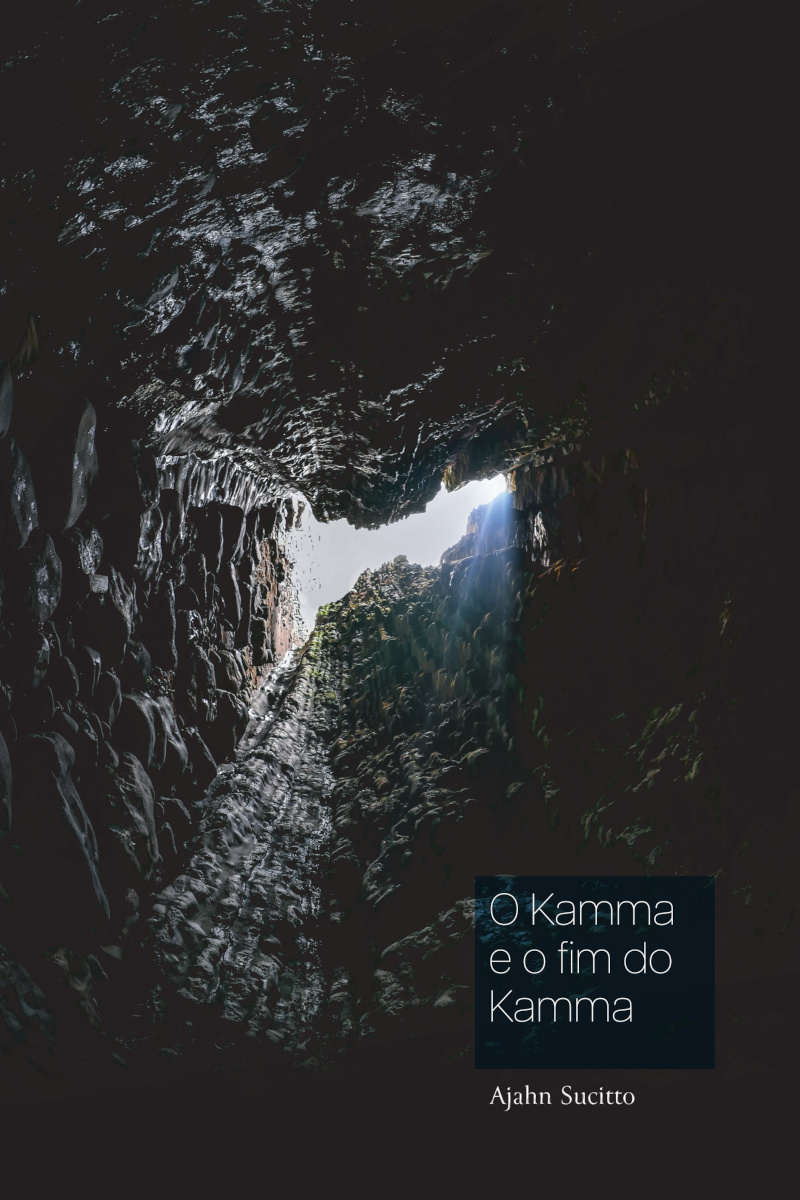
\includegraphics[height=\paperheight]{./desktop-cover.jpg}}
\fi

\cleartorecto
\thispagestyle{empty}
\vspace*{5em}

{\centering

\settowidth{\titleLength}{%
  {\Large\chapterTitleFont\textbf{\thetitle}}%
}

{\Large\chapterTitleFont\textbf{\thetitle}}\\[0.3\baselineskip]
\setlength{\xheight}{\heightof{X}}
\raisebox{0.5\xheight}{\color[gray]{0.4}\rule{\titleLength}{0.25pt}}\\[0.3\baselineskip]
{\itshape
\thesubtitle}

\vfill

\theauthor

\vspace*{5em}

}



\cleartoverso
\thispagestyle{empty}

{\copyrightsize
\centering
\setlength{\parindent}{0pt}%
\setlength{\parskip}{0.8\baselineskip}%

\thetitle\\
por \theauthor

Publicações Sumedhārāma\\
\href{https://sumedharama.pt}{www.sumedharama.pt}

Para distribuição gratuita\\
\textit{Sabbadānaṃ dhammadānaṃ jinati}\\
‘A oferta de Dhamma é superior a qualquer outra oferta.’

Este livro encontra-se disponível para distribuição gratuita em:\\
\href{https://sumedharama.pt}{www.sumedharama.pt}\\
\href{https://forestsangha.org}{www.forestsangha.org}

ISBN \theISBN

Copyright \copyright\ Publicações Sumedhārāma 2023

Tradutor: Alda Santos\\
Editor: Appamādo Bhikkhu\\
Capa: Phāsuko Bhikkhu\\
Formatação: Gambhīro Bhikkhu

Traduzido do original `Kamma and the End of Kamma'\\
Publicado por Amaravati Publications

Amaravati Buddhist Monastery\\
Hertfordshire, Great Britain\\
publications@amaravati.org

\vfill

{\footnotesize

Este trabalho está licenciado com uma Licença Creative Commons\\
Atribuição-NãoComercial-SemDerivações 4.0 Internacional.

Veja página \pageref{copyright-details} para mais detalhes sobre direitos e restrições desta licença.\\
Produzido com o sistema tipográfico \LaTeX. Fonte utilizada:\\
Gentium, Butler e Accanthis.

\theEditionInfo

}}


\cleartorecto
\thispagestyle{empty}

\mbox{}\vfill

\begin{verse}

{\itshape
Dedicado a

Goeren e Kyllie Lindeblad

e Patricia Buckle
}


\end{verse}

\vspace*{2\baselineskip}

\vfill\mbox{}


\clearpage

\begin{quote}

  ``O kamma deve ser conhecido. A causa através da qual o kamma entra em acção
  deve ser conhecida. A diversidade no kamma deve ser conhecida. O resultado do
  kamma deve ser conhecido. A cessação do kamma deve ser conhecida. O caminho da
  prática que leva à cessação do kamma deve ser conhecido. Assim foi dito. Por
  que razão foi dito?

  A intenção, digo"-vos, é kamma. Ao termos intenção, produzimos kamma através do
  corpo, da fala e da mente.

  E qual a causa através da qual o kamma entra em acção?

  O contacto, bhikkhus.

  E o que é a diversidade no kamma? Existe kamma a ser experienciado no inferno,
  kamma a ser experienciado no reino dos animais vulgares, kamma a ser
  experienciado no reino das sombras famintas, kamma a ser experienciado no
  mundo humano, kamma a ser experienciado nos mundos celestiais.

  E qual é o resultado do kamma? O resultado do kamma, digo"-vos, tem três tipos:
  aquele que surge aqui e agora, aquele que surge mais tarde (nesta vida) e
  aquele que surge depois disso\ldots{}

  E o que é a cessação do kamma? A partir da cessação do contacto dá"-se a
  cessação do kamma e apenas este nobre caminho óctuplo -- visão correcta,
  propósito correcto, discurso correcto, acção correcta, meio de subsistência
  correcto, esforço correcto, consciência correcta, concentração correcta --
  constitui o caminho da prática que conduz à cessação do kamma.

  Assim, quando um discípulo dos seres nobres compreende desta forma o kamma, a
  causa através da qual o kamma entra em acção, a diversidade no kamma, o
  resultado do kamma, a cessação do kamma e o caminho da prática que conduz à
  cessação do kamma, então compreende esta vida sagrada penetrante como a
  cessação do kamma.

  ``O kamma deve ser conhecido. A causa através da qual o kamma entra em acção
  \ldots{} A diversidade no kamma \ldots{} O resultado do kamma \ldots{} A
  cessação do kamma \ldots{} O caminho da prática que leva à cessação do kamma
  \ldots{}'' Assim foi dito e esta é a razão pela qual foi dito.''

  \href{https://suttacentral.net/an6.63/en/thanissaro}{AN 6.63}

\end{quote}


\cleartorecto
\tableofcontents*

\chapter{Prefácio}

Este livro foi desenvolvido a partir de uma série de palestras que dei no
decurso de alguns anos, principalmente no Mosteiro de Cittaviveka. Nestas
palestras explorei a relevância dos ensinamentos do Buddha sobre o kamma para a
prática da meditação. À primeira vista pode parecer que estes dois tópicos não
estão muito relacionados: o kamma é um ensinamento sobre o comportamento,
enquanto que a meditação, aparentemente, é sobre a ausência da acção, não é
verdade? Ou podemos ter a ideia de que: `O kamma é sobre aquilo que eu fui numa
vida anterior, aquilo ao qual eu estou preso agora e aquilo que será o meu
renascimento. O kamma é acerca de ser alguém, enquanto a meditação é acerca de
não ser seja quem for.' Não é assim. Espero que os textos que se seguem,
compilados a partir de palestras e que se tornaram ensaios, ajudem a clarificar
que os princípios do kamma ligam o comportamento `externo' à prática `interna'
da meditação. E que a meditação é um tipo de kamma -- o kamma que leva ao final
do kamma. Com efeito, `kamma e o fim do kamma' é um bom resumo daquilo que o
Buddha tinha para oferecer, como um caminho para o bem"-estar e para o Despertar.

\section{Os três conhecimentos do Buddha}

A experiência do Dhamma do Buddha tem a sua fundamentação nos `três
conhecimentos', constatações que se diz terem ocorrido sequencialmente ao
Buddha, numa noite. Apesar de praticar meditação e ascetismo a um nível muito
elevado, o Buddha sentiu que esta prática não lhe tinha dado frutos em termos da
sua busca da `transcendência da mortalidade'. Mas eis que, ao praticar mais
tranquilamente, surgiram três compreensões e, com estas, o seu objectivo foi
atingido.

A primeira destas compreensões foi a consciência de vidas anteriores. Este
conhecimento transcendeu a definição mais fundamental das nossas vidas -- a
divisão que ocorre na morte do corpo. Surgiu a compreensão de que aquilo que é
experienciado como uma `pessoa', constitui uma manifestação num processo em
decurso, ao invés de um eu único e isolado.

Entrar em contacto com esta força vital subjacente não constituiu um grande
conforto: expandiu a questão da existência para além da duração de uma única
vida, para um purgatório existencial constituído por um `vaguear' sem fim
(\emph{saṁsāra}). Contudo, por outro lado, existia uma consciência que tinha
transitado para essa panorâmica transpessoal. A porta para a `transcendência da
mortalidade' tinha começado a abrir"-se.

A segunda compreensão foi que a `direcção' desse vaguear não era aleatória --
este toma a sua direcção de acordo com a qualidade ética das acções que a pessoa
empreende. Surgiu o conhecimento que existem energias que são disruptivas ou
abusivas e que não sustentam a lucidez ou a saúde. Por outro lado, existem
energias que são harmoniosas, que alimentam ou que estão claramente em sintonia.
`Más' e `boas' (ou inadequadas / deletérias / `escuras' e
adequadas / salutares/ `luminosas' em termos Budistas) não são, consequentemente,
apenas juízos de valor impostos por uma sociedade, mas sim referências a
energias que são palpáveis em termos psicológicos, emocionais e físicos. A acção
empreendida de acordo com uma energia sã constitui um suporte para o bem"-estar e
para a harmonia, tal como o contrário tem o efeito oposto. Este constitui o
princípio de causa e efeito em termos éticos, ou `\emph{kamma"-vipāka}'.

Contudo, \emph{kamma"-vipāka} tem um significado mais profundo, que vai para além
de acções e resultados. Se a consciência cognitiva se apega a uma acção (física,
verbal ou psicológica) dá origem a uma consciência cognitiva à qual é dada uma
forma pessoal através desse mesmo apego. Esta acção cria a impressão de um eu,
que é o resultado dessa acção, e é `condimentada' pela qualidade ética dessa
acção. Dito de uma forma simples: não se trata tanto de eu criar kamma mas sim
do kamma `me' criar. Desta forma \emph{kamma"-vipāka} transcende a separação
entre acção e agente, mergulhando a consciência num campo de significado ético,
onde todas as acções formam e informam o `eu', o `meu', o `eu próprio'.

Da mesma forma, uma vez que o kamma surge numa maré de energia causal em
decurso, os resultados das acções podem ter lugar em vidas futuras. E isto
significa que o kamma nos prende ao processo de nascimento e morte -- algo que o
Buddha recordou em termos dramáticos:

\begin{quote}

  ``Há muito que (repetidamente) experienciaste a morte de uma mãe\ldots{} de um
  pai\ldots{} a morte de um irmão\ldots{} a morte de uma irmã\ldots{} a morte de
  um filho\ldots{} a morte de uma filha\ldots{} perda relativamente a
  familiares\ldots{} perda relativamente a riqueza\ldots{} perda relativamente a
  saúde\ldots{} As lágrimas que derramaste sobre a perda relativamente à doença
  enquanto transmigravas e vagueavas durante este longo, longo tempo -- a chorar
  e lamentar por estares associado ao que é desagradável, estares separado
  daquilo que é agradável -- têm um volume que supera o total da água dos quatro
  grandes oceanos.

  Porque é que isto sucede? A transmigração surge de um começo que não é
  passível de ser reconstituído. Não é evidente um ponto de começo, apesar dos
  seres dificultados pela ignorância e algemados pelo anseio continuarem a
  transmigrar e a vaguear. Assim, há muito, que experiencias tensão, dor, perda,
  há muito que preenches os cemitérios -- o suficiente para ficar desencantado
  com tudo o que é fabricado, o suficiente para ficar desapaixonado, o
  suficiente para ser libertado.''

  \href{https://suttacentral.net/sn15.3/en/thanissaro}{SN 15.3}

\end{quote}

Contudo, nesta admoestação existe igualmente a mensagem da possibilidade da
libertação deste \emph{saṁsāra}: através do acto de limpar e de largar, bem como
da `cessação' desses mesmos padrões de energia que transportam a causa e o
efeito -- e~o~`eu'.

Estes últimos foram vistos a partir do terceiro conhecimento, que trouxe a
libertação das `coisas fabricadas', das emoções, dos impulsos, das sensações e
das respostas que constituem a matéria"-prima do apego. Este conhecimento é a
compreensão dos preconceitos subjacentes (\emph{āsava}) que condicionam o apego
através do qual o \emph{saṁsāra} funciona.

\section{Renascimento e kamma}

O \emph{saṁsāra} não se expressa por intermédio de um corpo ou uma identidade.
Os corpos mantêm"-se dependentes das condições apenas durante uma vida. A
identidade -- por exemplo filha, mãe, director, inválido, etc. -- surge como
dependente de causas e condições. Aquilo que anteriormente foi referido como
`transmigração' não é `renascimento', mas o processo pelo qual uma corrente
duradoura de apego continua a gerar seres sencientes. Para além disso, esta
corrente não é algo que apenas ocorre na morte, mas que é alimentada de forma
contínua pelo kamma no momento presente. Através de uma tendência denominada
`devir', o \emph{kamma} forma algo semelhante a um código genético psicológico.
Este código, que constitui o padrão da herança cármica de cada indivíduo, é
formado através de processos dinâmicos chamados \emph{saṅkhāra}. Tal como o
código genético pessoal de cada um, o \emph{saṅkhāra} retém os esquissos
originais cármicos e, desta forma, permanecemos de dia para dia, em termos
relativos, a mesma pessoa.

Traduzido de forma variada como `formações', `formações volitivas',
`fabricações', etc., eu traduzo \emph{saṅkhāra} como `programas e padrões'.
Alguns destes programas são funções, tal como o metabolismo, que se encontram
ligados à força vital (\emph{ayusaṅkhāra}); alguns são veiculados pela
consciência que é gerada a partir de vidas anteriores; e alguns são formados
através de interacções da vida presente. Os programas mais significativos do
ponto de vista da transmigração são aqueles que enraízam o apego no nosso corpo
e na nossa mente. Estas são três `corrupções' -- a corrupção associada à
informação dos sentidos com sentimentos que vão desde o deleite à aversão; a
corrupção de `devir/tornar"-se algo' que gera a sensação de um eu autónomo; e a
corrupção da ignorância que obscurece a verdade acerca do \emph{saṁsāra}. Estas
corrupções são, na melhor das hipóteses, insatisfatórias e, na pior, causadoras
de tensão ou de dor, uma vez que programam de forma contínua a mente para
depender das características mutáveis da informação sensorial e para formar uma
identidade com base no terreno instável dos estados de espírito. Devido a este
desconforto existencial, a consciência não"-Desperta reage com hábitos de
ganância, aversão e confusão.

As boas notícias é que não estamos tão embutidos no \emph{saṁsāra} como parece.
Nem todos os aspectos da mente se encontram presos nas corrupções. Nós podemos
`ter consciência' das corrupções. E são apenas as corrupções que têm de ser
eliminadas. A acção que constitui uma preparação e que culmina com este corte é
o Nobre Caminho, o Caminho Óctuplo que o Buddha ensinou. Praticar este caminho é
o kamma que leva ao final do kamma.

Os ensinamentos sobre o kamma, sobre causa e efeito, proporcionam"-nos um Caminho
para a libertação. De forma abreviada, quando sabemos como funciona e temos as
capacidades e as ferramentas para desconstruir os programas da consciência
cognitiva, podemos parar de construir o \emph{saṁsāra}. Mais detalhadamente, os
ensinamentos do Buddha constituem um guia para a acção sustentada, tanto no
domínio externo como interno, em que a prática no domínio externo -- o de viver
uma vida moral e receptiva -- estabelece as directrizes e encoraja as
capacidades de forma a esclarecer o domínio interno. Factores causais
transpessoais, tais como o estar presente, a investigação, a concentração e a
equanimidade, podem proporcionar o efeito de abolição da modelação das
corrupções. Esta prática, mais do que extrair a pessoa do \emph{saṁsāra}, vai
desligar o processo do \emph{saṁsāra} para aquela consciência individual. O que
resta para aquele indivíduo pode ser resumido como um corpo e uma mente a
funcionarem durante esta vida, bem como uma consciência sem preconceitos, que
não participa na dinâmica da continuação dos renascimentos.

\section{O kamma por detrás deste livro}

Admito a existência de determinados enviesamentos. Existem muitas formas de
meditar e muitos professores experientes que podem constituir, neste campo, um
guia para os outros. Contudo, acontece com frequência que as pessoas necessitam
de ajuda na integração da atenção meditativa e da realização interior nas suas
vidas quotidianas. Isto, em parte, deve"-se ao facto da compreensão que as
pessoas ganham nos retiros de meditação não surgir do contexto da vida e das
actividades do dia a dia, mas sim de um ambiente especializado, tal como um
centro de meditação. Nestas condições, é dada uma atenção considerável a
temáticas como a consciência da respiração. Contudo, os temas que não são
relevantes, em termos imediatos, para a solidão e tranquilidade de estar sentado
num retiro, não recebem a atenção necessária para uma vida harmoniosa. As
relações interpessoais, quando saímos de um cenário de `ausência de contacto,
ausência de fala' de um retiro, parecem difíceis de integrar e, contudo, são
parte da vida de todos nós. De igual modo, se desenvolvemos a meditação no
sentido de aceitarmos pacificamente aquilo que está presente na nossa
consciência, como é que tomamos decisões no que diz respeito a escolhas
relativas à nossa subsistência e desenvolvemos planos sustentáveis para o
futuro? De igual forma, será que podemos obter orientação no tipo de
desenvolvimento pessoal que nos encoraja a sermos responsáveis, que nos permite
aceitar, partilhar ou questionar a autoridade, bem como tudo o resto de que a
sociedade necessita em termos de indivíduos com maturidade?

Infelizmente pode acontecer que as pessoas tenham experiências `espirituais'
válidas a um nível subtil mas permaneçam contudo bastante alheadas aos seus
próprios conceitos e ângulos mortos, em termos de acções e de interacções
pessoais. O que ajuda, na meditação e na vida do dia a dia, é aprender a manter
e a moderar o nosso propósito; como sermos sensíveis e autênticos para connosco
próprios e para com os outros; e como valorizarmos e ajustarmos a qualidade de
esforço que colocamos nas nossas vidas. Tudo isto, e mais, se insere sob o
tópico relativo ao kamma. Desta forma, temos necessidade de conhecer muito bem o
que constitui um kamma cuidadoso, em termos de contextos internos subtis e de
contextos externos mutáveis mais óbvios.

Assim, saliento a importância da compreensão da causalidade, como uma chave para
o Despertar, uma vez que transforma a prática num caminho a seguir na vida como
um todo, em vez de uma técnica de meditação. Isso enfatiza o facto de o
\emph{saṁsāra} ser um hábito e não um lugar. Desta forma, `sair do
\emph{saṁsāra}' não envolve indiferença para com o mundo, o corpo ou os outros,
nem se refere à conquista de uma área de território psico"-espiritual refinado.
Trata"-se do abandono dessa negatividade, dessa indiferença e dessa ânsia; e isso
significa cultivar e honrar o bom kamma. Por sua vez, esta constitui a base para
a total libertação do mal"-estar pessoal. A beleza e a profundidade da explanação
do Buddha é, para mim, esta unidade: Verdade, Virtude e Paz podem surgir a
partir do mesmo foco.

Estas palestras não foram dadas em série, mas sim espaçadas no tempo. Deste
modo, foi necessário trabalhá"-las em termos de revisão, de forma a homogeneizar
a linguagem, cortar as repetições e acrescentar material a que os ouvintes,
nessa mesma altura, tiveram acesso através de outras palestras. Mesmo depois de
tudo isto concretizado, pareceu"-me que alguns aspectos careciam de uma
explicação mais completa. Consequentemente, introduzi mais material escrito para
além do material apresentado nas palestras, de forma a ampliar este último.
Pensei igualmente em colocar algumas citações e notas do Cânone Pali e, como se
estava a tornar bastante teórico, intercalei os ensaios com algumas instruções
de meditação, breves mas relevantes. De qualquer modo, este livro não constitui
uma exposição passo-a-passo, mas sim um vislumbre de vários pontos de interesse
e uma revisão desses pontos a partir da perspetiva do kamma.

Gostaria de agradecer a ajuda de Ajahn Thaniya, que selecionou e comentou os
textos, e de Dorothea Bowen, que realizou o trabalho de revisão dos textos
centrais. Ocasionalmente, o manuscrito circulou também entre outros amigos
contemplativos, com vista a obter críticas e comentários: Ajahn Amaro, Ajahn
Kovida, Ajahn Viradhammo e os amigos de Ottawa, Irmã Cintāmani, David e Nimmala
Glendining, Gabriel Hodes, Douglas e Margaret Jones. Ajahn Kusalo ocupou"-se da
composição tipográfica e do \emph{design}. Este livro inclui ainda o bom
\emph{kamma} de muitas outras pessoas e faço votos que isto continue a guiá"-las
no sentido de um maior bem"-estar e liberdade.

\bigskip

{\raggedleft
Ajahn Sucitto\\
Cittaviveka, 2007
\par}


\chapter{Nota do Editor}

Ajahn Sucitto é conhecido e aclamado pela sua fabulosa e elaborada forma de
explanar o Dhamma, uma forma clara e objectiva, com uma precisão incisiva, mas
por vezes também poética. A sua escolha de palavras é exímia e cuidadosa, sendo
cada palavra apresentada fruto de uma estruturada e prolongada reflexão.

Queremos referir o trabalho árduo e dedicação que Alda Santos colocou nesta
tradução: colocar frases muito elaboradas e já por vezes longas no Inglês (e que
se transformam ainda mais longas no Português) de uma forma fluída e acessível é
uma mestria para a qual é necessário muito talento e engenho.

Este é um livro esclarecedor dos princípios e práticas do Dhamma e aconselhamos
o leitor a cultivar paciência e concentração na sua leitura, pois as palavras
escolhidas são por vezes as menos esperadas, de forma a `não passarmos por cima'
e a nos determos no significado mais profundo daquilo que está a ser
transmitido. Frases por vezes longas requerem uma leitura cuidadosa, sendo até
por vezes necessário repetir a leitura para que se possa absorver o significado
em toda a sua profundidade e plenitude. Mas vale a pena, pois a riqueza e
aprimoramento deste texto pode deixar uma marca indelével no praticante, com
resultados inequívocos para a sua investigação, que poderão vir a constituir um
farol na sua prática e investigação, para o resto da sua vida.

As sugestões de meditação apresentadas constituem também um forte método de
realização interior a ser colocado em prática.

Deixamos assim aqui esta nota de agradecimento e encorajamento.

Que seja cumprido o propósito do Dhamma.


% Page 1 is the first page of the first chapter.
\mainmatter

\chapterNote{Uma panorâmica sobre os ensinamentos do Buddha acerca do kamma}

\chapter{Onde Existe uma Vontade Existe um Caminho}

\tocChapterNote{Uma panorâmica sobre os ensinamentos do Buddha acerca do kamma}

\begin{quote}
  ``E, bhikkhus, como é que uma pessoa vive simultaneamente para o seu próprio
  bem e para o dos outros? Ela própria pratica no sentido da remoção da cobiça,
  do ódio e da ilusão e encoraja igualmente os outros a fazerem o mesmo.''

  \quoteRef{\href{https://suttacentral.net/an4.96/en/thanissaro}{AN 4.96}}
\end{quote}

O que é o `kamma' e qual a sua relação com o Despertar? Ora bem, tomado como uma
palavra, `kamma' é a versão em língua Pali do termo em sânscrito `karma', que
tem vindo a ser usado no inglês coloquial\footnote{E também no português
  coloquial (N.T.).} com um significado semelhante a `destino'. Neste sentido,
esta noção pode apoiar uma aceitação passiva das circunstâncias: se algo corre
mal podemos sempre dizer que `era o meu carma', querendo dizer que tinha de
acontecer. Onde a ideia de base realmente se perde é quando é usada para pactuar
com determinadas acções, como por exemplo `ser ladrão é o meu carma'. Se este
fosse o significado do carma tirar"-nos-ia a responsabilidade sobre as nossas
vidas. Para além disso, não haveria qualquer forma de nos orientarmos de modo a
sairmos das nossas circunstâncias ou da nossa história passada -- que é aquilo
em que consiste o Despertar. Contudo, `kamma', no sentido em que o Buddha
ensinou, significa acção adequada ou inadequada -- algo que fazemos agora. É o
aspecto activo de um processo de causa e efeito conhecido como
\emph{kamma"-vipāka}, no qual \emph{vipāka} ou `kamma antigo' significa o efeito,
o resultado de acções anteriores. E, em larga medida, vemo"-nos envolvidos nos
resultados das nossas acções.

Não obstante, enquanto `acção', o kamma apoia a escolha. Podemos escolher as
acções que vamos empreender. Causa e efeito regulam a actividade dos vulcões,
das plantas e dos sistemas planetários, mas o kamma diz respeito especificamente
aos seres que têm poder de escolha sobre aquilo que causam -- ou seja, o leitor
e eu. Da mesma forma, nem tudo o que experienciamos é devido ao kamma antigo
(para além do que diz respeito a termos nascido).\pagenote{Onde existe uma
  vontade existe um caminho:

  O Buddha sublinhou que tudo aquilo que experienciamos não se encontra
  necessariamente relacionado especificamente com as nossas acções anteriores:

  ``\ldots algumas sensações surgem a partir de mucos\ldots{} a partir de ventos
  internos\ldots{} a partir de desequilíbrios dos humores do corpo\ldots{} da
  mudança das estações\ldots{} do cuidado irregular do corpo\ldots{} de
  agressões\ldots{} do resultado do kamma. Que algumas sensações surgem em
  resultado do kamma, podemos saber por nós próprios e todos compreendemos que
  isso acontece. Agora, quaisquer contemporâneos ou sábios que defendem a
  doutrina ou ponto de vista que seja o que for que o indivíduo experiencie --
  prazer, dor, nem prazer nem dor -- é inteiramente causado por aquilo que foi
  feito anteriormente -- ultrapassam aquilo que eles próprios sabem e aquilo em
  que as pessoas em geral concordam. Desta forma afirmo que esses contemporâneos
  ou sábios estão errados.''

  \href{https://suttacentral.net/sn36.21/en/bodhi}{SN 36.21}, ver também
  \href{https://suttacentral.net/mn136/en/thanissaro}{MN 136}.}
Assim, se adoecemos ou se formos apanhados num terramoto, não é necessariamente
porque tenhamos praticado más acções numa vida anterior. Em vez disso, o kamma
centra"-se na nossa intenção ou `volição'
(\emph{cetanā})\pagenote{Intenção/volição é kamma: por exemplo
  \href{https://suttacentral.net/an6.63/en/thanissaro}{AN 6.63}. É importante
  reconhecer que `intenção' neste contexto não requer necessariamente
  deliberação. \emph{Cetanā} refere"-se à `inclinação' ou à `intenção' do
  coração, que se encontra subjacente ao pensamento e alimenta a emoção.}
actual. Desta forma, os ensinamentos sobre o kamma encorajam um sentido de
responsabilidade relativa à acção -- a responsabilidade de prestar atenção às
muitas escolhas conscientes e semiconscientes que realizamos, em relação ao que
fazemos. Isto significa que, neste preciso momento, temos possibilidade de
escolha sobre a forma como o futuro vai decorrer: se nos vamos sentir contentes
e tranquilos connosco próprios, ou ansiosos e deprimidos, dependerá das nossas
acções neste momento. E, de igual forma, através das nossas acções neste
momento, podemos ser libertados do passado, do presente e do futuro. É isso que
resulta do Despertar para o kamma.

\subsection{Kamma físico, verbal e mental}

`Kamma' significa `acção', num sentido que vai para além do físico. Inclui
também a acção verbal -- quer insultemos e gritemos com as pessoas ou digamos
coisas verdadeiras e fiáveis. E isso inclui o `discurso interno' do pensamento!
Mas, na realidade, o kamma das nossas respostas emocionais -- o kamma `mental'
(ou `do coração') -- é o mais forte.\pagenote{O kamma mental é o mais forte.
  Este é o tema de um debate, registado em M.56, no qual o Buddha explica de
  forma convincente:

  ``Destes três tipos de acção\ldots{} descrevo a acção
  mental como a mais repreensível para a realização de acção malévola, e não
  tanto a acção física ou verbal.''} As respostas -- e as propensões sobre as
quais elas se baseiam -- regem as acções do corpo e do discurso, originando
igualmente resultados no domínio das emoções, das atitudes e dos estados de
espírito. De igual modo, as nossas acções físicas ou verbais resultam apenas de
convicções, pressupostos, interpretações e atitudes (ou seja, todos provenientes
da mente). Por si próprio, o corpo não faz bem nem mal -- estas qualidades
éticas encontram"-se enraizadas na mente que inicia o acto físico. Passa"-se o
mesmo com a fala e o pensamento: a linguagem é neutra -- é a bondade ou a
malícia da mente, que utiliza a linguagem e os conceitos, que produz resultados
felizes ou infelizes.

Considerarmos o kamma sob este prisma motiva"-nos a libertar a mente da má
vontade ou da cobiça, porque estas conduzem a acções verbais ou físicas que
deixam uma marca desagradável: geram rudez, apego e obstinação e, mais tarde,
preocupação, arrependimento e dúvida. Por outro lado, acções e pensamentos
baseados na compaixão proporcionam à mente clareza e afecto. Daí os ensinamentos
sobre causa e efeito: eles são um lembrete para verificarmos, investigarmos e
purificarmos os estados de espírito associados à acção, seja ela qual for. Tal
como as nossas acções trazem conflito ou harmonia ao contexto em que vivemos,
controlar o kamma permite"-nos ter um efeito positivo no mundo que nos rodeia.
Perceber o kamma desta forma também possibilita que percebamos amplamente que o
nosso bem"-estar não é independente do modo como agimos para com os outros.

\subsection{As dinâmicas do kamma}

A lei do kamma define que um efeito ou resultado é inevitável a partir de uma
causa activa. Se eu ofendo e maltrato alguém hoje, isto tem como efeito que essa
pessoa se sente magoada e isso quer dizer que ela, provavelmente, irá ser
desagradável comigo no futuro. É igualmente provável que essa acção tenha
efeitos imediatos sobre a minha própria mente: agitação e remorso. Ou pode
acontecer que me habitue a agir dessa forma: de modo que continuo a agir de
forma ofensiva, desenvolvo uma mentalidade insensível e perco amigos. Desta
forma os efeitos acumulam"-se, tanto em termos de estados de espírito (ofensas e
remorsos), como também de estruturas comportamentais (um padrão ou uma
programação de ser egocêntrico ou de possuir uma língua afiada). O que é
verdadeiramente problemático são os `programas', as `formações' (ou, em
linguagem budista, \emph{saṅkhāra}) em decurso. Estes padrões de comportamento
tornam"-se parte da nossa identidade e, uma vez que não conseguimos ver para além
dos nossos próprios hábitos entranhados, estes padrões e programas sustêm o
girar, o \emph{saṁsāra}, de causa e efeito.

Desta forma, se nos queremos libertar, é importante, controlar o modo como
estamos a funcionar. E isso é possível porque o processo \emph{kamma"-vipāka}
forma circuitos de \emph{feedback} de sensações mentais de tensão ou de
agitação, ou de tranquilidade, que podemos contemplar e ter em consideração.
Para além disso, podemos responder de diferentes maneiras ao resultado das
nossas acções - de forma a que cada efeito não venha a inevitavelmente gerar uma
causa correspondente. Eis a escolha: posso fazer uma pausa, sair do estado de
espírito de irritação ou de imprudência, prestar"-lhe a devida atenção e tentar
fazer melhor no futuro. Este é o primeiro passo no sentido da libertação.

Os ensinamentos do kamma são mais facilmente acessíveis no contexto do
comportamento exterior. O Buddha viu que a clareza relativamente ao
comportamento proporciona uma via pragmática, através da qual o sofrimento e a
tensão podem ser evitados, e a paz, a confiança e a clareza podem ser geradas.
Assim, o Buddha falou de kamma escuro -- acções tais como assassínio, roubo,
falsidade e abuso sexual, que conduzem a maus resultados -- e kamma luminoso --
acções tais como bondade, generosidade e honestidade, que fazem o inverso. O
Buddha falou igualmente de uma mistura de kamma escuro e luminoso -- acções que
possuem algumas boas intenções mas que são conduzidas de forma inadequada. Um
exemplo disto seria termos o objetivo de proteger e cuidar da nossa família, mas
fazê"-lo de um modo prejudicial para os nossos vizinhos.

O kamma é também dinâmico: agimos de acordo com informação que recebemos e, à
medida que recebemos de volta os resultados agradáveis ou desagradáveis, as
nossas acções subsequentes vão sendo moldadas. Contudo, uma vez que parte deste
retorno não ocorre imediatamente e pode mesmo levar anos a suceder, existem
aspectos deste circuito de retorno que são caóticos. Isto significa que o nosso
ritmo de aprendizagem não acompanha necessariamente o ritmo ao qual podemos
desenvolver novas acções. Estivemos a poluir alegremente a atmosfera durante
décadas, até se tornar claro o que se estava a passar e, por essa altura, outras
acções já tinham sido realizadas -- estabeleceram"-se indústrias e estilos de
vida dependentes de recursos não sustentáveis, o que torna a mudança mais
complicada.

Este ponto é significativo: encoraja"-nos a esforçarmo"-nos por clarificar a
consciência da mente e dos seus impulsos. É necessário que investiguemos as
nossas mentes e os programas mentais frequentemente e de forma mais detalhada.
Então aí é possível interromper o circuito de retorno com informação que pára ou
que modera os nossos impulsos. Esta informação é o kamma que leva ao final do
kamma e constitui o eixo dos ensinamentos do Buddha.\pagenote{Escuro, luminoso,
  ambos e o kamma que conduz ao fim do kamma:

  ``E qual é o kamma que não é nem escuro nem luminoso, que não tem resultados
  nem escuros nem luminosos, e que conduz ao fim do kamma? A intenção para
  abandonar aí mesmo este kamma que é escuro e com resultados escuros\ldots{}
  luminoso e com resultados luminosos\ldots{} escuro e luminoso e com resultados
  escuros e luminosos.''

  \href{https://suttacentral.net/an4.232/en/sujato}{AN 4.232}, ver também
  \href{https://suttacentral.net/mn57/en/bodhi}{MN 57.7-11}.}
Ao ser plenamente realizado, pode levar não apenas a mudanças no
comportamento, mas à libertação completa.

\subsection{Nascimento: a herança da causa e efeito}

A libertação completa significa sair por completo do processo de causa e efeito.
Este processo é aquilo que estamos a experienciar neste momento. Nascer é kamma
antigo e trouxe"-nos ao imbróglio da existência no domínio da causa e efeito, com
o potencial de continuar a girar nele. Tendo herdado o efeito de sermos
corpóreos, somos afectados por comida, saúde e clima. E, juntamente com isto,
vem o potencial para defender, procurar comida e procriar. A mente está
sintonizada para responder a tudo isto de forma instintiva, com impulsos de
luta, paralisação ou fuga, que podem surgir num abrir e fechar de olhos. E com a
mente vem a consciência do envelhecimento, da doença e da morte. E, com isso, a
separação daqueles que amamos, com o efeito desagradável que isso tem em nós; e
ainda, o facto de sermos aparentemente impotentes para fazer seja o que for
acerca de tudo isto. Assim, o girar do \emph{saṁsāra} prende"-nos no seu
movimento giratório.

O kamma antigo traduz"-se igualmente em todos os programas sociais e
comportamentais que nos dizem como devemos funcionar em termos de costumes e
atitudes. Psicologicamente, experienciamos a necessidade de pertença, de
compreensão e de nos sentirmos em paz com as circunstâncias nas quais estamos
inseridos. Esta constitui a base para o kamma novo: uma das nossas acções
mentais mais contínuas é a de interpretação e de arquivo de experiências, de
forma a extrairmos significados e propósitos. De igual modo, apanhamos muita
informação das outras pessoas, incluindo preconceitos e informação redundante,
assim como bons conselhos. Este kamma mental forma o programa, o modo de pensar,
através do qual interpretamos a nossa experiência presente. Instalado e
modificado ocasionalmente, este programa aplica, em qualquer momento, uma
interpretação da experiência presente para nos dizer `como algo é'. E isto vai
muito além da definição objectiva: `Será seguro, será amigável, será permitido,
serei valorizado ao adquirir isto' e por aí adiante -- torna"-se um filtro de
impressões que nos ajuda a tomar muitas decisões instantâneas nas nossas vidas.
Contudo, qual a fiabilidade deste processo crucial?

Surgem memórias que nos levam a ter determinada inclinação, surgem condições
físicas que afectam a nossa disposição, a duração da atenção varia e o resultado
de uma conversa que tivemos há uma hora atrás ainda está a agitar os nossos
corações. Entretanto o nosso contexto social liga"-nos aos efeitos das mentes das
outras pessoas, cada uma com as suas próprias interpretações e os seus
mal"-entendidos, de forma que também somos afectados por isso. Os programas são
transferidos, ou desencadeiam outros programas, e as nossas mentes são apanhadas
num turbilhão de impressões, sendo que qualquer delas pode a qualquer momento
despoletar certos impulsos.

Então, a parte verdadeiramente crucial daquilo que herdamos é a `mente' -- uma
consciência afectiva"-receptiva complexa que transporta um elevado potencial para
mais kamma. Através da mente podemos estar conscientes de algo, reflectir e
desenvolvermo"-nos de acordo com os resultados daquilo que fazemos e dizemos.
Podemos aprender. E, à medida que as nossas respostas ampliam e intensificam a
nossa experiência, podemos ser criativos. Podemos concentrar"-nos numa ideia e
desenvolvê"-la numa invenção fantástica ou numa belíssima obra de arte. Contudo,
por outro lado, podemos ser assoberbados por uma emoção desenfreada. Se a
disposição é de desconfiança ou de ressentimento, podemos elaborar pontos de
vista maléficos sobre o mundo e cometer atrocidades. Há uma grande amplitude de
possibilidades: o Buddha refere muitos domínios infelizes e infernais que
resultam de acções imorais ou `kamma escuro'. As boas notícias é que os domínios
felizes e celestiais, onde podemos nascer em resultado de kamma bom ou
`luminoso', são ainda mais numerosos.\pagenote{Tanto
  \href{https://suttacentral.net/mn135/en/bodhi}{MN 135} como
  \href{https://suttacentral.net/mn136/en/thanissaro}{MN 136} apontam para
  diversos destinos localizados em reinos celestiais ou infernais como o
  resultado de actos realizados nesta vida.}
Seja como for não se acaba tudo
numa vida! Hoje em dia as pessoas gostam de interpretar estes `domínios'
cosmológicos como estados psicológicos -- mas mesmo sob este ponto de vista, o
kamma, luminoso ou escuro, é acção que vai dar origem a um estado de existência
futuro. E, à primeira vista, parece que não existe saída possível:
experienciamos as nossas vidas como estando inseridas num contínuo dinâmico que
nos afecta e nos modela -- tal como nós o afectamos e modelamos.

Pensando bem, o processo de \emph{kamma"-vipāka} é como o de um oceano que nos
pode elevar, engolir ou transportar em qualquer direcção. Funciona através de
uma interação contínua entre os efeitos herdados, à medida que eles surgem no
presente, e a gama de respostas consequentes e tendências para agir. O passado
não está morto: os seus efeitos transportam potencial. E o futuro surgirá de
acordo com a forma como agimos com base nisso.

\subsection{Despertar para a causa e efeito}

À primeira vista, esta perspetiva do kamma parece ser, não de libertação, mas
sim de aprisionamento. Mas quando se está na cela de uma prisão, começa"-se a
investigá"-la mais detalhadamente para ver, primeiro, como é que se pode torná"-la
mais habitável e, depois, como sair dela.

Em primeiro lugar, se temos de gerar kamma, podemos, pelo menos, determinar se
este vai ser luminoso ou escuro. Lembre"-se que existe a possibilidade de
escolha: o kamma depende da volição mental, ou da intenção, quer se trate de uma
intenção cuidadosamente ponderada, de uma necessidade compulsiva ou de um
reflexo psicológico. Neste sentido, `intenção' não é apenas um plano deliberado.
Com efeito, lá bem no âmago do nosso enigma encontra"-se o facto de nem sempre
estarmos assim tão claros relativamente ao que fazemos e às razões subjacentes.
Podemos estar a funcionar em modo automático, ou com uma atenção turva ou
desfasada, mas ainda assim a agir ou a sermos movidos pelo `empurrão' de uma
paixão ou hábito. Para muitos de nós, o problema principal não é a intenção
deliberadamente malévola, mas sim a acção baseada quer em confusão, desatenção
ou num mal"-entendido. Muitos dos nossos problemas têm origem no facto de
estarmos `pre"-ocupados' ou emperrados em hábitos. Dessa forma, não trazemos uma
atenção clara às nossas acções. Ou pensamos que as coisas estão bem e, portanto,
não precisamos de nos preocupar; ou que não estão bem, mas que não temos
qualquer poder de decisão sobre o assunto. Mas pelo menos existe sempre a
escolha de investigar o kamma, e é aí que começa a reviravolta.

Isto sucede porque a volição mental pode ser compreendida e bem dirigida, se
estivermos cientes dela com atenção e sabedoria. Podemos olhar para os nossos
pensamentos e impulsos, fazer uma pausa e recebê"-los de uma forma mais plena e,
deste modo, sentir o tom luminoso ou escuro que trazem à mente. Isto ajuda"-nos a
perceber como e quando devemos agir. Por exemplo, o sentimento resultante de
kamma luminoso encoraja alguém que tenha tido o bom fortúnio de herdar riqueza
ou inteligência, a partilhá"-la. Assim, essa pessoa irá fazer a melhor utilização
desse kamma antigo ao torná"-lo kamma novo brilhante. Com efeito, quando alguém
não partilha o seu bom fortúnio, o efeito agradável a ele associado estraga"-se:
as pessoas ricas que são egoístas e complacentes, em geral, querem sempre mais
ou tornam"-se avarentas e obcecadas consigo próprias.

Por outro lado, podemos estar a experienciar o efeito nefasto de sermos
agredidos ou magoados, ou de estarmos ansiosos, mas decidirmos não cobrar isso a
outra pessoa. Ou também podemos começar a investigar e a acalmar essa
disposição, e até a compreender o que causou esses efeitos. Neste tipo de acção,
a volição não progride para um estado futuro, mas desenvolve"-se no sentido de
compreendermos o estado presente. Esta compreensão não é uma questão de
percebermos todos os porquês e motivos do kamma: na realidade os detalhes das
razões pelas quais experienciamos uma determinada disposição, intuição ou
impulso num determinado momento são demasiado complexos para serem
compreendidos, é como tentar compreender que rio ou nuvem deu origem a qual gota
de água no oceano.\pagenote{De acordo com
  \href{https://suttacentral.net/an4.77/en/thanissaro}{AN 4.77}, o funcionamento
  preciso do kamma é um dos quatro `imponderáveis'. Ponderar sobre estes leva à
  `loucura ou enfado'. Os restantes são: a dimensão do poder de um Buddha, a
  dimensão dos poderes de alguém em estado de absorção (\emph{jhāna}) e a origem
  do mundo.}
O aspecto mais importante relativamente a compreendermos o kamma é
entrarmos nas correntes subjacentes da mente e alterarmos a maré dos efeitos. E
para fazermos isso é necessário que cultivemos uma consciência firme, clara e
não agitada por estados de humor e sensações. Este reconhecimento, baseado na
`visão correcta', traz o `propósito correcto', a activação do Caminho Óctuplo
que nos liberta do sofrimento e do stress.\pagenote{A Visão Correta é
  considerada como fundamental em numerosos \emph{suttas}, sendo descrita da
  seguinte forma:

  ``Existe aquilo que é dado, aquilo que é oferecido e aquilo que é sacrificado;
  existe o fruto e o resultado de boas e más ações; existe este mundo e o outro
  mundo; existe mãe e pai; existem seres que renascem espontaneamente; existem
  neste mundo contemplativos bons e virtuosos, e sábios que realizaram por si
  próprios através de conhecimento directo e declaram este mundo e o outro
  mundo.'' \href{https://suttacentral.net/mn117/en/bodhi}{MN 117.5}

  ``O Propósito Correto é um propósito que é desprovido, ou se afasta, de causar
  dano, da crueldade e do desejo sensual.''
  \href{https://suttacentral.net/mn19/en/bodhi}{MN 19}}

Um aspecto que se torna evidente em relação à corrente da mente é que seja em
que sentido for que ela esteja a fluir, temos a tendência a ficar presos nela.
Queremos proteger e manter um estado feliz e sentimo"-nos mal relativamente ao
seu eventual declínio ou desaparecimento -- a nossa identidade fica baseada
nesse estado. Por outro lado, sentimo"-nos encalhados e desesperados
relativamente aos estados de infelicidade. Desta forma, todo o kamma origina,
define e nos enquadra em termos psicológicos. Portanto, até o bom kamma confere
uma certa desvantagem, pois ainda implica um investimento na área do kamma.
Nessa área, a roda da sorte pode girar no sentido descendente: podemos ser
atacados e certamente adoeceremos, sentiremos dor e enfrentaremos separações.
Podemos igualmente ser arrebatados por alguma paixão ou impulso avassalador e
fazermos algo do qual nos arrependamos para o resto da vida. Assim, o Buddha
apontou para uma melhor opção: sair desta arena do kamma, aprofundando a
consciência para além do alcance do kamma e do \emph{vipāka}. Este é o objetivo
que leva ao Despertar e à total libertação.

\subsection{Kamma e o `eu\kern -0.5pt'}

No seu verdadeiro sentido, a libertação do kamma é a libertação da mente do
ciclo de causa e efeito. É um processo de nos distanciarmos mental e
emocionalmente de qualquer estado e de o ver apenas como um estado, sem reacções
e atitudes. Esta capacidade simples, que muitos de nós conseguimos ter
ocasionalmente, é aquilo que desenvolvemos na prática budista. De uma forma mais
radical, significa distanciarmo"-nos do programa que afirma que `a minha vida
encontra"-se preenchida se eu tiver ou estiver num determinado estado\ldots{}
neste ou noutro mundo'. Esta é a perspetiva que perpetua o kamma. Quando esta
perspetiva constitui a lente através da qual vemos, iremos continuar a procurar,
ou a imaginar, um determinado estado subjetivo imutável no qual nos encontramos,
podemos vir a estar, ou que poderemos possuir. Já alguém, alguma vez, encontrou
algum estado com estas características? Esta `perspetiva de si próprio'
agarra"-se aos corpos, aos sentimentos, às noções, aos programas mentais e à
informação sensorial sob a forma `isto sou eu, isto é meu, isto sou eu próprio'.
Mas já encontraram algum estado no qual podem ficar para sempre e que nunca vos
desilude?

E quem é este `eu' que pode possuir alguma coisa e o que é que ele ou ela poderá
ser? Como é que `eu' posso ter posse das emoções, se as agradáveis se vão embora
quando `eu' não quero, e as desagradáveis instalam"-se sem serem convidadas? Como
é que `eu' posso ser os meus impulsos, as minhas ideias ou as minhas disposições
se, quando estes surgem, condicionam"-se entre eles e desaparecem como se de
cúmplices se tratassem? Não podemos dizer que os sentimentos constituem um `eu'
permanente, uma vez que eles vão e vêm, e alteram"-se. Nem sequer podemos chamar
isso de propensão para sentir `um eu', uma vez que também isso se encontra
dependente de estarmos acordados ou adormecidos, atordoados, desatentos ou
hipersensíveis. Para além disso, os significados pessoais que projectamos na
vida e as reacções e as respostas psicológicas que são as nossas impressões
digitais, estão também sujeitas a alterações. A dinâmica deste processo é tão
contínua, que dá origem a uma sensação de solidez, mas não se consegue encontrar
uma essência ou uma entidade central permanente.

Se aprofundarmos este tópico, algo que seja `eu' teria de ser independente --
apenas `eu' e não parte de outra coisa. Mas a existência e constituição do
corpo, por exemplo, encontra"-se dependente dos pais e da comida, bem como de
muitos outros factores. Não surge de forma independente. Quando cortamos o
cabelo ou as unhas, não perdemos o sentido de `eu', de forma que o `eu' não pode
estar associado à corporalidade. E os sentimentos e a propensão para sentir não
estão dependentes de `algo' mais? Vemos algo, sentimos algo -- que tipo de ver e
de sentir poderia acontecer sem um objecto? Para além disso, o `eu' não pode
estar associado a estados e actividades mentais -- estes não surgem dependentes
de estados físicos ou de outros estados ou outras actividades mentais? Então,
mais uma vez, se corpo, sentimentos e informação sensorial fossem o meu `eu',
certamente que eu poderia decidir `que sejam desta forma e não de outra'. Mas,
efetivamente, eles seguem o seu próprio caminho, o caminho da `causa e efeito'.
Então o que é o `eu'? E o que é que se passa aqui?

Podemos não conseguir encontrar algo ao qual chamar `eu', contudo experienciamos
`ser algo' de forma contínua; temos um sentimento contínuo de `eu sou'. Como é
que isto acontece? Devido à consciência -- cuja função normal é discriminar a
experiência, em termos de um sujeito e um objecto separados. Mas sujeito e
objecto constituem inferências e não realidades, e eles estão dependentes um do
outro -- não podemos ter a sensação de um sujeito sem um objecto e vice"-versa.
Agora, quando a consciência mental se dirige para a nossa dimensão interna,
subjectiva, mais uma vez separa sujeito de objecto, com uma inferência de `eu',
como o propagador, e de `mim próprio', como aquele que herda os estados de
espírito, as disposições, os pensamentos e tudo o resto. (Tal como em `aqui
estou eu a sentir"-me confundido comigo próprio, porque esta atitude não parece
minha -- estou"-me a sentir fora de mim neste momento'.)

Cada sensação, cada pensamento, cada sentimento que ocorre é classificado como
`aquilo que sou -- isto é meu' (apesar de mudarem e desaparecerem); ou então
mantemos a noção que `eu não sou assim' (apesar de `eu' ser definido em termos
de informação que recebo e que me afecta). Qualquer uma destas duas actividades
psicológicas instintivas de `eu ser' (`eu sou isto' ou `eu sou algo que não
isto') determina continuamente um sentido de eu próprio, de formas que geram
ainda mais uma autodefinição específica. Contudo, uma vez que `eu' não consigo
agarrar"-me àquilo que quero e não consigo escapar daquilo que não quero, a
disposição subjacente do `eu' fica inquieta e insatisfeita. Persisto em
encontrar o estado bom\ldots{}, mas ainda não é bem este. Assim, existe mal"-estar.
A libertação deste mal"-estar e desta tensão é, assim, sinónimo da nossa
Libertação do `eu' insatisfeito.

\subsection{Desenvolver"-se a si próprio para se libertar do `eu\kern -0.5pt'}

A forte tendência para manter um `eu' -- denominado `tornar"-se/devir' ou `ser'
(\emph{bhava}), encapsula o sentido do `eu' e de `mim' como uma noção, uma
impressão de si próprio que perdura como um ponto de referência para a minha
mente, independentemente daquilo em que ela tenha estado envolvida. Desta forma,
este `eu' não é uma entidade mas sim um padrão, um `programa de construção de si
próprio' (\emph{ahaṁkāra}), constituído por comportamentos emocionais e
psicológicos. Estes dão origem à sensação de que: `esta é a forma como funciono,
estas são as minhas opiniões, esta é a minha história' e, consequentemente,
existe a impressão de ser um `eu' neste e naquele estado, com estratégias no
sentido de continuar dessa forma, de a incrementar ou de sair dela. Mas tudo
isto não constitui uma identidade, algo fixo, sendo sim um processo de `ser isto
e tornar"-se aquilo'. `Tornar"-se' (ou `devir') é o programa central por detrás do
kamma. É a razão pela qual existe tanta actividade mental. Mas devido a ser uma
actividade, não pode parar. Contudo, este `devir' está enraizado e é instintivo:
não pára através do raciocínio. Como instinto que é, tem de ser travado no âmago
do coração, sendo este um processo que envolve conduzir o impulso da intenção a
clarificar o ponto de vista que cria o `eu'.

Primeiro temos de criar força, perícia, capacidade. Assim, muitos dos
ensinamentos do Buddha favorecem o `devir' em termos de nos tornarmos mais
claros, mais estáveis, mais afáveis.\pagenote{Ou seja, aquele que se desenvolve
  faz com que estados positivos, tais como a calma e a bondade, se concretizem.
  Alguém assim tem: ``realização em termos de virtude; de desejo; de si próprio;
  de diligência; de atenção cuidadosa.''
  \href{https://suttacentral.net/sn45.71-75/en/bodhi}{SN 45.71}}
Geramos bom kamma através de actos de generosidade, bondade e através do abandono dos
comportamentos que causam dano. Tornamo"-nos pessoas mais calmas, mais
inteligentes. A visão correcta encoraja consciência dos resultados daquilo que
fazemos, consciência de partilharmos este mundo com outros e consciência da
importância do nosso domínio interior, psicológico, sobre o domínio do contacto
dos sentidos. Se o sentido mais profundo de realização, através da compaixão e
da calma, se estabelece, podemos então largar o `conseguir, ganhar e agarrar' --
principais causas de tensão. Podemos divergir da necessidade de eficiência a
curto prazo, de conveniência, de sucesso, de conforto e de atracção sexual.
Estaremos, então, no caminho certo para a libertação.

Consideremos o cenário social: no ocidente, muitos de nós podemos viver com
conforto físico, contudo, por estamos constantemente a ser confrontados com
comodidades mais refinadas ou com alterações constantes nos padrões de
comparação, não existe um grande contentamento. E existem também pressões
sociais e de grupo. Uma pessoa pode muito bem sentir que o seu emprego está em
risco se a roupa que está a usar não for a `correcta', de forma que tem de ter
este aspecto em consideração. As pessoas podem tornar"-se deprimidas, mesmo
neuróticas, se os seus corpos não estiverem à altura dos padrões actuais de
beleza, ou se as suas personalidades não forem suficientemente vivas, cínicas ou
sórdidas (dependendo da moda). Queremos evitar perder boas oportunidades e
receamos a solidão de não ter amigos. Por isso pode existir um sentimento de
nervosismo ou de insegurança relativos a falta de adequação, que nos privam de
um sentimento de confiança no nosso valor inato enquanto seres humanos.

Então, somente por causa disto, é importante que sintamos e nos definamos como
`estando' afastados destas correntes, mais que não seja para chegarmos a uma
base mais firme. E o que realmente nos ajuda é acalmar e apaziguar a mente, e
desenvolvermo"-nos naquilo que confere maiores benefícios, vivendo a nossa vida
com autenticidade. Podemos cultivar uma simplicidade de necessidades e um
sentido de sinceridade e de integridade. Podemos ter contentamento através do
reconhecimento do bem em nós próprios e nos outros. As pessoas têm problemas e
defeitos, mas é sábio honrar a bondade que todos temos. É igualmente sensato
encarar com compaixão as nossas tendências no sentido da reactividade e da
confusão, isto porque a forma como dispomos a nossa atenção cria o âmbito no
qual a mente habita. De modo que, se pudermos começar por experienciar clareza e
empatia relativamente a nós próprios e aos outros, damos por nós a viver de uma
forma mais grata e equilibrada, encorajando o desenvolvimento da bondade. Assim,
podemos dirigirmo"-nos para o bom kamma, desenvolvendo uma base que constitui um
real apoio para o nosso bem"-estar.

Trabalhar desta forma com as impressões da mente pode trazer mudanças radicais
na vida. Descobrimos que o factor de `saber bem', de agradabilidade, requerido
pelo nosso sentido de `eu' é adquirido de modo muito mais completo através da
propensão para um comportamento ético e de compaixão. As qualidades que surgem
destas propensões são altamente nutritivas. Trata"-se de cultivar o `eu' de uma
forma correcta e constitui um aspecto essencial da prática do Dhamma. A partir
daqui compreendemos que podemos realizar escolhas com significado nas nossas
vidas, o que nos confere a capacidade de sentir o potencial da nossa condição
humana e nos encoraja a investigá"-la mais profundamente.

\subsection{Discernimento e `não"-eu\kern -0.5pt'}

Todo este bom kamma baseia"-se no cultivo da mente, sendo que a capacidade de
acalmar e serenar a mente através da meditação é outra forma de kamma `bom' ou
`luminoso'. De uma forma geral, existem dois temas principais de meditação para
estabilizar a mente: o de manter uma atenção firme e o de trazer bem"-estar ao
coração. Estes temas focam"-se em efeitos benéficos e alegres, que proporcionam
conforto imediato à mente, e desligam os programas verdadeiramente destrutivos
de ressentimento, depressão, ansiedade, etc. De modo que nos tornamos um `bom
eu', com uma mente calma e aberta. Isso torna possível a investigação sobre como
o `eu' ocorre e como se pode abdicar totalmente do `devir'. Este é o cultivo da
`realização interior'.

\enlargethispage{2\baselineskip}

Estes dois aspectos do cultivo mental -- desenvolver um `bom eu' e
libertarmo"-nos da perspectiva do `eu' -- andam lado a lado. Quando conseguimos
desenvolver um `bom eu', podemos investigar o que está na sua base e compreender
que se fundamenta em estados que dependem de bons programas, tais como bondade,
determinação ou concentração. Não são inerentemente seus ou de qualquer outra
pessoa. Esta é a visão da compreensão: as causas e condições dão origem a
efeitos felizes ou lamentáveis. Para além disso, os resultados felizes surgem de
forma mais pronta e constante se a mente não se encontrar preocupada em afirmar
ou negar um `eu' que tem ou não esses resultados. Esta visão do `eu' como
sucesso ou fracasso cria uma pré"-concepção, na qual as mentes ficam encalhadas
e, quando isto acontece, sente"-se tensão, surgindo as condições para agitação,
incerteza, anseio, desânimo, etc.

Mas temos de lidar com a pespectiva do `eu', compreendê"-la e revelá"-la como uma
série de programas que criam tensão. Tentarmo"-nos livrar de um `eu' requer
intenção (e até uma atitude de indiferença gera efeitos). Qualquer abordagem
niilista transporta sementes de kamma escuro: querer ser nada (\emph{vibhava})
continua a partir do princípio de que somos algo, e envolve a intenção de
aniquilação. Tudo isto torna"-nos menos confiantes e generosos nas nossas acções
e relacionamentos. Pelo contrário, o processo de Despertar altera a enfâse na
construção do `eu' para uma enfâse no apoio e no apreço pelo equilíbrio mental.
Temos necessidade de sentir essa estabilidade interior, no presente, de forma a
sermos capazes de largar os pressupostos e preconceitos do passado e a
necessidade de devir, que luta ou anseia pelo futuro. E é através deste abandono
do devir que encontramos um ponto de tranquilidade -- onde o kamma antigo deixa
de afectar a mente.

\subsection{Prática diária}

Tal como todos os que praticam não tardam a compreender, este cultivo
introspectivo tem de remar contra a corrente de grande parte da cultura
dominante. Temos uma enorme indústria de distracção que nos encoraja a
empregarmos o tempo a evadirmo"-nos de onde estamos -- ler alguma coisa, comer
alguma coisa, olhar distraidamente para a televisão -- e isto afasta"-nos do acto
de observar e cultivar a mente. E~também nos coloca frequentemente em situações
nas quais não recebemos qualquer tipo de informação responsável. As distrações
parecem oferecer uma saída fácil da tensão, mas não nos fazem muito bem.
Trata"-se de uma forma de ignorar os efeitos negativos com os quais não queremos
ou não sabemos lidar, mas que não os remove totalmente. Por exemplo, digamos que
depois de ter tido um dia stressante, teve de conduzir no meio do ambiente
irritante e agressivo do trânsito: todo aquele contacto aleatório rápido e
potencialmente arriscado agita o sistema nervoso. De forma que chega a casa a
sentir"-se tenso e desgastado, e então surge o reflexo para contactar algo
agradável ou fácil. Talvez apenas se atire para o sofá e coma qualquer coisa,
beba algo ou veja qualquer coisa na televisão, fique vagamente descontraído ou
divertido e dependente de apoios exteriores. Neste cenário a mente torna"-se
fraca e subdesenvolvida e, gradualmente, torna"-se necessário que as formas de
distracção sejam cada vez mais fortes. Se permitirmos que este padrão persista,
podemos passar uma vida a tornarmo"-nos psicológica e emocionalmente fracos.

A maior parte de nós precisa de lembretes de forma a não sermos contagiados pela
disposição do contexto social indiscriminadamente e para nos lembrarmos que
podemos conseguir sair do programa da rotina diária. Para começar, tenho sempre
uma imagem do Buddha no espaço onde habito, num pequeno altar, ou em qualquer
sítio onde possa estar em contacto com ela. É algo que me lembra o valor de
estar plenamente presente -- encoraja"-me a fazer uma pausa, reconhecer e reagir
ao estado em que me encontro, seja ele qual for. Recorda"-me que a primeira
prioridade é criar algum espaço na mente, em vez de fazer com que o cultivo da
mente seja ainda mais outra coisa para me ocupar. Se o dia é uma roda"-viva a
fazer e a resolver coisas, é bom aprender a moderar essas mesmas volições.

Quando estamos num estado emocional instável, a resposta mais adequada pode ser
apenas receber o que estamos a sentir no momento presente com alguma clareza e
simpatia -- sentarmo"-nos tranquilamente e permitirmos que as coisas passem
através de nós. Seja qual for o estado, a reacção inicial tem de ser de
permanecer presente e cultivar espaço. Mas causa e efeito funcionam de uma forma
que faz com que quando ficamos sem agir ou suprimir o nosso estado mental actual
(mesmo que seja só por cinco minutos), o resultado é um determinado tipo de
tranquilidade e de diminuição de pressão. Então começamos a reconhecer uma
sanidade natural, uma semente do Despertar, que está presente quando `o fazer'
cessa. Não está muito distante. Mas nós necessitamos de entrar em contacto com
ela e encorajá"-la.

\subsection{É sempre possível}

A constatação mais significativa que resulta de uma pausa de cinco ou dez
minutos dos aspectos de ser e devir, é que as coisas param por elas próprias.
Não quero com isto dizer que uns minutos de descontração sejam o fim do kamma e
a alvorada da Derradeira Verdade, mas mostram"-nos que a mente pode ter uma
direcção diferente, em vez de avançar (ou recuar) aos ziguezagues. A mente pode
ser aberta, e nessa abertura, todo o cenário se altera: experiencia"-se a
consciência mental como um campo no qual pensamentos, disposições e sensações
vêm e vão. E podemos testemunhar esse conteúdo mental, em vez de agirmos em
função dele. Para além disso, uma boa parte do conteúdo mental cessa quando não
existe a perspectiva de que temos de agir, resolver ou mesmo parar, e não existe
o `eu' atarefado a tentar urgentemente manter esse conteúdo mental
activado.\pagenote{De acordo com \href{https://suttacentral.net/mn57/en/bodhi}{MN 57.7-11},
  os quatro tipos de kamma -- luminoso, escuro e uma mistura de
  luminoso e escuro -- dão origem e fomentam uma noção de `eu':

  ``Assim, o aparecimento de um ser é devido a um ser.'' Contudo, o kamma que
  leva ao fim do kamma é descrito simplesmente como ``acção que leva ao fim da
  acção''.}
Esta é uma descrição resumida da forma como o kamma do desenvolvimento leva ao
fim do kamma.

Mas trata"-se de um processo subtil. Os pensamentos e as disposições não param
por tentarmos fazê"-los desaparecer -- essa tentativa constitui mais volição,
mais kamma. Eles param quando o programa de identificação, a base do `devir',
não é posto em funcionamento. Vale a pena lembrarmo"-nos disto porque quando
consideramos a complexidade dos circuitos de \emph{feedback} de causa e efeito,
é fácil perceber que seria necessário um muito complexo processo de desenlace e
acalmia. Mas um vislumbre de como ocorre a cessação ao não darmos apoio à
energia e perspectiva da identificação, mostra"-nos que a forma de sairmos do
mal"-estar e da tensão é simples e directa. E isso encoraja"-nos a criar ocasiões
nas quais podemos levar a não"-identificação a níveis mais profundos da nossa
actividade psicológica. Isto é conseguido através do processo contínuo de
meditação, mas todos podemos e precisamos de apoiar esse processo no dia a dia.
Não precisamos de beber a água onde nadamos.

Não bebermos do oceano do \emph{saṁsāra} significa controlar e restringir a
atracção dos sentidos, controlar e pôr de lado os programas normais dominantes e
cultivar a atenção e a consciência plenas. Ou seja, trata"-se de um caminho para
a vida, o Caminho Óctuplo. E isto decorre da Visão Correcta e da Intenção
Correcta, não das perspectivas do `eu', do destino ou através de sistemas e
técnicas automáticas. Ao seguir esse caminho, constatamos que não estamos tão
incorporados e presos no \emph{saṁsāra} como pareceria. Para começar, na
realidade nunca conseguimos tornarmo"-nos algo durante muito tempo. Claro que
atravessamos períodos de agitação e de tensão mas, com a prática, existem
períodos de alegria e de bom"-humor e, à medida que nos tornamos mais astutos a
levarmos a mente em consideração, o hábito de nos agarrarmos a determinados
estados abranda. Identificamo"-nos cada vez menos com este ou com aquele estado e
isso reduz a tensão e a agitação.

Deste ponto de vista, a vida humana constitui uma grande oportunidade.
Independentemente dos efeitos que herdamos, podemos sempre agir de forma
adequada e cultivar a mente. Podemos sempre encaminharmo"-nos no sentido da
bondade, da felicidade e da libertação.

\clearpage

\section[Meditação: sentar-se tranquilamente]{Meditação}

{\centering
\subSectionFont\selectfont
\textit{Sentar-se tranquilamente}
\par}

\bigskip

Sente"-se confortavelmente num local tranquilo. Descontraia os olhos mas
deixe"-os abertos ou semicerrados, com um olhar descontraído. Esteja consciente
da sensação dos globos oculares a descansar nas respetivas cavidades (em vez de
focar o olhar naquilo que vê). Esteja sensível à tendência dos olhos para não
pararem quietos e descontraia"-os constantemente. Como alternativa, pode achar
útil deixar o olhar descansar, de forma descontraída, num objecto propício, tal
como uma paisagem distante.

Seguidamente leve a atenção para as sensações nas suas mãos, depois para o
maxilar e para a língua. Veja se também estas podem deixar, por um momento, de
estarem sempre apostos para entrar em acção ou para se defender. Deixe a língua
descansar na parte inferior da boca. Seguidamente percorra, com essa atenção
relaxante, uma área desde os cantos dos olhos até à volta da cabeça, como se
estivesse a tirar um lenço. Deixe que o couro cabeludo se sinta liberto.

Deixe os olhos fecharem"-se. À medida que descontrai a cabeça e a cara a toda à
volta, traga essa qualidade de atenção, lentamente, gradualmente, mais abaixo
para a garganta. Solte essa zona, como se permitisse que cada exalação soasse
como um zumbido inaudível.

Mantendo o contacto com essas zonas do corpo, ciente do fluxo de pensamentos e
de emoções que passam pela mente. Oiça"-os como se estivesse a ouvir a água a
correr ou o mar. Se sentir que está a reagir"-lhes, leve a atenção para a
próxima expiração, continuando a descontrair através dos olhos, da garganta e
das mãos.

Se quiser expandir o processo, percorra com a sua atenção o corpo até às plantas
dos pés e, desta forma, construa toda uma sensação de à-vontade no corpo.

Mantendo a consciência da presença do seu corpo como um todo, pratique o
distanciamento ou largue quaisquer pensamentos e emoções que surjam. Não lhes
acrescente nada, deixe"-os passar. Sempre que fizer isso, repare na sensação de
espaço, mesmo que breve, que parece estar aí presente, por detrás dos
pensamentos e dos sentimentos. Entre em sintonia com essa tranquilidade.

Ao sentir essa tranquilidade, acolha-a. Em vez de exigir ou tentar atingir um
estado de calma, crie uma prática na qual serenamente oferece paz às energias
que o atravessam.

\chapterNote{Sentar-se tranquilamente}

\chapter{Meditação}

\tocChapterNote{Sentar-se tranquilamente}

Sente"-se confortavelmente num local tranquilo. Descontraia os olhos mas
deixe"-os abertos ou semicerrados, com um olhar descontraído. Esteja consciente
da sensação dos globos oculares a descansar nas respetivas cavidades (em vez de
focar o olhar naquilo que vê). Esteja sensível à tendência dos olhos para não
pararem quietos e descontraia"-os constantemente. Como alternativa, pode achar
útil deixar o olhar descansar, de forma descontraída, num objecto propício, tal
como uma paisagem distante.

Seguidamente leve a atenção para as sensações nas suas mãos, depois para o
maxilar e para a língua. Veja se também estas podem deixar, por um momento, de
estarem sempre apostos para entrar em acção ou para se defender. Deixe a língua
descansar na parte inferior da boca. Seguidamente percorra, com essa atenção
relaxante, uma área desde os cantos dos olhos até à volta da cabeça, como se
estivesse a tirar um lenço. Deixe que o couro cabeludo se sinta liberto.

Deixe os olhos fecharem"-se. À medida que descontrai a cabeça e a cara a toda à
volta, traga essa qualidade de atenção, lentamente, gradualmente, mais abaixo
para a garganta. Solte essa zona, como se permitisse que cada exalação soasse
como um zumbido inaudível.

Mantendo o contacto com essas zonas do corpo, ciente do fluxo de pensamentos e
de emoções que passam pela mente. Oiça"-os como se estivesse a ouvir a água a
correr ou o mar. Se sentir que está a reagir"-lhes, leve a atenção para a
próxima expiração, continuando a descontrair através dos olhos, da garganta e
das mãos.

Se quiser expandir o processo, percorra com a sua atenção o corpo até às plantas
dos pés e, desta forma, construa toda uma sensação de à-vontade no corpo.

Mantendo a consciência da presença do seu corpo como um todo, pratique o
distanciamento ou largue quaisquer pensamentos e emoções que surjam. Não lhes
acrescente nada, deixe"-os passar. Sempre que fizer isso, repare na sensação de
espaço, mesmo que breve, que parece estar aí presente, por detrás dos
pensamentos e dos sentimentos. Entre em sintonia com essa tranquilidade.

Ao sentir essa tranquilidade, acolha-a. Em vez de exigir ou tentar atingir um
estado de calma, crie uma prática na qual serenamente oferece paz às energias
que o atravessam.

\chapterNote{Apoio para a atenção}

\chapter{Kamma Luminoso}

\tocChapterNote{Apoio para a atenção}

\begin{quote}
  ``Aquele que faz o bem, alegra"-se no presente e no futuro, em ambos os mundos. Relembrando as suas acções puras, ele alegra"-se e exulta''

  \quoteRef{\href{https://suttacentral.net/dhp1"-20/en/buddharakkhita}{Dhammapada 16}}
\end{quote}

Nas duas últimas semanas, uma imagem do Buddha tem sido criada neste mosteiro
pelo Ajahn Nonti, um escultor tailandês que veio cá praticar este acto de
generosidade. Tem sido um bonito acontecimento, pois a imagem do Buddha tem sido
feita de forma amigável e agradável. Muitas pessoas têm tido a oportunidade de
participar e ajudar. Ontem estavam nove pessoas a trabalhar na imagem, a
alisá"-la. Não é uma imagem assim tão grande, contudo estavam nove pessoas a
trabalhar nela, sem chocarem umas nas outras e a disfrutarem o trabalho em
conjunto.

\section{Kamma brilhante e kamma escuro surgem no coração}

Nove pessoas a trabalhar em conjunto de forma amigável e agradável, é um bom
acontecimento. Para além disso, tudo isto tem um carácter voluntário e não
aconteceu devido a qualquer combinação prévia: as pessoas interessaram"-se pelo
projecto e reuniram"-se para colaborar nele. Neste caso, isto deve"-se ao que o
Buddha representa e ao facto de as pessoas gostarem de aderir a causas
beneméritas. É essa a magia do bom kamma: surge quando fazemos algo com
significado a longo prazo e, também, por agirmos de uma forma que nos traz
felicidade, em vez de ser algo intenso ou compulsivo. O kamma (acção intencional
ou volitiva) tem sempre um resultado ou um resíduo e, neste caso, é óbvio que o
bom kamma está a ter bons resultados. Há um resultado imediato pois as pessoas
sentem"-se contentes ao trabalharem em conjunto. E existe um resultado a longo
prazo: estão a fazer algo que irá beneficiar outras pessoas.

Dentro de alguns dias contamos instalar a imagem do Buddha na sala de meditação.
É uma imagem que me faz sentir bem quando a contemplo. Tem uma qualidade suave e
convidativa, que cria um sentimento de boas"-vindas e de descontração - é um
lembrete muito bom para a meditação. Por vezes as pessoas podem ficar bastante
tensas relativamente à `iluminação' e isso faz surgir preocupações, necessidades
e exigências. Mas, com frequência, o que necessitamos é de nos sentirmos
bem"-vindos e abençoados. Isto constitui uma reviravolta significativa da nossa
forma habitual de pensar. Mas quando estamos sentados num sítio no qual sentimos
que confiam em nós e onde estamos rodeados por benevolência, podemos nos abrir à
experiência. E, à medida que abrimos os nossos corações, podemos sentir a
clareza da presença e consolidarmo"-nos à sua volta. Esta firmeza que surge da
suavidade é aquilo que a imagem do Buddha representa. Ela lembra"-nos que existiu
um Buddha histórico, cujo Despertar ainda brilha através dos tempos - mas quando
isto se apresenta como uma impressão do coração e não apenas como um excerto de
história, traz consigo muito mais ressonância. Então a imagem serve como uma
reflexão directa sobre o sentimento associado ao bom kamma.

Nas escrituras, o bom kamma é geralmente denominado `kamma claro', por oposição
ao `kamma escuro'. `Claro' quer dizer que experienciamos clareza e elevação.
Mais do que uma ideia, a claridade é uma tonalidade e não um julgamento (bom ou
mau, certo ou errado). Tem beleza. A palavra `claridade' tem o sentido de algo a
abrir, de suavidade e de alegria -- tem estas tonalidades. Enquanto que `escuro'
implica estar fechado, contraído e sem esperança. De forma que isto é algo a ser
investigado internamente: a tonalidade das acções que empreendemos e o contexto
que geramos à nossa volta são luminosos? Mesmo quando admitimos alguma verdade
dolorosa acerca das nossas acções, não existe uma certa claridade, uma certa
dignidade, quando o fazemos de bom grado? Procurem a claridade em situações nas
quais nos apresentamos assim, e não em termos de facilidade superficial ou de
serem bons por obrigação: a atitude subjacente àquilo que dizemos e pensamos --
é clara ou é escura? Mais do que o encanto ou a obediência, essa tonalidade é a
atmosfera, o sítio onde os nossos corações residem.

\section{Mente"-órgão e mente"-base}

A energia do kamma circula através de três canais. O primeiro é o corpo: agimos
fisicamente. O segundo é a faculdade da fala (que inclui o `diálogo interno' do
pensamento). O terceiro é a mente - o sentimento de ser afectado e de responder.
Em inglês (e em português), o termo `mente' abrange tanto a actividade
conceptual como o sentimento afectivo que dá à mente o estado ou disposição
global. Mas na língua Pali existem duas palavras:

\enlargethispage{\baselineskip}

\begin{itemize}

  \item \emph{mano:} refere"-se à mente enquanto órgão que se concentra na
        informação recebida através de qualquer um dos sentidos. Esta função
        denomina"-se `atenção' (\emph{manasikārā}). A mente"-órgão pode igualmente
        definir e articular -- faz"-nos recordar e produz conceitos. Em termos de
        tonalidade é bastante neutra, não é alegre nem triste. É a racionalidade
        que define: `Aquilo é aquela tal coisa, desta forma, assim e assado'.

  \item \emph{citta:} refere"-se à mente enquanto `coração', a base que recebe
        as impressões que a atenção lhe proporcionou. É afectada em termos de
        prazer e de dor, o que se manifesta em estados de espírito de variáveis
        graus de alegria e de tristeza. De igual forma, \emph{citta} forma
        sinais, percepções ou `significados sentidos' (\emph{saññā}) relativos
        às impressões que recebeu e que a afectaram. Então, podemos avaliar nova
        informação com base nos sinais que já estão definidos: uma bola cor de
        laranja de uma determinada dimensão e textura é provavelmente uma
        laranja. Certamente não será uma pessoa ou um tigre. Este significado
        possui nuances que assim determinam outra função mental: a intenção -- a
        mente move"-se no sentido do objecto voluntariamente ou com o interesse
        de o comer. A intenção ou volição ocorre como uma resposta a sermos
        afectados e é assim que surge o kamma mental.

\end{itemize}

\enlargethispage{\baselineskip}

A mente"-base ou a mente"-órgão funcionam da seguinte forma: quando a \emph{citta}
é afectada, o seu órgão, \emph{mano}, pode então produzir um conceito mental
adequado, de modo que, tendo reconhecido um objecto, podemos então dizer `Isto é
um cão; isto é uma campainha'. A mente"-órgão pode igualmente inspecionar a
mente"-base e definir as suas disposições. Tudo isto constitui a acção da
\emph{mano}. O problema é que as pessoas podem pensar em praticamente tudo, com
base no que vêem, ouvem e em ideias, sem reflectirem necessariamente sobre a
forma como o coração foi afectado. Existem bastantes discussões sobre a verdade,
a paz, o amor, a liberdade e outros grandes ideais, porque as paixões ou os
receios se misturam com estas noções. Contudo, não se sente seja o que for ao
nível da faculdade \emph{mano}. E, assim, este não reconhecimento do preconceito
subjectivo é denominado como `verdade objectiva'. (!) Mas para sabermos
plenamente, não apenas pensarmos ou termos alguém que nos diga, e sim sentirmos
realmente a qualidade de bondade, amor e por aí fora, temos de entrar neste
coração e purificá"-lo. Desta forma, o \emph{kamma} mais importante para
aprofundarmos a nossa verdade, a nossa paz e a nossa liberdade, começa ao darmos
uma reviravolta à nossa mente -- fazendo com que a \emph{mano} examine a
\emph{citta}.

\section{Significados sentidos}

Quando olhamos para aquilo que provoca os nossos impulsos e acções, percebemos
que estes surgem a partir de sentimentos e tendências do coração. Estes
sentimentos e tendências mentais estão ligados às percepções ou `significados
sentidos', tais como `sentir"-se só' ou `sentir"-se bem"-vindo', e com base nisso
`sentimos que nos apetece dar uma volta' ou `sentimos vontade de visitar
determinada pessoa': há uma propensão. Alguém nos diz algo e podemos pensar,
`Bem, isto soou"-me mesmo agressivo.' Trata"-se de um `significado sentido', uma
percepção mental. Existe uma interpretação emotiva das palavras que alguém
proferiu e é provável que isso vá constituir a base para a intenção: as nossas
tendências, acções e reacções. O que `sentimos' nisso, a percepção, é uma
impressão do coração (denominada `contacto"-designação --
\emph{adhivacana"-phassa}). Apesar de se basear num contacto externo, este
contacto designação (ao contrário do contacto com algo externo) é o que vai
formular, de forma significativa, as impressões que nos animam. Uma parte da
intenção tem como base os reflexos do corpo mas, na sua maior parte, trata"-se da
impressão do coração daquilo que é visto, ouvido, cheirado, tocado ou pensado,
que nos põe em movimento -- para o bem e para o mal.

O significado sentido torna"-se mais poderoso se nós `sentimos' que alguém nos
fez algo propositadamente, ao invés de o ter feito acidentalmente ou por acaso.
Imaginemos um caso em que uma pessoa foi mal"-educada para connosco catorze vezes
este ano. Se o tivesse feito uma vez, pensaríamos que tinha sido um engano, mas
catorze vezes? A acção actual foi sentida de forma mais intensa devido às acções
que ocorreram anteriormente. O `significado sentido' desenvolve algum peso de
forma dependente de uma inferência emotiva. Podemos inferir intenção: `Ele fez
aquilo propositadamente'. Ou fatalismo: `Tenho sempre de aturar pessoas
estouvadas'. Podemos reagir em conformidade a nível psicológico, verbal ou
físico. Esta é a forma como impressões, atitudes e tomadas de posição prévias
moldam a impressão do coração. Desta maneira, as impressões e as atitudes que
transportamos do passado tornam"-se uma base para a intenção, uma base para mais
\emph{kamma}.

Do mesmo modo, quanto mais nos centramos nas nossas impressões e lhes damos
atenção, ou vemos o mundo e os outros através de impressões antigas, mais essas
impressões podem ficar potentes e firmemente estabelecidas. Mas não podemos
confiar nas impressões do coração. Isto acontece porque temos a tendência para
reparar naquilo que nos habituamos a reparar: a conduta graciosa dela, os
maneirismos irritantes dele, etc. E, à medida que revisitamos o mundo desta
forma, acrescentamos mais interpretações. Então, eu `sinto' que `ele é sempre
assim' ou eu `vejo"-te' de uma determinada forma, ou eu apenas reparo nos meus
maus hábitos. Deste modo o meu foco, a minha atenção, fica preparada para
procurar impressões antigas. E eu trago"-as à mente, matuto sobre elas, sou
afectado por elas e ajo em conformidade. De forma que a mente que perscruta
consegue estar sempre a selecionar impressões de acordo com a tendência do
coração e, desta maneira, a contribuir para essa tendência, intensificando-a. A
atenção está, deste modo, também ligada à intenção e à geração do kamma. Isto
tudo significa que não podemos confiar apenas no coração ou apenas na atenção.
Temos de cultivar uma atenção cuidadosa, atentos ao coração, de forma a chegar
ao fim das tendências preconcebidas.

\section{Compreensão, atenção cuidadosa e consciência plena}

Tendo tudo isto em consideração, como é que podemos examinar e responder de
forma mais adequada? Como é que podemos reconhecer que sentimos que nos estão a
prejudicar ou a maltratar e não simplesmente reagirmos ou suprimirmos? Talvez
precisemos de dizer umas quantas coisas a algumas pessoas\ldots{} ou talvez seja
apenas uma questão de corrigirmos as nossas próprias percepções erróneas\ldots{}
Em qualquer dos casos, a melhor forma de começar é por examinar o coração. Este
processo inicia"-se com a `atenção compreensiva' (\emph{yoniso manasikārā}), que
se traduz na atenção reforçada pela intenção em considerar a experiência em
termos da forma como esta nos afecta. É uma abordagem feita de coração, através
da qual, ao invés de apenas seguirmos o tópico de um pensamento, o ouvimos
profundamente. Passamos a pente fino a torrente de interpretações ou de
divagações à volta dos tópicos com um sentido inquisitório que interroga: `Qual
o significado subjacente a este pensamento ou a esta atitude? Qual a suposição e
até que ponto é realista? Em que estado me encontro com a minha mente desta
forma?' Trata"-se de um inquérito compassivo e não crítico. E este inquérito
pede"-nos para termos um sentimento preciso sobre as psicologias que dirigem a
nossa vida. Seguidamente: `Gera stress ou não?'

Este processo revela os impulsos e as impressões subjacentes do coração -- se se
trata de sentimentos de ameaça ou alienação, ou de encorajamento e confiança.
Este material subjacente é o motor que fornece energia para a forma como
pensamos e para aquilo sobre o qual pensamos. É importante sabermos o que nos
faz agir em qualquer situação, de modo que controlar este processo não constitui
uma supressão -- trata"-se mais de permitirmo"-nos examinar o nosso território
interior. Isto ajuda"-nos a ver para além das fronteiras da nossa percepção de
nós próprios. Mas colocamos a análise e a acção sob pausa: não tentamos corrigir
as coisas; não vamos cair compulsivamente numa opinião sobre nós próprios
baseada neste inquérito. E a beleza simples deste processo é que, quando
suspendemos as reacções sobre o que devíamos e não devíamos estar a sentir,
existe clareza e amplitude. Com isto voltamos a conectar"-nos com a nossa
sensibilidade ética inata -- o bom kamma que constitui um suporte à clareza e à
compaixão.

Estas, felizmente, são as qualidades básicas que todos possuímos enquanto seres
humanos. Mas, porque a nossa forma de abordagem é muitas vezes superficial, ou
sujeita aos nossos objetivos, estas qualidades nem sempre nos são acessíveis.
Assim, elas surgem em virtude de uma consideração abnegada, uma consideração sem
pressões, opiniões ou juízos de valor. Esta consideração é a atenção
compreensiva. Apenas tenta ver aquilo que é stressante e aquilo que precisamos
de largar. E esta simples franqueza interior é, muitas vezes, tudo o que na
realidade precisamos -- em geral, quando temos este ponto de vista, podemos
destrinçar os detalhes do que fazer e como fazer, ou de não fazermos seja o que
for.

Um outro desenvolvimento da atenção é a consciência estabelecida (\emph{sati})
-- a capacidade para manter em mente um tema, uma disposição, um pensamento ou
uma sensação. Trata"-se de uma utilização adequada da \emph{mano}, a mente"-órgão.
Enquanto que a atenção compreensiva é uma atenção activa que passa os tópicos da
mente a pente fino, a consciência estabelecida mantém a atenção num ponto -- num
pensamento ou numa sensação -- de forma a olhar para a natureza deste ou desta
enquanto fenómeno. Por exemplo, a consciência estabelecida tem em conta uma
emoção enquanto emoção e não deixa que esta se consolide numa atitude ou numa
acção. Mantém a fronteira do momento presente, de forma que conseguimos
realmente discernir o que é um sentimento e o que é uma disposição, em vez de
agirmos com base neles, de os tentar explicar ou suprimir. A consciência
estabelecida é vital, uma vez que ao nível das sensações não existem fronteiras
-- as sensações mentais vão a todo o lado. E se esse sentimento começa a
proliferar, torna"-se `Eu sou. Sempre serei. As pessoas não gostam de mim. Sou
terrível\ldots' -- e vai continuando a ressoar. Mesmo no caso de uma disposição
positiva, se a consciência estabelecida se encontra ausente, podemos partir do
princípio de que tudo é fantástico e sermos bastante insensíveis às disposições
dos outros. Por isso é sempre bom estabilizar o domínio da \emph{citta} com a
consciência estabelecida. Assim, não nos prendemos à percepção e ao sentimento,
e não proliferamos à volta das impressões do coração ou de estados da mente que
podem surgir subsequentemente.

Um complemento para a consciência estabelecida é a `consciência plena'
(\emph{sampajañña}). A consciência plena é a capacidade de estarmos atentos e
receptivos, a capacidade de termos noção e compreendermos aquilo a que somos
sensíveis. É baseado na \emph{citta}. A consciência estabelecida mantém uma
fronteira, de forma a não ficarmos assoberbados, fechados ou a reagirmos aos
sentimentos que temos. Então, com a consciência plena, compreendemos o todo,
compreendemos como as impressões surgem e o que fazem. Podemos então perceber:
`este sentimento ou esta impressão baseia"-se nesta percepção e neste pensamento,
e desaparece quando esse pensamento ou essa percepção são retirados.' `Esta
impressão negativa surge com aquela percepção ou aquela memória, e desaparece
quando eu ponho em prática a benquerença, ou até mesmo quando consigo apenas
observá"-la e deixá"-la desaparecer.' A consciência estabelecida e a consciência
plena, em conjunto, reconhecem o que está a acontecer e onde acaba. Elas não
trazem o `eu sou' nem o `eu devia ser' para a equação.

Se instituirmos estas capacidades conscientes, elas libertam a mente de agir na
sequência dos resultados do passado, ou de reagir a estes. Se prestamos atenção
às impressões actuais, às disposições e sensações actuais, e cortarmos as
proliferações e as projecções, não vivemos na névoa do ressentimento, da
fantasia, do romance e de outras ideias preconcebidas. Isto significa que a
nossa atenção e, consequentemente, as nossas disposições, acções e discurso, vão
ser mais claros e luminosos. Devido a isto, podemos ficar mais libertos da nossa
acção habitual -- ou inacção. (Privarmo"-nos de agir é, ainda assim, uma acção --
e isso torna"-se igualmente um hábito!) Mas se estamos cuidadosamente atentos ao
coração, podemos falar sobre como as coisas parecem, que incidentes deram origem
ao `sentimento' de sermos maltratados, e ter uma sensação de que,
independentemente de mais alguém escutar ou responder ou não, pelo menos
trouxemos alguma clareza às nossas vidas. Não temos de estar a criar novo kamma
com base nos hábitos antigos -- a atenção sábia é o kamma que conduz ao fim do
kamma.

\section{Atenção que guarda e que tranquiliza}

Estabelecer presença de mente e total consciência na vida quotidiana requer uma
filtragem cuidada da informação que nos chega de todas as direcções, uma vez que
o simples dilúvio do contacto pode ser avassalador. O contacto é uma forma de
kamma: aquilo a que damos atenção recebe a nossa energia e entra nos nossos
corações, onde estimula a acção e a reacção.\pagenote{``\ldots{} seja o que for
  que um bhikkhu pensa e pondera com frequência, isso irá tornar"-se a tendência
  da sua mente. Se ele pensa com frequência e pondera sobre pensamentos de
  renúncia, boa vontade\ldots{} inofensividade, então a sua mente tende para a
  renúncia, boa vontade\ldots{} inofensividade.''
  \href{https://suttacentral.net/mn19/en/bodhi}{MN 19.8}}
Uma vez que, em consequência disto, desenvolvemos hábitos claros ou escuros,
temos de ser responsáveis relativamente àquilo a que damos atenção. Parte deste
cultivo envolve, desta forma, virar costas a informação e material que leva a
mente para o anseio, para a aversão ou para a distração. Por isso, uma outra
função do discernimento é ser discriminativo: ter intenção, verificar, passar a
pente fino, deitar fora a escória e reter o ouro.

Na realidade, em vez de ter a mente absorvida seja no que for que os meios de
informação estão a despejar, existem temas aos quais é bom dar
atenção.\pagenote{``E quais são as coisas dignas de atenção às quais ele se
  dedica? Trata"-se de coisas cuja natureza faz com que (quando ele se dedica a
  elas): a mácula ausente do desejo sensual não surge e a mácula presente do
  desejo sensual é abandonada, a mácula ausente do devir não surge\ldots{} e a
  mácula presente do devir é abandonada, a mácula ausente da ignorância não
  surge\ldots{} e a mácula presente da ignorância é abandonada.''
  \href{https://suttacentral.net/mn2/en/bodhi}{MN 2.10}}
A compreensão tem a ver com a reflexão. Existem variadas reflexões, mas
reflectir é algo que podemos fazer durante o dia. Antes de mais existe a
mortalidade, e ao considerarmos o facto da mortalidade de forma cuidadosa e
abnegada, estamos a ajudar a mente a manter"-se calma e estável -- não ficamos
imprudentes ou egoístas e não mantemos ressentimentos. A percepção da
mortalidade leva a que algumas das coisas que nos prendem percam a sua força.
Onde é que está a pressão para obter ou para ser algo quando perdemos tudo o que
alcançamos? Ao que é que vale realmente a pena dar atenção e tempo? A recordação
da mortalidade também nos lembra que os nossos recursos, a nossa energia, a
nossa capacidade mental e a nossa saúde são finitos e em declínio. Podemos usar
os nossos recursos de uma forma que vá potenciar ou libertar as nossas vidas ou
podemos desperdiçar tempo com fantasias e frustrações. Então, usada de forma
sábia, a lembrança e reflecção sobre a morte mantém a mente em forma, limpa e
presente. Diz"-nos que é tempo de largar o nosso fardo.

Outra característica positiva que decorre ao reflectirmos sobre a mortalidade é
a empatia. Uma das maiores fontes de sofrimento, e base para o \emph{kamma}
negativo, é a perda de empatia para com os outros. Na vida urbana moderna,
\mbox{podemos} experienciar muitas pessoas através dos estereótipos mediáticos, ou na
`terra de ninguém' das ruas agitadas e locais públicos. As pessoas tornam"-se,
desta forma, `outros' - outras nacionalidades, outras religiões, etc. -- e nós
podemos sentir indiferença ou desconfiança em relação a elas. Num campo
emocional com este tipo de enviesamento, a indiferença e até a brutalidade
encontram terreno fértil para proliferar. Mas se tivermos em consideração o
nosso terreno comum -- que, como nós, também os outros passam por tensão,
doença, perda e morte -- é mais fácil gerar"-se empatia. Por exemplo, um dos
monges mencionou que sempre que a vida está a tornar"-se um pouco tensa e ele
começa a sentir"-se irritável ou a perder a perspetiva, ele olha para imagens de
vítimas de fome e de pessoas com doenças e deformidades terríveis. Então
experiencia um sentimento de compaixão pelo reino humano, bem como gratidão pela
enorme bênção que é ser saudável, livre de penúria, bem alimentado e cuidado. A
reflexão evoca um estado que ao ser mantido conscientemente, pode vir a
tornar"-se um local estável de permanência para o coração. Então a rudez, a
indiferença e a autocomiseração não prevalecem.

Podemos igualmente alargar a empatia de forma a nos lembrarmos que os outros
também têm alegria e desespero, humor e medo, nascimento, famílias e o seu
kamma\ldots{} Então, porque é que eu não percebo os outros da mesma forma como
eu gostaria que eles me percebessem? A moralidade, na verdade, resume"-se à
empatia traduzida em formas de comportamento.

Considero muito útil meditar sobre os `outros' e sobre aquilo que suscitam em
mim. E reparar que qualquer efeito que surge, surge na minha própria mente
afectiva -- porque sou eu quem tem de viver com essa indiferença, rudez ou
empatia. Quando o coração é defensivo ou displicente, fica apertado, oprimido, e
não consegue aceder à energia que me dá suporte. E quanto mais me sinto pesado e
contraído relativamente aos outros, mais pesada e contraída fica a minha vida.
Evidentemente que abrir o coração traz todo o tipo de irritações e de medos
condicionados mas, se existe atenção compreensiva, o coração também tem acesso à
coragem e à compaixão que constituem o seu potencial. E, à medida que me
sintonizo com o tema do bom kamma da condição humana, posso realmente apreciar e
saborear a nutrição proporcionada pela bondade, pelo cuidado protector da
compaixão, pela alegria do reconhecimento e pela equanimidade, de forma a manter
o espaço que permite às emoções movimentarem"-se. A empatia dá"-me acesso à minha
sanidade inata.

\section{Imagens do Despertar}

De forma a alegrar o coração, é bom trazer à mente uma imagem ou um tópico.
Geralmente o mais útil é a recordação das qualidades das pessoas que fazem parte
da nossa vida, porque nós aprendemos muito sobre o kamma luminoso através da
observação das acções dos outros. Assim, um dos maiores apoios para o Despertar
é ter relacionamentos significativos com as outras pessoas. Isto pode incluir os
nossos pais, amigos ou pares, que representam ou invocam os nossos sentimentos
de gratidão, integridade, compaixão -- valor. Sem pontos de referência humanos,
vivos ou já falecidos, a mente está a lidar com abstracções, inclusive em
relação a si própria. As pessoas isoladas ficam presas a noções irrealistas
delas próprias, ou a passatempos, planos, aparelhos ou várias formas de
entretenimento. Não existe um sentimento de ligação ou de fazer parte de algo
maior do que nós. Isso constitui uma perda enorme.

Para trabalhar contra isto, a lembrança do Sangha leva"-nos à humanidade da
prática: não se trata apenas de algo que envolve um manual e algumas ideias. Um
dos principais benefícios de uma linhagem e de uma tradição é despertar"-nos para
um sentido maior de nós próprios -- para a partilha da camaradagem espiritual
com pessoas boas, pelo mundo inteiro, através dos tempos. Podemos igualmente
recordar a partilha de um sistema de valores que dá um grande significado ao
kamma: é esta a lembrança do Dhamma. De modo que recordamos a aspiração e o
Despertar como a nossa referência comum, e o sofrimento e o mal"-estar como o
nosso desafio comum. Então deixamos de nos sentir tão sós com os nossos estados
mentais difíceis e conseguimos lidar com eles de uma forma mais aberta e
consciente. A recordação do Dhamma e do Sangha lembra"-nos que, apesar de
existirem avidez, zanga e confusão, existe sempre uma forma de lidar com elas,
que nos leva além desse âmbito. E existem pessoas que percorreram esse caminho.

O próprio contexto da prática pode ser elevado através da utilização de altares,
de oferendas a uma imagem do Buddha e da entoação de cânticos. Isto constitui o
\emph{puja}: o acto de prestar homenagem ao Buddha, trazendo à mente o milagre
do Despertar numa forma corpórea. Mas não se trata de adorar uma imagem. Nós
utilizamos o ritual porque isso nos dá a oportunidade de agir, ao invés de
pensar, e podemos fazê"-lo em conjunto, através do corpo, do pensamento e do
coração. Uma acção de grupo eleva o sentimento de participação no significado do
Despertar. Uma sintonização e uma participação plenas levam"-nos para fora do
nosso pequeno `eu' e proporcionam uma ressonância profunda.

É por esta razão que, num mosteiro, temos uma imagem tangível e manifesta do
Buddha. É algo que podemos tratar respeitosamente -- limpá"-la fisicamente,
iluminá"-la com luzes, oferecer"-lhe flores. Luzes suaves, flores e gestos de
oferendas encorajam a atenção a permanecer no sentimento do coração em relação
ao altar e, desta forma, a mente é tocada pelo sentimento de estabilidade, de
tranquilidade ou de radiância, e pode permanecer aí. Se estas impressões e
significados sentidos forem estabelecidos de forma regular, atinge"-se um ponto
no qual a simples visão de uma imagem do Buddha eleva o espírito ou acalma a
mente.

Entoar cânticos, particularmente em grupo, pode ter um efeito de harmonização,
de acalmia: de forma sonora e pausada, pode ajudar"-nos verdadeiramente a
apreciar os nossos companheiros de prática. Aqui estamos nós -- pelo menos desta
vez sem os nossos nomes e histórias -- seres humanos que têm como intenção estar
plenamente conscientes. Então temos a noção da nossa própria presença inserida
numa perspetiva mais abrangente. De certa forma, continua a ser somente o nosso
corpo e a nossa mente com todas as suas idiossincrasias, mas a
recordação/reflexão leva a um conhecimento empático de tudo isso.

\section{O não envolvimento necessita de apoio}

A atenção compreensiva é, desta forma, uma acção que nos faz parar e que nos
leva, mais profundamente, para as nossas mentes e para os nossos corações. Isto
prepara"-nos para a meditação. Se começamos a meditar a partir de um ponto escuro
ou turvo, a consciência estabelecida e a consciência plenas são fracas. Podemos
dizer a nós próprios que ser escuro ou turvo é sermos autênticos e que devemos
apenas estar conscientes disso. O que, de certa forma, é verdade. Contudo, as
memórias, os planos, as preocupações e os ressentimentos, em geral, são tão
poderosos que em vez de estarmos conscientes deles, eles capturam a nossa
atenção e tornam"-se obsessivos. Assim, é importante estabelecermos um foco com a
visão correcta -- termos em mente como estamos a ser afectados por aquilo ao
qual estamos a dar atenção. É inútil despendermos tempo com a nossa atenção
aprisionada por preocupações ou ressentimentos. Sentarmo"-nos sem recursos para o
coração não é meditação.

É mais produtivo entrar na meditação através da compreensão, até mesmo
ponderando e considerando de que forma a mente está a ser afectada pelas coisas.
Ou seja, nós lidamos com a mente de modo cordial, examinamos e discernimos: `O
que traz sofrimento e tensão? O que os faz soltar?' Esta intenção traz uma
consciência que apoia a sabedoria do Despertar: olhar para o mal"-estar e para a
libertação do mal"-estar. A consciência apenas mantém as coisas em mente. Assim,
para o Despertar, o coração"-base precisa de ser apoiado pela intenção correcta
-- que resulta da atenção compreensiva e da consciência plena.

\enlargethispage{\baselineskip}

A prática não irá longe se a acção da mente não estiver a agir com base em
compromisso, ética e destreza. Mas o cultivo da mente de acordo com estas
directrizes, é um apoio para a compreensão, a atenção e a consciência. Então
conseguimos enfrentar estados positivos, estados negativos ou estados `assim
assim', e encontrar sabedoria e libertação. Porque o que é essencial em todos os
casos é que exista uma distanciação consciente do impulso de um hábito ou da
inclinação de uma disposição emotiva. Isto leva a um apaziguamento da
intensidade e do impulso do estado de espírito, de forma que existe um
enfraquecimento momentâneo ou o finalizar do kamma. Esta mudança acontece quando
somos claros e honestos: não acontece se estamos a esconder alguma coisa ou a
tentar fazer com que algo aconteça -- incluindo estarmos a tentar ser
desapegados! Isto é assim porque a mudança implica afastarmo"-nos da tentativa de
encontrarmos ou de sermos algo, e de sermos íntegros e claros perante as nossas
questões. E o bem que já fizemos, a nossa paciência e a nossa honestidade,
contribuem para fortalecermos a mente"-base de forma a tornar esse distanciamento
possível.

Assim, quando existe escuridão no coração, sabemos como lidar com ela de forma
sensata. Não temos de descobrir qual a sua origem e quem tem responsabilidade.
Talvez provenha de alguma acção passada ou talvez seja um hábito crítico e
negativo, que cria no presente uma memória ou uma interpretação. Mas tudo o que
temos de saber é que isso é \emph{vipāka} escuro e onde é que ele se desvanece.
Diria que o processo é quase como colocar uma peça de roupa suja num lago. A
limpeza é realizada simultaneamente pela acção de colocar a peça de roupa no
lago e pela ausência de acção -- uma vez que a água trata da limpeza. Pegamos
nesse resíduo escuro e colocamo"-lo seja em que clareza ou pureza possa existir
e, apesar de termos de esfregar bem os bocados mais encardidos, é a nossa
sanidade básica que lava a sujidade.

Estabelecemo"-nos num estado desperto e então a consciência continua a
experienciá"-lo, a senti"-lo, e a deixar ir aquilo que surge. Quando algum resíduo
escuro é removido, a plena consciência sente a leveza, a luminosidade. E podemos
sintonizar"-nos com isso. Ao longo do tempo, à medida que vamos cultivando isto,
desenvolve"-se uma crescente base de bem"-estar, uma luminosidade na qual podemos
permanecer. Mas devido ao facto de não existir um sentimento de `eu fiz isto' ou
de `eu vou conseguir isto', a mente não fica enfatuada, permanecendo tranquila e
receptiva.

\enlargethispage{\baselineskip}

De facto, qualquer tipo de opinião sobre nós próprios só confunde pois, como nos
apercebemos na meditação, ficarmos presos nos pensamentos e disposições não
depende de uma decisão pessoal. E também não se trata de `eu não estou apegado'.
Imaginemos que a mente se encontra ampla e estável e nisto surgem pensamentos
sobre o nosso futuro, ou relativamente a alguém que nos está a dificultar a vida
e, de repente, lá estamos, a apertarmo"-nos, a apressarmo"-nos e a proliferarmos
acerca de tudo isto. E surge a opinião relativamente a quem é o culpado\ldots{}
e sobre o que devemos fazer\ldots{} e porquê eu\ldots{} Isto começa com uma
tendência, avança para uma acção e depois torna"-se uma pessoa. De forma que a
libertação não pode ser atingida através de um eu aparente que tem, ou devia
ter, o controlo. Ao invés, requer as capacidades de uma atenção que consegue
lidar com o kamma antigo à medida que este vem à tona.

A nossa prática é assim conduzida pelo Dhamma e não pelas nossas opiniões sobre
nós próprios, direccionando"-se tendencialmente para o término do que é antigo,
em vez de nos tornar em algo novo. Trata"-se de um cultivo que nos liberta e
protege, e nos faz convergir para um espaço livre no centro da vida. É o kamma
que leva ao fim do kamma e tem o sabor da liberdade.

\chapterNote{Recordar}

\chapter{Meditação}

\tocChapterNote{Recordar}

Sente-se com uma postura alerta e verticalizada, que permita ao corpo estar confortável e sem se remexer, mas que encoraje a vigília. Deixe os seus olhos se fecharem ou semicerrarem. Traga o foco da mente conscientemente ao corpo, sentindo o seu peso, as suas pressões, pulsações e ritmos. Traga à mente a sugestão de se estabelecer onde se encontra neste momento e pôr de lado, por agora, outras preocupações ou interesses.

Realize algumas expirações lentas e longas, a sentir a sua respiração a sair para o espaço que o rodeia. Deixe que a inspiração comece por si própria. Sinta como a inspiração vai buscar o ar ao espaço à sua volta. Entre em sintonia com o ritmo desse processo e interrompa quaisquer pensamentos que o distraiam através do restabelecimento da sua atenção em cada expiração.

Traga à mente qualquer exemplo de acções de pessoas que o tenham tocado de uma forma positiva, em termos de bondade, paciência ou compreensão. De forma repetida, toque o coração com alguns exemplos específicos, estabelecendo-se no sentimento que evocam.

Permaneça, durante um minuto ou dois, com a sua recordação mais profunda, cultivando uma atitude de curiosidade: `Como é que isto me afecta?' Aperceba-se de qualquer efeito no coração: pode haver uma qualidade de elevação, de acalmia ou de firmeza. Pode mesmo detectar uma alteração no tónus global do corpo. Dê-se a si próprio todo o tempo para estar aqui, sem qualquer objectivo específico para além de sentir como se relaciona com o momento, numa atitude de compaixão observadora.

Estabeleça-se nesse sentimento e concentre-se em particular na tonalidade da disposição, que pode ser de luminosidade, de estabilidade ou de elevação. Ponha de lado o pensamento analítico. Permita que, na mente, quaisquer imagens surjam e desapareçam. Permaneça e expanda a consciência da sensação de vitalidade ou de tranquilidade, conforto, espaço ou luz.

De acordo com o tempo e a energia, conclua o processo sentindo plenamente quem `você é' nesse estado. Primeiro sinta como está em termos físicos. Seguidamente note quais as tendências e as atitudes que parecem naturais e importantes, quando permanece nesse seu local meritório. Seguidamente leve essas tendências e atitudes para a sua situação do dia a dia interrogando-se: `O que é importante para mim neste momento?', 'O que tem maior importância?' Depois dê-se tempo a si próprio para que as prioridades da acção se estabeleçam de acordo com a resposta.

\chapterNote{Limpar os programas}

\chapter{O Kamma da Meditação}

\tocChapterNote{Limpar os programas}

\emph{``A sabedoria surge da meditação. Sem meditação a sabedoria diminui.\\
Tendo em conta estas duas formas de progresso ou de declínio, oriente a sua conduta\\
de forma a aumentar a sabedoria.''}

\href{https://suttacentral.net/dhp273-289/en/buddharakkhita}{\emph{Dhammapada 282}}

A meditação é uma actividade profundamente transformativa. Isto pode soar estranho, uma vez que a meditação não parece algo muito activo: implica frequentemente estarmos sentados, quietos e, para mais, em silêncio. Quanto a fazer seja o que for com a mente\ldots{} tudo o que a meditação aparentemente envolve são algumas coisas supostamente inconsequentes, tais como levar a atenção a sensações associadas com a respiração, ou talvez testemunhar os pensamentos, à medida que passam. A meditação não parece, de todo, um processo muito significativo. Os principiantes perguntam: `O que é que eu devo fazer enquanto estou aqui sentado? O que devo fazer com a minha mente de forma a torná-la melhor\ldots{} Devo pensar sobre o quê?' Com efeito, um dos aspectos da meditação trata de moderarmos esta volição de `fazer' e, consequentemente, sermos mais receptivos.

O ensinamento consiste no seguinte: quanto mais moderarmos desta forma a nossa energia, maior luminosidade, confiança e clareza iremos atingir. Então, a inquietude, a preocupação e os impulsos, deixam de surgir como forma de distracção. E, devido a isto, a meditação pode gerar efeitos de grande alcance na nossa vida: temos oportunidade de saborear e valorizar a quietude e a simplicidade, sendo que isso nos leva a querermos menos e a mais facilmente abrirmos mão.

A meditação centra-se à volta de duas funções. A primeira é uma espécie de cura, um tónico. Denomina-se `acalmar' (\emph{samatha}): o aquietar e abrandar das energias físicas e mentais. A segunda função é o `discernimento' (\emph{vipassanā}), que é mais uma questão de olhar para o corpo/mente que se tornou calmo e compreender as coisas tal como elas são realmente. As duas funções trabalham em conjunto: à medida que aquietamos, a nossa atenção torna-se mais clara; e, à medida que vemos as coisas de forma mais clara, existe menos agitação, confusão ou coisas para resolver. E a conclusão destes dois processos centra-se na condução da mente -- ou melhor das disposições, atitudes e memórias que nos impulsionam -- para um local de resolução. A meditação diz respeito a uma acção que leva ao fim da acção.

\section{Programar: corpo, mente e racionalidade}

Começamos a meditação expandindo uma consciência firme no corpo enquanto este está sentado, a andar, em pé, reclinado\ldots{} e no seu processo contínuo de inspiração e expiração. Pomos de lado preocupações e circunstâncias temporárias, e damos atenção ao nosso sistema de corpo-mente.

Algo que se torna claro com a introspecção é o quão este sistema é dinâmico: as sensações físicas pulsam e mudam, e as suas energias afluem e fluem. No plano mental, as disposições alteram-se, os pensamentos correm e despoletam memórias, planos... -- o que quer dizer que raramente estamos completamente presentes com aquilo que estamos a fazer no momento. Aquilo que se encontra aglomerado como `o meu corpo' e `a minha mente' é, na realidade, uma dinâmica incessante de sensações, disposições e impulsos que abrandam, aceleram e se alteram constantemente. A inteligência do corpo proporciona-nos um sentido de localização, contudo estamos presentes com ele apenas durante os momentos necessários pois, entretanto, a inteligência emocional está a dizer-nos como é que nos sentimos e a faculdade racional diz-nos aquilo o que devemos ou o que não podemos fazer. Estas inteligências interagem -- disposições e pensamentos enviam afluxos, ou mesmo choques, ao sistema energético do corpo e vice-versa. Por vezes um surto de irritação ou de medo vai causar uma certa contracção, ou a noção de ter imensas coisas para fazer gera um rodopio, no qual perdemos a consciência do corpo. E, apesar disto parecer o `eu', não possui uma substância duradoura. A substancialidade é apenas criada pela névoa e interacção constantes das energias física e mental, semelhante ao disco aparente que é criado pelas lâminas de uma ventoinha em funcionamento.

Estas energias em interacção são os nossos programas físicos, mentais/emocionais e racionais (\emph{saṅkhāra}). Os programas são instruções codificadas que associamos ao \emph{software} informático. Mas eles não são apenas uma invenção moderna. Longe disso. A capacidade de raciocinar e de usar a lógica é um programa. E, tal como a nossa mente racional é programada para delinear planos e definir razões, a mente afectiva está programada para ser afectada por sentimentos e impressões e para formular impulsos e respostas. O corpo é igualmente programado para funcionar da forma como funciona, e para produzir e fazer circular energia, interligada com a respiração. Estes são programas funcionais que são estabelecidos pela força vital (\emph{ayusaṅkhāra}).

Sobre estas bases elementares, são construídos programas mais complexos -- mais \emph{saṅkhāra}. Ou seja: o \emph{saṅkhāra} do acto de pensar vai ficar programado em atitudes e formas de pensar específicas. E o nosso programa emocional de gostar e de não gostar fica afinado especificamente para uma gama de respostas. Desta natureza constante de estabelecimento de padrões, um outro nível de programação interpreta tudo isto como `eu', `meu'. Essa interpretação cria, então, um centro para preconceitos subjectivos, tendências e aversão, que dá origem ao comportamento complexo. Todos estes comportamentos, padrões e programas, misturados com a sobrevivência, os preconceitos e a tensão são denominados `\emph{saṅkhāra'}.

Os programas \emph{saṅkhāra} são simultaneamente activos (a intenção, o impulso para fazer, põe o processo em andamento) e resultantes, na medida em que, uma vez estabelecidos, tornam-se nos padrões normais de cada indivíduo, a sua forma de pensar, de responder em termos emocionais e de sentir a energia do corpo. Desta forma, são os \emph{saṅkhāra} que programam o nosso comportamento e que transportam o \emph{kamma}.

Para utilizar uma analogia, se limparmos um trilho no mato, é criado um padrão que tem como resultado encorajar os outros a seguir esse caminho. Se esse percurso for seguido vezes suficientes temos uma autoestrada, um programa estabelecido. Tal como os carros numa estrada, em breve haverá uma grande quantidade de trânsito a seguir por essa estrada, que não irá por outro percurso. De igual forma, na vida, como resultado de atitudes e de preconceitos, a nossa forma de pensar e de agir segue um percurso habitual. Se temos reagido sempre de uma determinada forma -- por exemplo relativamente a cães ou a multidões ou a não conseguirmos o que queremos -- então essa reacção fica fixada como um facto real e inalterável que os `cães são horríveis' ou que nós temos um problema no que diz respeito aos cães. As nossas emoções não seguem outro percurso perante os cães -- é esse o programa no que diz respeito a caninos. À medida que este programa se fixa, estabelece-se a impressão de que `eu tenho' estas atitudes e comportamentos. Para além disso, se este programa fica realmente solidificado, dá origem ao pressuposto `isto sou eu e eu não consigo mudar, ou não mudo'. Esse padrão resultante, essa opinião sobre nós próprios, torna-se uma identidade. E essa identidade é uma parte enorme e significativa da programação. Torna-se a base para nova acção -- digamos que eu evito cães ou que fico tenso se estou perto de um cão. E isso é apenas uma pequena parte de `mim'. Assim, numa série de diferentes níveis, os padrões e os programas são o meio para as acções e para os efeitos que nos caracterizam: `isto sou eu, esta é a minha maneira de ser e eu rejo-me por isso'.

O objectivo da meditação, e na realidade de toda a prática do \emph{Dhamma}, é a libertação dos programas e o desenvolvimento de nova programação -- é esse o programa da meditação! Como o paradoxo sugere, a prática envolve a utilização da mente de formas particulares, de modo a neutralizar os programas negativos e gerar programas mais adequados. Envolve igualmente uma maior consciência relativamente aos programas que se baseiam na ignorância, bem como na sua desinstalação. O apoio para a meditação reside no facto de, à medida que o \emph{saṅkhāra} superficial dos pensamentos e das emoções acalma, serem revelados os preconceitos subjacentes, as ânsias, a resistência e a confusão. Com a continuação da estabilização e da renúncia face aos preconceitos, a mente pode descansar e ficar mais pura. É essa a prática. Contudo, trata-se de um processo profundo: alguns destes programas angustiantes estão latentes, ao invés de activos, e, tal como sementes no solo seco, apenas germinam quando a chuva cai. Quando o nosso sistema interno se encontra agradável e solarengo pode parecer que não temos quaisquer tendências no sentido da má vontade ou dos desejos sensoriais, mas pode acontecer que estas estejam adormecidas. Assim, para ser realmente benéfica, a meditação é algo que empreendemos como um processo, de forma a expor e resolver esta rede de padrões, quer faça sol ou quer faça chuva\ldots{}

O processo meditativo tem de trabalhar através de três programas: corpo, pensamento/discurso e coração.\footnote{Três tipos de \emph{saṅkhāra}:

  ``Existem três formações\ldots: a formação corpórea, a formação verbal e a formação mental...''

  ``A inspiração e a expiração\ldots{} constituem a formação corpórea; o pensamento aplicado e o pensamento continuado constituem a formação verbal; a percepção e a sensação constituem a formação mental.'' \href{https://suttacentral.net/mn44/en/sujato}{MN 44.13-15}} O programa crucial é \emph{citta-saṅkhāra}, que ocorre com \emph{citta} -- a mente como `coração'. Esta mente é o sentido afectivo que experiencia o significado e os sentimentos, e produz respostas e atitudes. Devido à \emph{citta}, devido ao facto de sermos sensíveis, interpretamos e atribuímos significados -- somos levados no sentido da alegria ou da tristeza. Então, a partir do sentimento de prazer ou de desapontamento, etc., relativamente àquilo que nos tocou, são formulados mais propósitos deliberados -- decidimos agir com base num pensamento ou num impulso. E assim temos novo kamma e, como resultado deste, certos padrões: favorecemos e desenvolvemos gostos que se tornam `no meu estilo, nas minhas atitudes, na minha visão do mundo'. A habitual natureza de tudo isto significa que vemos as situações de acordo com a forma como estamos habituados a vê-las e respondemos a elas de modos padronizados. Então parece que: `Este tipo de situação faz-me sempre sentir desta forma.' Faz-`me' realmente, não faz? O sentido de `eu sou' surge de forma muito poderosa quando os nossos sentimentos são despoletados. Não nos apercebemos nem penetramos este despoletar, que nos leva para aquilo que é por vezes doloroso, por vezes aprazível, mas que, de forma geral, é território emocional familiar. É familiar porque se trata de um padrão ou de um programa, frequentemente com um `eu' no seu centro, reconhecível como independente, vitimizado ou folião. E, há medida que o `eu' é aí padronizado, agimos de acordo com a sua programação, somos controlados (e por vezes esmagados) pelas suas disposições e pelos seus impulsos. Há uma névoa indistinta\ldots{} uma aceleração..., uma reacção..., e algo foi dito ou feito a partir dessa pré-concepção. De acordo com tudo isto, as nossas vidas fazem viragens através de pressupostos, pré-concepções subjectivas e impulsos, que uma lembrança consciente não teria deixado acontecer. Este funcionamento automático encontra-se ancorado no preconceito subjacente da ignorância (\emph{avijja}), que constitui a programação mais fundamental para o nosso sofrimento e para a nossa tensão.

A ignorância cega-nos, e assim deixamos de ver. Contudo, podemos reconhecer a tendência para lidar com ou julgar antecipadamente as situações através de percepções distorcidas: `eu acho que devias ser\ldots', `as mulheres são\ldots'. E depois torna-se `o meu problema é ser\ldots' Mas quando uma análise e uma opinião antecedem (ou até substituem) a ocasião da qual deveriam resultar, algo tem de estar errado: não estamos, realmente, plenamente presentes com aquilo que está diante de nossos olhos; encontramo-nos dentro de um programa, a falar para as nossas percepções e impressões já previamente formuladas. Contudo, gostamos muito destas atitudes fabricadas pois elas são confortáveis, e evitam o `processo incómodo' de estar perante as situações de uma forma `nova e fresca'. Elas são kamma antigo, armazenado como \emph{citta-saṅkhāra}.

Mesmo se a nossa atitude exclui ou suprime as nossas emoções, isso também constitui um padrão e um programa. Tal como quando nos deleitamos na emoção e a afirmamos como `isto é verdadeiro e real'. Desta forma, aparentemente sem fazermos grande coisa, existe kamma mental. Pode ser bom, mau ou misto, mas forma um ponto de partida mental, a partir de ressonâncias, momento a momento. E, através disto, sentimo-nos muito preocupados, muito atarefados a sermos `eu'.

O programa para o kamma verbal, \emph{vacī-saṅkhāra}, formula pensamentos e discurso. Opera através de um processo dual. Em primeiro lugar, a mente racional examina a impressão sensorial e dá-lhe um nome: `vaca', `sino' -- isto constitui `trazer à mente' ou `pensamento dirigido', \emph{vitakkā}. Em conjunto com isto, ela verifica como é que esse conceito se aplica (afina-se ou avalia) e pode dar origem a mais conceitos, como por exemplo `a vaca parece doente/zangada' -- Isto é avaliação, \emph{vicāra}. Toda esta dinâmica é alimentada por um impulso para definir, ser claro e planear, mas quando o programa se torna compulsivo, a mente fica cheia com circuitos de \emph{feedback} de concepção e avaliação, planeamento e ponderação.

Podemos ser pensadores incessantes ou preocupados, ou alguém que gosta de pensar, que aprecia a capacidade para gerar ideias. Ou o nosso pensamento pode sair em golfadas, ir para a frente e para trás, confuso, irregular e desconfortável -- pensar sobre como parar de pensar. Podemos ficar agitados, absorvidos no nosso diálogo interno e não ver as coisas directamente como elas são. De forma que os programas verbais afectam a mente: ficamos agradados, fascinados ou deprimidos com os nossos pensamentos e a nossa capacidade para pensar. Logo o kamma verbal alimenta o kamma mental e torna-se uma fonte para a acção.

Por último, o programa para o kamma físico é \emph{kaya-saṅkhāra}, o fluxo de energia física relacionada com a respiração. Devido à respiração, o corpo, em estado enérgico ou de descanso, é um processo dinâmico. E a sua vitalidade (ou a sua ausência) constitui para nós uma satisfação, um fascínio ou um desapontamento. De forma que este processo afecta a mente. Assim, o programa crucial, aquele que todos nós alimentamos, é \emph{citta- saṅkhāra}. Para além disso, é através das suas interpretações e respostas que é gerado o kamma novo. Essa nossa opinião transporta igualmente o preconceito subjacente da ignorância. Desta forma, para alcançarmos clareza e nos libertarmos, trabalhamos sobre os padrões e programas da mente, recorrendo a dois programas de meditação \emph{samatha} e \emph{vipassanā}. Com \emph{samatha} acalmamos e estabilizamos todo o sistema -- clarificando e dirigindo a faculdade do pensamento, iluminando e estabilizando a energia física e suavizando o coração. E, à medida que fazemos isto, revemos os programas \emph{saṅkhāra} com discernimento: quando interpreto este pensamento ou esta energia como sendo minha ou sendo eu, isso resulta em tensão e stress? E como é que esta disposição é sentida como `minha'? O objecctivo do discernimento é, concretamente, limpar a nossa auto-imagem, os seus preconceitos, apegos, defesas e necessidades daí resultantes.

\section{Trabalhar com a programação na meditação}

A forma como damos atenção e aquilo em que reparamos afecta-nos -- trata-se do programa \emph{citta} básico. Por isso é importante que na prática da meditação, o coração esteja envolvido e participe de forma adequada, de forma a dar-se a si próprio tempo para aproximar-se da sua experiência de forma amigável. Despenda algum tempo a reparar na sensação de espaço ao redor do seu corpo -- tempo observar e estabelecer-se. Faça-o de forma a que não haja nada que `tenha de ser', desenvolver ou arranjar. Dê a si próprio tempo para estar presente e aprofundar-se em atitudes simples, momento a momento, com benquerença: `que eu esteja bem', `que os outros estejam bem'.

Tudo isto afecta a intenção, que comanda o processo de programação. Quando o hábito da sua vida activa implica apressar-se, fazer coisas, resolver coisas e obter resultados, sair desse tipo de intenção é uma mudança significativa. Para muitas pessoas, a energia volitiva, particularmente através da mente que pensa, é largamente preponderante. As nossas mentes aceleram e existe a ansiedade de conseguir algo. É toda uma atitude relativamente à vida: `A vida é uma luta. Tenho de trabalhar arduamente. Ir à luta e conseguir que as coisas corram bem para mim'. Noções como estas dão à nossa vida uma qualidade de ambição, no sentido de alcançarmos os nossos propósitos, sucesso, etc.. Esta é, basicamente, a forma de pensar do mundo actual.

Mas se somos demasiado tensos não limpamos nada, e se somos demasiado frouxos também não limpamos nada. Situado algures no meio encontra-se o melhor percurso -- da atenção consciente. Conceda a si próprio todo o tempo do mundo para entrar em sintonia, de forma simples e calma, com o padrão mais estável, seja ele qual for, de sensações físicas que ocorrem quando o seu corpo está sentado: a pressão do corpo naquilo sobre o qual está sentado, a sensação da postura vertical e, talvez, o fluxo da expiração. Com isto monitorizamos as nossas atitudes e a nossa intenção. Passamos de `tenho de fazer isto bem' para `vamos simplesmente considerar isto um momento de cada vez'. Ajustamos o modo e a atitude de atenção, de forma a estar de acordo com aquilo que torna a mente passível de ser trabalhada, fluida, interessada -- até brincalhona. Procuramos, no coração, um tema que pode constituir um apoio.

Quando trabalhamos na meditação com programas verbais/racionais, treinamos a mente a estar consciente da forma como pensamos e dos resultados que daí obtemos. Treinamos a `mente pensante' a fazer o que é relevante e suficiente: a ajudar a atenção e a desconstruir as complexidades do pensamento especulativo ou analítico. Desta forma, simplesmente notamos `isto é inspirar', `isto é expirar', `isto é andar'. E avaliamos: `esta sensação é de suavidade', `esta respiração é longa'. Não temos de fazer sempre uma nota mental, mas pelo menos dirigimos a nossa atenção. É como se definíssemos aquilo que experienciamos de forma demarcada, momento a momento: `O corpo está assim. Sinto-o desta forma.' Sabemos como está quente, como é sólido, quais as suas pressões, e por aí fora.

Para trabalhar com \emph{kaya-}saṅkhāra levamos em conta a energia física. Podemos sentir-nos muito energizados e contentes pelo seu brilho ou pelo seu vigor, ou aborrecidos com a sua indolência ou desequilíbrios, as suas alterações hormonais, a sua energia sexual, bem como todas as coisas que constituem a sensação de estar neste corpo. A forma como este corpo é directamente experienciado e como eu me sinto neste corpo constitui a área de \emph{kaya-saṅkhāra}. É toda a experiência formativa, activa, impulsiva do corpo -- não se trata de algo que possamos ver com os olhos, não é carne e ossos. Assim, em vez da sua experiência exterior, sintonizamo-nos com as pressões e rubores, peso e temperatura. Termos em conta o corpo deste modo, ajuda-nos a estarmos conscientes de como este é afectado e como podemos usar a sua sensibilidade. E podemos beneficiar do efeito de base de suporte do corpo.

Vale a pena despender algum tempo a estabilizar o corpo na posição sentada: a colocar o corpo numa postura verticalizada e a descontrair o que está tenso. Isto faz com que tenhamos de nos sintonizar com a forma como o corpo está neste momento, bem como descobrir a melhor forma deste estar sentado, de modo a manter-se em vigília, mas sem tensão. Pode levar algum tempo a encontrar um equilíbrio, devido a hábitos de más posturas ou tensões residuais no corpo. Pratique igualmente a busca deste equilíbrio quando se encontra em pé ou a andar. Tenha em conta dois pontos de referência: a coluna vertebral -- tente estar sentado, em pé ou a andar de forma que o conjunto da coluna esteja alinhado, desde o alto da cabeça até ao cóccix, como se estivesse pendurado de cabeça para baixo. Procure um equilíbrio que cause a menor tensão possível. Em segundo lugar, deixe que o seu corpo sinta o espaço à sua volta. Isto ajuda a descontrair a zona anterior do corpo. Se se perder em pensamentos ou se sentir desconfortável, volte simplesmente a estes dois pontos de referência.

\section{Relações entre corpo, discurso e mente}

A forma como posicionamos o corpo tem um significado mais profundo para além de atingirmos o conforto. Apesar do kamma ser gerado através da \emph{citta}, através das atitudes e emoções, é o corpo que fornece energia para tal. É difícil manter uma prática feliz de meditação se a energia do seu corpo se encontra abatida. Também é difícil permanecermos zangados se sentimos a energia do corpo como descontraída e luminosa: a depressão não perdura. Enquanto que, se se sente a energia do corpo como enfadonha, a afundar-se e errática, isso rapidamente conduz à tonalidade emocional da depressão e da apatia. Se a energia do seu corpo está acelerada e truculenta, então isso vai fazer com que o seu coração se sinta agitado. O corpo e a mente estão muito interligados.

Por outro lado, se o seu coração se encontra arrebatado ou tenso, então o seu corpo vai receber sinais no sentido de lhe proporcionar mais energia, de forma que o seu sistema nervoso começa a aumentar as rotações. O corpo recebe este sinal a partir da \emph{citta} -- `mais energia, mais energia, mais energia' -- de modo que ficamos em tensão, prontos a agir. Repare simplesmente a quantidade de energia nervosa que pode utilizar quando fica emocionalmente excitado acerca das situações. Repare como isso pode ser extenuante. Treine-se a encontrar um bom equilíbrio entre determinação e sensibilidade, que significa que não vai estar a manter ideais ou imperativos sob formas que não poderá sustentar em termos de energia e capacidade física. `Vou sentar-me aqui até conseguir atingir a iluminação completa' tem maior probabilidade em resultar na ruptura dos ligamentos dos joelhos e despoletar um conflito ao nível dos pensamentos e das disposições, do que de levar ao resultado desejado.

Contudo, podemos aquietar a mente afectiva ao sintonizá-la com os ritmos simples da respiração do corpo. Podemos trazê-la para um sítio confortável e íntimo, de forma a que ela não precise de andar ansiosamente a correr atrás de ou a agarrar-se a algo. Podemos respirar através das nossas disposições e descobrir onde é que elas são mantidas no corpo -- peito tenso, diafragma hirto, garganta apertada\ldots{} Levarmos aí a nossa atenção, como se fosse uma massagem, oferece à \emph{citta} um bom sítio para estar, no qual pode fazer um trabalho inteligente e sentir-se contente com esse facto. Desta forma, a interconexão resulta em algo positivo e podemos esvaziar a tensão do coração ao mantê-lo no fluxo da energia física. Deste modo, a ligação ao corpo é kamma adequado, uma vez que, quando estabelecemos contacto com as energias e os ritmos do corpo, o sistema nervoso, no seu todo, fica tonificado e massajado por um contacto que é simples e estável.

Os padrões verbais e físicos estão igualmente relacionados. O Buddha disse que pensar demasiado cansa o corpo\footnote{Pensar demasiado cansa o corpo:

  ``Mas, com pensamentos e ponderações excessivos, o corpo poderá ficar cansado; quando o corpo está cansado, a mente torna-se tensa, e quando a mente se torna tensa, fica afastada da concentração.'

  \href{https://suttacentral.net/mn19/en/bodhi}{MN 19.8}}. Pensar afecta o sistema nervoso. As pessoas frequentemente sofrem desgaste por uma sobrecarga de verbalização -- o trabalho administrativo pode ser extenuante e se não conseguirmos ajustar esta energia para uma frequência mais baixa, o sistema queima-se através do sistema nervoso. Mau \emph{kamma}: não através de más intenções deliberadas, mas através da negligência do sistema operativo da nossa vida. Assim, preste atenção à energia do discurso e do pensamento: esta afecta tudo.

Por exemplo, se o leitor pensa que devia parar de pensar\ldots{} vai estar a lutar. Mas ao notar o efeito energético que pensar tem, a velocidade ou a contracção, ocorre um distanciamento\ldots{} e se continuar com esta perspetiva, caracterizada por um maior espaço, pára a energia que faz mover o pensamento. A sua mente aquieta e o leitor pode discernir o que está subjacente a esse pensamento, em termos emocionais, quer o leitor esteja a ansiar algo, a funcionar baseado na força de vontade, na ansiedade\ldots{} seja o que for. Assim que tiver colocado isso a descoberto, pode reflectir sobre em que medida esse formato emocional é relevante ou útil. Isso ajuda os pensamentos e as disposições a encontrar determinação: podem ficar mais firmes ou dissolver-se, de forma constante e com discernimento. Assim, o leitor recorre à energia emocional para rever e soltar os padrões de pensamento, e ao corpo para rever e soltar as emoções. Desta forma a meditação liberta a tensão. E, acima de tudo, o leitor aprende a relacionar-se com a sua mente com clareza e empatia.

\section{A respiração na meditação}

Na prática de ser consciente da respiração (\emph{ānāpānasati}) o leitor revê e liberta programas para atingir liberdade, que podemos denominar `o Não-programado' (\emph{asaṅkhatā}). Mente, discurso e corpo estão todos presentes neste processo meditativo. Ou seja, o leitor começa com a atitude de ter `todo o tempo do mundo para estar apenas a respirar', de forma a colocar a mente à-vontade e a estabilizá-la. Então, à medida que se aquieta na postura sentada, vai moderar a sua capacidade de pensamento ao dirigir a atenção da mente para a inspiração e a expiração. Ser claro e estar atento à respiração durante o período de uma inspiração e de uma expiração inteiras revela e coloca a descoberto, definitivamente, padrões de pensamento compulsivos.

Então, como é que o pensamento constitui um suporte a essa prática? Bem, o leitor pode utilizar um mantra, tal como `Buddho', pensando `Bud-', à medida que inspira, e fazer com que o `som' dessa sílaba se estenda pela totalidade desse processo físico. E o mesmo com `-dho' durante a expiração. Contudo, pode achar que, ao fim de algum tempo, esta verbalização constitui um obstáculo. Pessoalmente, recomendo estabelecer um pensamento inicial, perguntando: `Como é que sei que estou a respirar?' E depois: `Como é que isso é?' E utilizar isto apenas o suficiente para manter um questionamento centrado. Não envolve um grande grau de raciocínio, mas existe ponderação. Estamos a ter algo em consideração, a pegar-lhe: `Onde é que está agora?' E a reparar que sabemos que a respiração está a acontecer devido a uma sensação de aumento, aperto e alívio, no peito ou no diafragma. Este é kamma verbal adequado, porque ilumina e clarifica, assim como acalma a mente. Leva a que os padrões de pensamento párem, não através da aniquilação, mas através da sintonização.

Existem vários tipos de padrões físicos que podem ser sintonizados quando estamos a inspirar e a expirar. Primeiro, podemos reconhecer os aspectos puramente físicos, corpóreos da respiração, como por exemplo o aumento repetido do tórax ou do abdómen e a dilatação e a distensão da pele. Em segundo lugar, podemos sentir o fluxo do ar através do nariz e a descer pela parte de trás da garganta. Em terceiro lugar, existe o efeito de promover energia: quando inspiramos, temos um efeito que ilumina e, quando expiramos, temos um efeito calmante. Estes são os três estratos da experiência de respirar. Com o tempo conseguimos distingui-los a todos.

Coloco alguma enfâse no efeito energético porque podemos observá-lo em qualquer parte do sistema, em qualquer local que nos seja conveniente, e porque confere brilho e calma à mente. Contudo, se concebemos o nosso corpo e a nossa respiração em termos puramente físicos -- inspirar, encher os pulmões de ar, e depois expirar novamente -- descuramos este aspecto da respiração. E se procuramos estar atentos a um ponto físico onde aparentemente não temos energia, torna-se difícil ficarmos descontraídos e confortáveis. Mas se, pura e simplesmente, colocarmos de lado o conceito do corpo e nos interrogarmos: `Como é que eu estou neste momento a experienciar o meu corpo?', podemos sentir o corpo de forma mais dinâmica. Verificamos que existem todos os tipos de tremores, ímpetos, rubores, formigueiros e palpitações. De igual forma, o corpo é bastante inteligente e parece saber o que fazer: quando está tenso, mas a mente saí da equação, ele solta-se; quando precisa de inspirar, inspira, e nunca expira quando precisa de inspirar, nunca confunde estas duas acções. Tem um sistema inteligente que cuida de si próprio. Todo este processo constitui o padrão físico, \emph{kaya-saṅkhāra}, sendo que a inspiração e a expiração encontram-se precisamente no seu centro, enquanto experiência energética.

Com efeito, o próprio Buddha não diz para centrarmos a atenção num ponto do corpo ou mesmo na inspiração ou na expiração, mas sim para estarmos cientes do processo de respiração, como um todo. O Buddha diz simplesmente: `Saiba que está a inspirar e saiba que está a expirar.'\footnote{Citando do Ānāpānasati sutta:\\
  `Fazendo uma inspiração longa, ele compreende `Eu faço uma inspiração longa'; Fazendo uma inspiração curta, ele compreende `Eu faço uma inspiração curta'\,' \href{https://suttacentral.net/mn118/en/bodhi}{MN 118.18}

  Aqui, a palavra `compreende' (pajanati) é muito próxima da palavra `sampajano' e implica uma total consciência da experiência, ao invés de pensar sobre a experiência. \hl{}

  \hl{}

  Kamma e Memória} Não refere seja o que for sobre onde devemos focar a nossa atenção -- apenas nos encoraja a estarmos conscientes deste ritmo da `inspiração/expiração'. Para mim isto é significativo pois o ritmo tem um efeito no coração. Qualquer músico, qualquer pai ou mãe a embalar uma criança sabem disso. Se a concentração leva à tensão, tente apenas receber o ritmo -- digamos, sentir o pequeno inchaço no peito ou até o pequeno aperto do cinto na cintura e depois o soltar; por vezes estas sensações repetem-se e por isso reparamos nelas com facilidade. Esteja simplesmente consciente do corpo como um padrão de sensações repetidas que ocorrem com a respiração. Quando nos apercebemos desta qualidade repetitiva, vamos tomar consciência da energia, uma vez que essa é a fonte dessa vitalidade que flui: \emph{kaya-saṅkhāra}.

A prática é tornar as coisas simples. Dê-se a si próprio todo o tempo que necessita para tornar tudo simples -- isto por si só, inverte as tendências de uma vida. E quando perder a concentração, não faça disso um problema, pois dessa forma pode transformar outro hábito da \emph{citta}. A prática fica mais acessível se não fizer mais nada para além de reparar quando se dispersa e, nesse momento, apenas perguntar: `O que se passa neste momento com a respiração?'... e aperceber-se da sensação, seja ela qual for, que surge ligada à respiração. Estará, provavelmente, a alterar programas profundos, pelo simples facto de não estar a forçar. Seguidamente, o resto da prática prossegue à medida que o praticante fica mais leve e simples.

À medida que a sua mente se estabelece, pode refinar o processo ao sintonizar-se com a duração total da respiração. Isto põe-nos em contato com o final, o libertar e a quietude no final da respiração, bem como com a plenitude e a quietude totais quando a inalação está completa. Este completar constante, este atingir da quietude, constitui um aspecto da energia do corpo que, com frequência, não seguimos na nossa forma de vida habitual. Mas ao dar-se a si próprio `todo o tempo do mundo' para se sintonizar com a respiração, permite-se ficar presente com esse movimento em direcção à quietude. E pode sintonizar-se com isso através da sua receptividade às sensações tácteis: o que, por si, constitui uma mudança de atenção importante, relativamente às bases racionais ou visuais que, normalmente, dominam as nossas vidas. O sentido do tacto é altamente sensível e reactivo, de uma forma não-verbal. É igualmente íntimo: quando eu toco em algo, isso também me toca... por isso desenvolve-se confiança. Inspirar e expirar constitui um processo agradável e seguro, que encoraja um aprofundamento dessa confiança. E quando confiamos, a energia descontrai e o coração fica mais luminoso. Deste modo, estarmos em sintonia com a respiração resulta em sensibilidade e descontração: kamma luminoso.

Assim, existem efeitos somáticos e emotivos que acompanham esta prática. Sentimo-nos profundamente descontraídos, suaves, realizados, frescos. Esta é a experiência de êxtase (\emph{pīti}), um estado de frescura e entusiasmo, bem como de bem-estar (\emph{sukhā}). Estes estados trazem consigo a sensação de estarmos em sintonia com algo. Não se trata apenas de estarmos a fazer o bem, mas sim de estarem a acontecer coisas boas e, à medida que tomamos consciência disso, a \emph{citta} e o corpo acalmam, a respiração suaviza e estes efeitos combinados estendem-se a todo o sistema. A mente pensante, o coração e o corpo encontram-se e começam a unificar-se, sendo que esta unificação tem simultaneamente um carácter de luminosidade e de quietude. Trata-se da `concentração correcta' (\emph{samādhi}).

\section{Os factores de samādhi}

\emph{Samādhi} vai muito para além da concentração que podemos estabelecer para resolver problemas, ou quando estamos absortos num entretenimento emocionante. Estes são exemplos de algo que funciona através da nossa absorção e não do treino da atenção: não desenvolvemos grandes capacidades quando assistimos à final do campeonato do mundo! Contudo, uma vez que \emph{samādhi} ao mesmo tempo depende e afecta a forma como aplicamos a nossa mente, requer uma inspecção do modo como a mente funciona. É necessário desenvolver a intenção direcionada de forma a manter a mente interessada, envolvida e contida. Contudo, se a intenção tem um carácter demasiado forçado e impaciente, então deixa de ter receptividade e capacidade para apreciar e disfrutar. A concentração depende de modificarmos a intenção e a atenção: temos de aprender a forma de encorajar o interesse, como disfrutar, como largar e como apreciar. Só a aprendizagem destas capacidades já é razão suficiente para praticar.

É útil levar em consideração que o \emph{Samādhi} depende da interacção de cinco factores: trazer à mente (\emph{vitakkā}), avaliação (\emph{vicāra}), êxtase, à-vontade e unidireccionalidade (\emph{ekaggatā}). Em primeiro lugar surge o trazer à mente e a avaliação: estabelecer uma base para a respiração e estudar as suas sensações. Por outras palavras, orientamos a atenção com estímulos apropriados, tais como: `Como é que sei que estou a respirar?', `Como é que está a ser isto agora?' Seguidamente podemos explorar efeitos mais subtis: a duração da respiração, o efeito imediato de qualquer impacto e as ressonâncias em termos de sentimentos. Podemos utilizar a capacidade de pensamento para dirigir a atenção para a forma como os padrões se interrelacionam: quando nos surge uma enxurrada de pensamentos, em vez de pensarmos sobre eles, perguntarmo-nos: `Como é que estou a sentir isto no corpo?' ou `Como é que estou a sentir isto no coração?' O pensamento discursivo habitual, em geral, traz consigo um certo aperto no campo físico de energia: podemos senti-lo como mais energizado ou com arestas mais vivas. Pode dar-se um aumento de energia nos ombros, nas mãos ou na cara -- as partes `criativas' do corpo. Pode dar-se uma ligeira contracção no diafragma -- a parte de `protecção' do corpo. Mas seguidamente: `Onde está agora a respiração?' Também a respiração vai estar afectada -- frequentemente a sua amplitude é reduzida. Assim: `E se eu esperar até à próxima expiração e deixar que flua através de todo o corpo?' Depois, deixe acontecer.

De forma semelhante com o coração: pensar faz com que surja um turbilhão. Mas em vez de reagir ao tópico do pensamento, sinta a brusquidão, o tom de urgência, o seu borbulhar ou remoer: `Qual o sentido emotivo disto?\textquotesingle{} Por vezes existe ansiedade ou o impulso para fazer qualquer coisa; ou pode existir a sensação de dor subjacente aos pensamentos; ou o turbilhão de alegria que acompanha uma grande ideia. (O que me acontece com frequência quando tento meditar!) Então: `Qual o efeito disto em mim?' Mas em vez de nos analisarmos e admoestarmos por termos novamente vagueado e `Quantas vezes...!' etc., fazemos uma pausa... Então podemos trazer ao coração a sensação `Que eu possa estar bem...'. Seguidamente: `Para já, porque não fluir com a respiração?' Se o pensamento é simples e cuidador, ilumina a atenção e vai ao encontro do bem-estar subtil associado à calma do corpo e da mente. Isto constitui êxtase e à-vontade, o segundo par de factores de \emph{samādhi}. Estes factores de bem-estar, por sua vez, fazem com que a mente saia da ânsia e da crítica, deixe de ser abafada pelo torpor, de se afligir ou de estar presa na dúvida. Estes estados afastam as dificuldades ao tornar mais suaves as energias de tensão, iniquidade e torpor, que suportam a má vontade, a dúvida, a agitação e a ânsia por algo. É este o seu principal objectivo, o seu efeito medicinal.

A unidireccionalidade constitui o último dos factores envolvidos. Resulta do facto da mente apreciar e ser dirigida para a energia física e mental quando o sistema não está a ser atirado de um lado para o outro pelas dificuldades e pelas distracções. Apesar de o termo ser unidireccionalidade, surge através do reconhecimento do à-vontade global da totalidade do campo de energia física. Com frequência, a atenção pode pousar na zona de um ponto no corpo, digamos a parte posterior das vias nasais, ou o diafragma, ou onde quer que seja confortável à medida que os desequilíbrios, os apertos ou as dormências na energia do corpo vão sendo libertos. Mas quando a centragem é feita com êxtase dá-se um efeito irradiante e a energia da respiração penetra em todo o corpo. As arestas vivas e a rigidez do corpo são sentidas mais como um campo energético. Então o à-vontade estabiliza aí a atenção, de forma a neutralizar alguma euforia ou apreensão. Como resultado sentimos que ficamos suspensos numa energia que estabelece uma base sólida: isto constitui a unidireccionalidade. Quando isto se desenvolve como um efeito duradouro torna-se a concentração conhecida como `absorção' (\emph{jhāna}).

\section{Parar o kamma através do discernimento}

\emph{Samādhi} tem a natureza do kamma, das causas e efeitos gerados a partir de programas relacionados com a intenção e a atenção situadas no presente. Também tem como base as disposições -- programas estabelecidos no passado. Sendo que, naturalmente, cria programas para o futuro: desenvolvemos a tendência no sentido de modos de vida mais simples e pacíficos. Com tudo isto, é benéfico termos em mente que o propósito permanente da meditação é a libertação relativamente a programas antigos, enquanto se desenvolvem programas novos. \emph{Samādhi} proporciona-nos uma libertação temporária de alguns temas cármicos (tais como os desejos dos sentidos, a preocupação ou a má vontade) no presente, proporcionando-nos uma mente firme e bem apoiada, que se sente luminosa. Mas mesmo o próprio \emph{samādhi} é formulado.

De igual forma, o seu desenvolvimento leva tempo e, entretanto, a própria noção de `alcançar \emph{Samādhi'} pode despoletar pensamentos stressantes, tais como: `Não consigo', `Sou um desastre', e por aí fora. De igual modo para quem desenvolve, e para quem não desenvolve, um forte \emph{samādhi}, a aprendizagem reside em lidar com a programação e revê-la: `Quanto `\emph{eu'} está envolvido nisto; quanto apego ainda existe?' O processo de discernimento consiste nisto e é sempre relevante.

Apegarmo-nos, ganharmos, obtermos, perdermos: a energia de formulação de \emph{saṅkhāra} -- estável ou agitado, dirigido ou à deriva -- é algo que pode ser testemunhado. E podemos moderá-la ao termos o corpo como referência em relação à fala e à mente. Por exemplo, quando uma troca de palavras começa a ficar demasiado aquecida, ajuda muito ter a noção de como o corpo e a mente se encontram interrelacionados. Podemos sintonizar-nos com o que está a acontecer no corpo: as palmas das mãos, as têmporas e os olhos são fontes de informação acessível relativa à energia. Será que esta energia precisa de ser descontraída? Por vezes descubro que apenas tomar consciência e ajustar a velocidade do meu andar altera as atitudes e as disposições; ou suavizar e tornar o olhar mais difuso. Ou quando nos sentimos entorpecidos ou deprimidos: será que o corpo está realmente presente? Peito... garganta...? Talvez dar gentilmente alguma atenção ajude a energia a iluminar-se e altere a disposição mental.

Podemos reparar no aparecimento de contentamento ou de desânimo, do engodo do sucesso e da ansiedade em querer mais. Mas ao contemplar as disposições e os instintos que surgem como realmente são, podemos concentrar-nos nos seus padrões e programas enquanto tal, em vez de `isto sou eu', `isto é meu', `tomo a minha posição sobre isto', ou mesmo, `sou diferente disto'. É este o objectivo do discernimento. Trata-se de testemunhar os programas: como estão dependentes da forma como nos vemos a nós próprios; como surgem com uma contracção, uma sofreguidão; e como levam à criação de ideias e de noções. Com a meditação, contemplamos toda a ladainha do sucesso e do fracasso, aquilo que sou e aquilo que serei: tudo isto constitui mais formulação. Constitui tudo mais kamma, mais `forma como nos vemos a nós próprios', mais coisas com as quais nos ocuparmos. Mas se virmos a futilidade de tudo isto, libertamo-nos do programa. E esta é a única forma de nos vermos livres do kamma.

Quando este aspecto se torna claro, não há muito mais a fazer do que mantermo-nos atentos ao que surge e trespassa a nossa consciência. Porque quando nos referimos às energias emocionais, físicas e conceptuais como programas, isso já não apoia a noção de `eu sou'. Não sendo apoiadas por esta noção, aquietam. Então podemos lidar com a vida, sem sermos atirados por ela de um lado para o outro. Não necessitamos de estar continuamente a mostrar o nosso valor, a defendermo-nos e a criarmo-nos a cada momento. O kamma pode cessar.

Mas é como coçar uma comichão ou fumar um cigarro: mesmo que tenhamos a noção que seria bom parar, o nosso sistema não o irá fazer antes de sentirmos realmente os benefícios de pararmos e nos sentirmos suficientemente firmes para o realizar. Estas características de tranquilidade e de firmeza são aquilo que \emph{samatha} proporciona na meditação: abre e cura os nossos sistemas e permite que a clareza se estenda a áreas e a aspectos da programação que, com frequência, passam despercebidos na vida do quotidiano. Então, com essa calma e tranquilidade, o discernimento permite que o kamma cesse.

\chapterNote{Dar corpo à mente}

\chapter{Meditação}

\tocChapterNote{Dar corpo à mente}

Sente-se numa postura verticalizada e dirija a consciência para a experiência no
momento presente. Interrogue-se: `Como é que eu sei que tenho um corpo?' Por
outras palavras, procure a experiência directa da noção do corpo -- as pressões,
energias, pulsações e vitalidade que traduzem a consciência do corpo.
Seguidamente, a partir dessa situação de sensibilidade directa, procure mais
detalhes.

Empurre um pouco para baixo o seu cóccix e o fundo pélvico. Repare como isso
ajuda a colocar a coluna num equilíbrio, no qual o sacro está direito e a região
lombar forma um arco com alguma tensão. Evite bloquear ou forçar. Faça um
ligeiro movimento no sentido descendente para formar o arco, em vez de forçar
uma curva exagerada com um ímpeto no sentido ascendente com os músculos da zona
lombar. Isto fornece à postura a sua fundação crucial: permite ao corpo ser
sustido por uma mola que transfere o seu peso para aquilo sobre o qual se
encontra sentado.

Desloque a sua consciência de forma gradual e delicada pela sua coluna vertebral
acima, desde a ponta do cóccix, através do sacro e das vértebras lombares e
dorsais. Estique o corpo ligeiramente no sentido ascendente, a partir das ancas.
Verifique o centro das costas, entre as extremidades inferiores das omoplatas:
dê vida a esta zona ao trazê-la para dentro, no sentido do coração. Indo para
cima, certifique-se que os ombros estão para baixo e descontraídos e faça um
varrimento com uma consciência descontraída desde a base do crânio até às faces
laterais do pescoço e ao longo do topo dos ombros. Leve a consciência para as
vértebras do pescoço -- conscientize-se de que existe uma sensação de espaço
entre a face posterior do crânio e a zona superior do pescoço. Isto pode ajudar
se colocar o seu queixo para dentro e o inclinar ligeiramente para baixo.
Verifique o equilíbrio geral -- se a cabeça se encontra equilibrada na coluna,
alinhada directamente acima da pélvis. Certifique-se que a coluna se encontra
descontraída. Descontraia igualmente os ombros, os maxilares e deixe que o peito
se abra. Permaneça algum tempo a sentir a estrutura óssea, dando a sugestão às
articulações situadas entre os braços e os ombros, por exemplo, para que estas
fiquem soltas e com uma sensação de abertura. Deixe os braços alongarem-se.
Descontraia-se no equilíbrio.

Esteja atento às sensações em termos físicos: por exemplo, a forma como o peso
do corpo se encontra distribuído; ou o grau de vitalidade e de calor interno que
se encontra presente. Sinta os movimentos subtis do corpo, mesmo quando este
está quieto -- o pulsar, o palpitar e as sensações rítmicas associadas à
inspiração e à expiração. Sinta-se confortável: avalie as sensações físicas em
termos de tranquilidade. Uma certa pressão numa determinada zona pode ser
sentida como sólida e proporcionar uma boa base, noutra zona pode sentir-se
aperto ou rigidez. As energias e as sensações internas que se movem pelo corpo
podem ser sentidas como agitadas ou vibrantes. Liberte-se das interpretações
mentais relativas às suas causas, bem como de quaisquer reacções relativas ao
facto de serem correctas ou incorrectas. Ao invés, espalhe a consciência
homogeneamente por todo o corpo, com uma intenção de harmonia e estabilidade.
Deixe que essa atitude seja sentida como uma energia que se espalha por todo o
corpo. Isto vai permitir que qualquer contracção se descontraia e vai trazer
luminosidade às áreas mais folgadas ou entorpecidas.

\enlargethispage{\baselineskip}

À medida que tudo se harmoniza, as sensações da respiração vão ficar mais
nítidas, profundas e estáveis. Poderá notar não apenas que a respiração flui até
ao abdómen, como também que esta produz uma sensação subtil de rubor ou de
formigueiro na cara, nas palmas das mãos e no peito. Permaneça com estas
sensações, explorando-as. É provável que a mente vagueie, mas acima de tudo
assegure-se que mantem a intenção no sentido da harmonia e da estabilidade.
Assim, quando se apercebe que a mente vagueou, nesse momento de
consciencialização -- faça uma pausa. Não reaja. Enquanto a mente paira durante
esse momento, introduza a questão: `Como é que eu sei que estou a respirar
agora?' Ou simplesmente: `A respirar?' Entre em sintonia com a sensação que
surge (seja qual for) que lhe indica que se encontra a respirar e siga a próxima
expiração, deixando a mente repousar nessa expiração. Veja se consegue
permanecer com a expiração até à última sensação, entrando depois na pausa que
antecede a inspiração. Depois, siga a inspiração de forma semelhante, até à
última sensação. Desta forma, deixe que o ritmo da respiração dirija a mente --
em vez de impor a ideia do `estar consciente' ao processo natural de respiração.

Explore a forma como experiencia a respiração em diferentes partes do corpo,
começando na barriga. `Como é que a barriga conhece a respiração?' Pode
experienciar isto como uma sensação de dilatação fluida. Permaneça aí durante
alguns minutos, deixando que a mente absorva. Depois, `Como é que o plexo solar
conhece a respiração?' Aqui pode ter uma sensação mais concreta, como um abrir e
fechar. Depois o peito, onde predominam as sensações `aéreas' de dilatação.
Verifique a garganta e a zona entre as sobrancelhas. Repare como a respiração
não constitui um modo único de sensações ou de energias mas que, em termos de
energia, a distinção entre inspiração e expiração é sempre reconhecível.

\enlargethispage{\baselineskip}

Por fim a sua mente vai querer aquietar e centrar-se num ponto do corpo --
permita-lhe escolher o que for mais confortável. Pode ser no peito ou nas
passagens aéreas do nariz, por exemplo. Depois continue a seguir e a estudar a
respiração, como anteriormente. À medida que a mente entra em fusão com a
respiração-energia, espalhe a sua consciência sobre todas as sensações do corpo,
como uma inundação ou instilação. As diferentes sensações da respiração podem
difundir-se e dissolver-se nessa energia. Permita alguma confiança, deixando que
a atenção cognitiva se descontraia e apoiando-se na fruição da energia subtil de
forma a manter-se consciente. Esteja presente, mas não envolvido em tudo o que
surge.

Quando quiser parar, leve a sua atenção de volta para as texturas da carne e
para a firmeza da estrutura óssea. À medida que sente esta presença sustentada,
permita que os seus olhos se abram sem olhar para nada em particular. Ao invés,
deixe que a luz e as formas ganhem configuração por elas próprias.

\chapterNote{Limpar o passado}

\chapter{Kamma e Memória}

\tocChapterNote{Limpar o passado}

\begin{quote}
  ``Quem foi imprudente no passado, mas deixou de o ser,\\
  ilumina o mundo tal lua liberta de nuvens.''

  \href{https://suttacentral.net/dhp167-178/en/buddharakkhita}{Dhammapada 172}
\end{quote}

Lembra"-se alguma vez de coisas que fez e que gostaria de não ter feito? Ou, por
vezes, quando depois de proferir um comentário acutilante ou de se ver a
exagerar de forma a conseguir o que quer, tem uma sensação desagradável pesada
como: `Aí, lá estou eu outra vez!\ldots{} Provavelmente vai levar"-me várias vidas até
conseguir controlar a minha mente\ldots{} Tenho um grande kamma\ldots{} Como é
que eu saio desta?\textquotesingle{}

A determinado ponto da nossa vida, todos nós dissemos ou fizemos coisas das
quais nos arrependemos. Ou não fizemos: não dissemos as palavras de generosidade
e de amizade que gostaríamos de ter dito, não realizámos as acções nobres ou
atenciosas que gostaríamos de ter realizado. Por outro lado, podemos ter sido
alvo de acções desagradáveis; outras pessoas podem ter"-se aproveitado ou abusado
de nós, pessoas nas quais confiávamos podem ter"-nos desiludido. Talvez a falta
de confiança nas outras pessoas continue a \mbox{ensombrar"-nos} e a fazer"-nos
sentir arredios e isolados. De forma que podem ocorrer na mente estas
`percepções' (ou `significados sentidos') desagradáveis, que diminuem o nosso
respeito por nós próprios e a nossa confiança em fazer as coisas e em estar com
os outros. Estes significados sentidos podem formar padrões de comportamento ou
`afirmações de vida' relativamente a quem somos: a vítima, aquele que é deixado
de fora, o danificado, não amado ou impuro. E estes padrões podem continuar a
desenvolver"-se e a influenciar diferentes cenários: é como se os actores e o
pano de fundo mudassem, mas as tonalidades de desconfiança continuassem a
persistir nos nossos corações.

\section{O kamma antigo não morre}

Isto constitui \emph{vipāka}, `kamma antigo'. E não morre -- não sem que haja
alguma ajuda. Mas nem tudo resulta de acções que tenhamos realizado. O kamma
antigo mais básico é o de termos nascido; de termos herdado consciência
sensorial (\emph{viññaṇa}). A consciência sensorial é aquilo que interioriza a
experiência dos sentidos -- dá origem à sensação `isto está a acontecer"-me'. Uma
galinha ou um lagarto também têm isso -- trata"-se do resultado de se nascer com
consciência sensorial. Ou seja, alguns dos objectos dos sentidos ocorrem na
presença de um órgão dos sentidos em funcionamento e, com este `contacto
perturbador' (\emph{paṭigha"-phassa}), surge a consciência sensorial.
Seguidamente a consciência mental forma a `percepção', que constitui uma
impressão daquilo que foi visto, e assim sucessivamente. Esta é a forma como a
experiência é interiorizada: seja onde for que a consciência mental ocorra,
dá"-se uma impressão ou `contacto designação'.\pagenote{As duas formas de
  contacto estão expostas em \href{https://suttacentral.net/dn15/en/bodhi}{DN
    15.20}.} Esta impressão afecta"-nos e nós reagimos a ela.

`Contacto' constitui o acto de registar a experiência. Consideremos agora uma
situação em que estamos profundamente concentrados na leitura de um livro ou a
ver um filme: a consciência sensorial dos nossos corpos, da pressão sobre a
cadeira e talvez mesmo de alguma ligeira dor ou de desconforto, desaparecem. A
atenção da mente é absorvida no acto de ver e de processar o que está a ser
visto, de forma que as impressões tácteis da cadeira e de estarmos sentados, não
causam uma impressão interna.\pagenote{Tal como em
  \href{https://suttacentral.net/mn18/en/nyanamoli"-thera}{MN 18.18}: ``Quando
  não existe visão, forma ou consciência visual, é impossível assinalar a
  manifestação de contacto. Quando não existe manifestação de contacto, é
  impossível assinalar a manifestação de sensação. Quando não existe\ldots{}
  sensação, é impossível assinalar\ldots{} percepção\ldots{} sem\ldots{}
  percepção, é impossível assinalar a manifestação do pensamento\ldots{} sem
  pensamento, é impossível assinalar a manifestação do ser assolado pelas
  percepções e noções tingidas pela proliferação mental.''}
Neste caso, não se pode dizer que tenha havido contacto -- este depende de onde
se encontra a atenção.

Quando experienciamos contacto, dá"-se uma mudança -- algo reverbera. O que
ocorre é que determinados padrões de energia, a nível físico, conceptual ou
emocional, reagem. Deste modo, estarmos conscientes de algo envolve uma mudança
energética -- concentramo"-nos, animamo"-nos, descontraímo"-nos ou retraímo"-nos --
somos movidos interiormente. E a forma como somos interiormente tocados depende
da atenção e do contacto, dos programas e padrões das formas (\emph{saṅkhāra})
tais como activação, descontracção ou defesa. A consciência sensorial prende"-se
com estes últimos: encontra"-se programada para formar e reter programas e
padrões adicionais. Por sua vez, estes transportam intenção sob a forma de uma
resposta momentânea ou de um propósito continuado. A~intenção mais fundamental
envolve determinar se algo que vimos, ouvimos, tocamos, etc., constitui um
indício de ameaça ou de prazer. A um nível muito básico isto é aquilo que
programa as nossas vidas: procuramos o que é agradável e procuramos evitar o que
é desagradável.

A natureza da intenção afecta igualmente a atenção: quando um ladrão olha para
um santo, está a notar os bolsos deste. E a intenção é dirigida por aquilo que a
mente designa como algo que proporciona prazer (tal como adquirir algum
dinheiro) ou, claro, desprazer. Mas, como no exemplo anterior, o que é agradável
não consiste na sensação táctil de ter as moedas na mão, mas sim no seu
significado. Assim, o `significado sentido' associado a uma experiência -- esta
`impressão no coração' ou `contacto designação' -- constitui o aspecto mais
importante do contacto. Construímos as nossas cognições a partir destes
significados sentidos e aprendemos o significado dos conteúdos: o sorriso
significa afabilidade, esta pessoa é de confiança, etc.. Depois `reconhecemos'
estes sinais, quando nos deparamos com eles, bem como outros semelhantes. Esta é
a forma como os significados sentidos, os apetites e as necessidades do coração
têm o seu efeito sobre aquilo que procuramos ou recordamos. Assim, aquilo que
capta a atenção da mente são os sinais que representam estes significados
agradáveis ou desagradáveis. Estes sinais tornam"-se pontos de referência para a
forma como nos sentimos bem, ou não, no presente. No caso anterior, isto
significa que o ladrão avalia as suas oportunidades e, depois, quando a atenção
do santo se encontra dirigida para outro sítio, esvazia"-lhe o bolso. Dito de
outra forma, o contacto"-designação depende dos padrões, do kamma antigo, e
constitui uma base para a acção, o kamma novo.

Este processo de formação de padrões é mais do que um processo mental. O corpo
também, `aprende' e até se `lembra'. Por exemplo, aprendeu a levantar"-se e a
manter o equilíbrio. O corpo sabe quais as sensações, as pressões, etc., que são
indícios de que está a manter um bom equilíbrio. De igual forma, esta
inteligência corporal proporciona"-nos os reflexos de fuga, paralisação ou luta.
Quando estamos numa discussão, o corpo fica tenso, um som estridente pode
fazer"-nos `saltar', um sorriso `amigável' pode despoletar uma aceleração na
pulsação, e por aí adiante. O corpo e a mente"-base, em termos essenciais, não
são separados e, ao nível instintivo dos reflexos, a inteligência corporal pode
sobrepor"-se à racional. É importante ter em conta este dado, porque mesmo quando
uma memória, ou a consequência do kamma, é analisada de forma racional e posta
de lado, esquecida ou suprimida, ainda pode restar uma memória corporal e
emotiva dos acontecimentos significativos. E, tal como qualquer outra memória,
pode surgir em qualquer momento inesperado.

Aquilo que designamos, em termos globais, como `memória' é, então, a referência
da consciência para estabelecer padrões. E quando a memória entra em acção, age
como um chamamento súbito: `Foi isto que aconteceu e no momento presente fazemos
parte disso'. Esta memória pode ser algo que podemos fazer surgir
deliberadamente ou pode tratar"-se de uma ocorrência involuntária, como os
\emph{flashbacks} ou traumas com forte carga emocional, com as suas alterações
súbitas na energia física. Com base neste despoletar de antigos padrões
avaliamos uma situação actual em termos do nosso passado e determinamos o que
fazer. Avaliamos a situação presente de acordo com a forma como se assemelha a
algo do passado e decidimos o que fazer.

Apesar de por vezes ter um caráter neutro, o processo da memória é emotivo,
sendo por vezes intensamente evocativo. Se no passado um acontecimento nos moveu
emocionalmente, a impressão no coração é forte. Então, com a memória, surge a
emoção. Trata"-se de um processo involuntário e pode ser assustador, quando o
presente se torna subitamente num intenso reviver do passado `emocional':
estamos a falar com alguém, a conversa dá algumas voltas e, subitamente,
voltamos a estar a discutir com o nosso pai, ou a sentirmo"-nos rejeitados por
alguém de quem gostamos\ldots{} novamente. Este reviver dos acontecimentos passados
acontece mesmo quando não fizemos fosse o que fosse, mas fomos recipientes das
boas ou más acções de outras pessoas. Porquê? Porque o programa da mente afetiva
ou `coração' consiste em reter um afecto com carga emocional como uma impressão
do coração e, depois, reciclá"-la. Este constitui o `kamma antigo' resultante de
termos uma mente afectiva. E as impressões do coração, quer sejam de prazer ou
de medo, passam a ser referidas como `eu', `meu' e `eu próprio'.

Assim, o nosso sentido de nós próprios não é apenas gerado pela forma como
agimos, surgindo igualmente a partir de uma aceitação instintiva e de um reviver
daquilo que nos foi dito que somos ou do que nos fizeram `sentir' que somos. A
nossa personalidade, desta forma, encontra"-se em evolução contínua. E, assim, se
não cultivarmos o abandono dos padrões antigos e não deixarmos de aceitar as
impressões do coração como uma verdade imparcial e como sendo `nós próprios', os
assuntos do passado constituirão a base para mais kamma.

\section{Colher -- e limpar -- resultados do passado}

Os padrões de sofrimento, como a depressão, a ansiedade, o ressentimento e a
culpa actuam como um peso morto no potencial da mente. Assim, quando o processo
da memória os faz surgir, precisamos de os limpar -- para o bem das outras
pessoas, bem como para o nosso. Este processo de limpeza, tal como é delineado
pelo Buddha, é duplo: primeiro reconhecer os resultados da acção e resolver não
voltar a agir dessa forma; em segundo lugar, disseminar intenções de boa vontade
através de todo o sistema e para com qualquer outra pessoa ligada àquela acção.

O passado não se vai embora por ele próprio. Quando cometemos uma acção menos
benigna, isso deixa uma impressão forte e persistente. Assim, quando existe uma
memória, esta faz surgir a disposição e a imagem dessa acção. É como se o
passado voltasse de repente -- mas como o poderia fazer se fosse realmente
passado? O que na realidade aconteceu foi que o acontecimento criou um padrão de
\emph{saṅkhāra}, uma espécie de trajectória no fluxo da mente. Então um programa
no presente envia energia mental por essa trajectória e o passado `regressa'. É
a forma como a mente funciona: os padrões e os programas de \emph{saṅkhāra},
bons e maus, são os meios através dos quais a mente trabalha. Estes produzem a
nossa própria imagem e podem trazer o passado à tona, independentemente da nossa
vontade. É assim que o passado e a imagem que temos de nós próprios permanecem
connosco.

Qualquer forma de agressão -- física, verbal, psicológica -- dos outros ou de
nós próprios, provoca uma barreira ou até mesmo uma perversão da sensibilidade
da mente. E tudo isto deixa a sua trajectória enquanto `memória' ou
\emph{vipāka}. Mesmo os pensamentos inadequados têm este efeito --
principalmente porque os podemos repetir muito mais vezes do que os actos
físicos. Se permitimos que a mente, repetidamente, enuncie falsidade, inveja ou
mesmo culpa, isso cria uma trajectória ao longo da qual as energias emocionais e
psicológicas vão decorrer. É muito provável que mais tarde ou mais cedo as
acções físicas ou verbais se desloquem ao longo dessa trajectória mas, mesmo que
isso não aconteça, vão ocorrer atitudes e formas de pensamento que irão ter
fortes efeitos sobre a mente. As pessoas podem guardar rancores e recitar os
agravos que sofreram durante anos depois dos acontecimentos terem ocorrido. E
podem sentir uma culpa e um desânimo crónicos devido às acções que praticaram.
Podem correr programas de auto"-depreciação e falta de valor próprio devido às
acções e às atitudes a que foram sujeitos. Mais grave ainda: quando se encontra
ligado à imagem que temos de nós próprios, nem nos damos conta, pois encontra"-se
tão entranhado que se torna normal: eu sou este ser inadequado. E esta percepção
constitui, então, o programa básico que afecta todas as acções da nossa vida.

Então, se aquilo do qual nos apercebemos no presente, aquilo que recordamos do
passado, aquilo que imaginamos do futuro e mesmo a forma como nos vemos a nós
próprios, não são uma verdade imaculada mas dependem do kamma\ldots{} o que devemos
fazer para deixar de viver o kamma antigo, com os seus hábitos e predisposições?

O Buddha define kamma como intenção. Ou seja: a intenção não cria o kamma; a
intenção -- `energia impulso' -- em si própria, é kamma. O kamma não é uma
divindade sem rosto e remota, nem um sistema automático que soma o bem que
fazemos, subtrai todo o mal e nos dá o resultado dessa operação aritmética. O
kamma é a descarga no nosso sistema nervoso, a expansão da luminosidade no
coração ou a acutilância do olhar. Uma das primeiras coisas que aprendemos
através da prática do Dhamma é o tipo de potencial que transportamos nestes
\emph{saṅkhārā}; e a segunda é que não temos de agir em sob esses
\emph{saṅkhārā} ou reagir"-lhes. E por último, aprendemos que é através do acesso
ao padrão do nosso kamma adequado que começamos a limpar o passado.

O que precisa ser limpo situa"-se em três níveis: existem padrões activos, os
programas que estão a correr; existem tendências involuntárias, programas que
estão adormecidos mas que vêm à superfície quando estamos sob tensão ou quando a
mente se revela na meditação; e por último, existe a imagem que temos de nós
próprios. Em qualquer dos casos, o método envolve o acesso a padrões e programas
do kamma antigo da mente, bem como a descoberta das suas trajectórias. Assim, a
boa notícia é que, uma vez que o kamma se desloca nestas trajectórias, limpar o
passado não implica passar por todos os nossos actos específicos de ações menos
benfazejas, mas sim corrigir, desenraizar ou abandonar a trajectória.

No nível inicial e mais óbvio (o reconhecimento das nossas acções e a alteração
da forma como iremos agir no futuro) admitimos quaisquer acções inadequadas que
sentimos ter realizado e reflectimos sobre o padrão subjacente. Não basta tentar
alterar sem olharmos para a forma como agimos, bem como para as tendências que
nos animam. Mas, se o fazemos, é provável que comecemos a revelar as tendências
subjacentes -- por vezes é apenas aquela tendência para a ignorância que nos
torna descuidados, ou com falta de consideração relativamente à forma como
afectamos os outros. Seja como for, quando nos debruçamos sobre isto e
compreendemos que esse padrão não é agradável e não nos leva a lado nenhum,
podemos decidir a um nível profundo, ou até prometer a nós próprios,
refrearmo"-nos de agir de forma semelhante no futuro. E, seguidamente, o tema
geral da prática consiste em espalhar benquerença (\emph{mettā}), compaixão
(\emph{karunā}), alegria abnegada (\emph{muditā}) e equanimidade
(\emph{upekkhā}) relativamente aos outros seres que sentimos poder ter
prejudicado.

De igual forma devemos cultivar as mesmas qualidades para com os nossos corações
quando estes ficam infectados com violência, falsidade ou algo semelhante. A
prática abrange tanto a nós próprios como aos outros, uma vez que no coração `o
eu e os outros' são interdependentes. Ou seja, a nossa personalidade baseia"-se e
é moldada de acordo com aqueles com os quais interagimos. Isto certamente
acontece quando estamos na presença de alguém que nos é hostil ou acolhedor:
podemos nos sentir e agir como uma vítima ou como um amigo de longa data. Assim,
quando recordamos uma acção inadequada que praticámos relativamente a alguém,
podemos igualmente ter presente a personalidade insensível que podemos ter tido
na altura. E quando `nos lembramos' de ter sido o objecto da agressão ou falta
de empatia por parte de outros, fazemos algo semelhante. Temos de tomar em
consideração todo o cenário de quem sentimos que fomos, bem como de como
sentimos que o outro foi, e espargir boa vontade em tudo isso.

O Buddha usa a analogia de alguém a soprar num búzio para descrever a
disseminação de bondade, compaixão, alegria abnegada ou equanimidade -- quer se
trate de uma destas qualidades ou de todas.\pagenote{Soprador da concha de búzio:
  \href{https://suttacentral.net/sn42.8/en/sujato}{SN 42.8}} No seu conjunto,
são chamadas `a intenção incomensurável', uma vez que o seu som segue sem
restrições em todas as direções: para os outros tal como para nós próprios; para
o coração que agiu sob a acção dessas energias e para quaisquer outros que
tenham sido afectados por elas. A `melodia' exacta que entoamos é algo que surge
dependendo da distorção que nos encontramos a sarar. Existem dores que trazem à
tona a noção da necessidade básica de nutrir a qualidade da bondade; enquanto
que por outro lado, a consciência de como todos somos tão voláteis e
vulneráveis, pode apelar à compaixão, a energia protectora. Por vezes trata"-se
de reconhecer o dano associado à negligência para com aquilo que é bom em nós e
nos outros, ou mesmo à negligência em relação aos outros de forma geral. Então o
sentimento de alegria abnegada, mesmo que obscurecido, pode surgir. É importante
não negligenciar o seguinte -- a cadeia de boas acções que praticámos, as
palavras gentis que saíram naturalmente e que foram o acto certo na altura
certa. É importante não descurar isto, pois com tanta frequência o fazemos.

A equanimidade contém o espaço empático e permite que as coisas se revelem. Não
exige resultados, mas sintoniza"-se com a realidade tal como ela é no momento
presente. É aqui que o assunto do kamma chega ao seu fim, pois a equanimidade
está impregnada da compreensão que, em última análise, ninguém `fez' fosse o que
fosse. Existiu um padrão, baseado em acções anteriores e naquilo que cada pessoa
fez com essas acções. No mundo, em termos gerais, há uma grande herança de
padrões de agressão, baseados na violência e na privação -- e quem sabe onde
tudo isto começou? Mas ao invés de nos agonizarmos e culpabilizarmos, podemos
encarar as nossas acções e as das outras pessoas em termos de causa e efeito.
Este olhar traduz a equanimidade, a base mais fiável para a acção.

\section{O grande coração}

No decurso do nosso trabalho com os padrões cármicos, precisamos desenvolver um
`propósito incomensurável', bem como outros tipos de robustez para nos ajudar
tanto com as tendências involuntárias como com a imagem que temos de nós
próprios -- a forma como habitualmente nos vemos. Isto envolve o desenvolvimento
de um grande coração e de um discernimento profundo.

Este desenvolvimento duplo baseia"-se na consciência dos padrões. Isto é o que
ocorre a partir da meditação: podemos reconhecer um padrão negativo, tal como
uma tensão residual, uma irritabilidade, uma sensação de inadequação ou um peso
no coração. As disposições negativas podem surgir, a mente pode sentir"-se
toldada e cansada e as memórias, as tonalidades das disposições e os
\emph{flashbacks} podem surgir com uma intensidade pungente. Isto produz um peso
desagradável, um sentimento de sermos alguém que carrega anos de história e de
hábitos acumulados\ldots{} O padrão é sentido como uma quantidade enorme de bagagem
-- como largá"-la? O que existirá ainda para além disto? De igual forma, se
agarrámos nalguma bagagem apenas por estarmos vivos, é provável que vamos
continuar a apanhar mais! Então como é que nos livramos do peso e da viscosidade
associados a estarmos vivos?

Bem, se sentimos aversão a isto, esta apenas vai contribuir para aumentar o
peso. Se mantemos a opinião que somos como somos devido ao que os outros nos
fizeram (ou não fizeram) e nos resignamos a isso, essa resignação vai fixar
ainda mais os padrões antigos, em vez de libertar. Simplesmente dizermos a nós
próprios para sairmos desse estado, não vai limpar seja o que for. Se ignorarmos
a natureza dos nossos padrões ao nos absorvermos no que vemos, ouvimos,
saboreamos e pensamos no momento, podemos não estar conscientes dos padrões
durante algum tempo, mas quando a música pára\ldots{} voltamos novamente a nós, com
as nossas mudanças de estado de espírito e a nossa auto"-imagem desgastada.
Entretanto, as acções que empreendemos para fugir de nós próprios, bem como os
actos de negligência e de distracção, constituem kamma com os respetivos
efeitos.

Largar este peso acontece quando vamos ao encontro destes padrões com um coração
grande.\pagenote{Coração grande:

  ``Anteriormente a minha mente era estreita e subdesenvolvida; mas agora a
  minha mente não tem limites e é bem desenvolvida. Nenhum kamma possível
  permanecerá nela, nenhum kamma persistirá nela.''
  \href{https://suttacentral.net/an10.219/en/bodhi}{AN 10.208}}
Isto envolve o cultivo de uma forte corrente de determinação. Fazemo"-lo a partir
do cultivo dos três fluxos dos padrões (corpo, coração/mente e
pensamento/discurso) de forma a abandonarmos a trajectória negativa e
estabelecemos uma trajectória baseada na clareza e na bondade.

Quando fazemos isto na meditação, a consciência da respiração pode espalhar"-se e
refinar qualquer efeito positivo através de todo o sistema nervoso. Quando a
mente se afasta, podemos dirigi"-la de volta com um simples pensamento: `onde
estou neste momento?' ou `onde está a minha respiração no meio disto?' Então a
forma energética do padrão negativo -- a sua constricção obstructiva ou o seu
empurrão -- dissolve"-se gradualmente na corrente da presença constante. É desta
forma que se desenvolve \emph{samādhi} -- concentração. Este permeia a base
emotiva/impulsiva da mente com correntes mais profundas do que as do contacto
dos sentidos e do pensamento discursivo, de forma que uma firme sensação de
bem"-estar age como uma quilha de um barco, com o intuito de evitar que as
memórias e as disposições tenham um efeito assoberbante sobre a mente. Este
processo torna a mente grandiosa em termos das suas fronteiras energéticas e da
sua capacidade, pois temos alguma gravidade que não é apenas tensão interna.

Neste mesmo alinhamento, desenvolvemos um coração grande ao cuidarmos deste com
determinação incomensurável. A partir desta perspectiva, se a mágoa, a agitação
ou o medo surgem, em vez de revivermos os antigos padrões de sentimentos de
desolação, de tentarmos arranjar uma solução ou de analisarmos o problema,
podemos interrogarmo"-nos: `Como é que eu estou com isto, neste momento?' O
objectivo não é fugir ao assunto, mas sim ter uma perspectiva destacada sobre
este - permitir que uma consciência cuidadosa chegue à história que leva à
emoção. Pode ocorrer um estado emocional entorpecido, tenso ou agitado
juntamente com uma tensão no peito ou palpitações no coração. Não vá por aí --
em vez disso, encontre uma zona no seu corpo onde sinta conforto ou firmeza e
espalhe a consciência a partir dessa zona até à fronteira da área difícil.
Posicione"-se interiormente de forma a que o seu coração possa ser observador e
compassivo, tendo o sentimento presente mas sem se identificar com ele. Se
sustivermos esta empatia e firmeza, o coração grande desenvolve"-se. Possui uma
correnteza positiva que pode ajudar a alinhar, elevar e refrescar o corpo e a
mente -- e nós apenas nos sentamos nesta correnteza e nos banhamos, assim como
banhamos também as zonas atingidas, até que o sistema entra num equilíbrio e se
sente refrescado e renovado. Isto constitui a sanidade básica. Se nos vamos
inserir num mundo de causa e efeito aleatórios, quando estamos desconfortáveis,
tensos ou deprimidos, estaremos a expor"-nos à possibilidade de criarmos kamma
inadequado. Mas com o coração grande não nos tornamos brutalizados, defensivos
ou reactivos.

\section{Destituir o `Tirano Interno'}

Normalmente, quando uma disposição negativa surge, instala"-se e infecta a mente
inteira -- tornamo"-nos essa disposição, com a sua forma característica. Isto
constitui a grande fraqueza da mente não desenvolvida: torna aquilo `que eu
sinto' naquilo `que eu sou'. Dá"-se um apego, uma contracção, e somos sugados
para a história, ficamos hipnotizados por ela e fazemos repetidamente novas
versões da mesma. Fixamos os detalhes: `ela disse isto há cinco anos e ontem ele
fez isto', ou embarcamos novamente no `estou sempre ansioso e não consigo ser
bem"-sucedido'. Mas, quando existe um coração grande, este pode confrontar"-se com
essa fracção de narrativa sem ser sugado para dentro dela. E, a partir daí, pode
ocorrer uma resposta adequada, ao invés de um envolvimento ou de uma reacção.

\enlargethispage{\baselineskip}

Isto é crucial, porque tentar modificar o nosso estado de espírito negativo de
forma mais directa nem sempre constitui a solução, pois antes de mais, nem
sempre se trata do nosso kamma. Podemos estar a carregar os padrões psicológicos
que não resultam daquilo que fizemos mas sim daquilo que nos foi feito, ou da
forma como fomos educados. Se sofremos perseguições dos nossos colegas na
escola, ou fomos discriminados devido à nossa etnia ou género, a única coisa que
podemos ter feito é carregar o mau kamma de outras pessoas. Neste caso o que
precisamos fazer é não somente abordar os estados de insegurança, a sensação de
intimidação ou de ressentimento, mas fundamentalmente, abordar a noção de que
este padrão cármico é quem `eu sou'. Se abordamos a forma como compreendemos
esse kamma e não continuamos a vê"-lo como um aspecto da nossa identidade, o
estado de humor desvanece"-se por si próprio.

\enlargethispage{\baselineskip}

Qualquer análise dos padrões psicológicos tende a ter em conta o `Tirano
Interior'. Provavelmente já o conheceu: trata"-se do parceiro da nossa `visão
própria' afligida. O Tirano é a voz incómoda que irá sempre exigir que atinjamos
objectivos de perfeição impossíveis, que nunca felicita nem exprime gratidão,
que exagera os pontos fracos, que nos atribui a total responsabilidade dos
acontecimentos mesmo que apenas tenhamos sido parte deles e, com base nisto,
mostra"-nos indiferença, censura"-nos e castiga"-nos. Por vezes, o Tirano apenas
nos proporciona uma autoestima fria e condescendente. Outras vezes, o Tirano
incita"-nos constantemente a que façamos mais, a perdoar os outros, a controlar
as nossas emoções e assumir a responsabilidade -- conselhos que podem ter o seu
lugar, mas que são completamente inadequados no que diz respeito à mudança da
nossa perspectiva sobre nós próprios. Simplesmente ainda enraíza mais a crença
de que `eu sou assim'. Trata"-se do peso, do peso dos padrões e dos programas que
estamos a tentar mudar. E resulta da acção involuntária em adoptar padrões
psicológicos, tais como o sentido de eu próprio. Não faz sentido, mas todos nós
o fazemos (existe sempre a crença que hei"-de encontrar um que será satisfatório
e que vai servir!)

As acções do Tirano, que nos incita a seguirmos programas de punição, resultam
da falta de empatia. Os cenários são exagerados, os veredictos severos, os
castigos apenas tornam as coisas piores e não saram seja o que for -- mas o
Tirano não consegue agir de outra forma. O Tirano encontra"-se preso -- trata"-se
de uma parte do \emph{vipāka} que ficou emperrada. Não nascemos com isto, mas
desenvolvemo"-lo devido ao ambiente humano confuso e pouco empático. A
necessidade social de competir com os outros e de evitar sermos de segunda
categoria, não nos permite ter empatia face àquilo que nós ou que os outros
estão, na realidade, a experienciar. Debaixo desta pressão, a mente divide"-se
entre aquilo que `estou a sentir' e aquilo que é suposto que `eu seja'. Desta
forma, a empatia e a integridade são abandonadas em prol do sucesso e do
desempenho. A pressão social é mantida no lugar ao ser interiorizada sob a forma
de dois `eus': o `Tirano Interior' constitui o agente de pressão e a sua vítima
é o `Pequeno Eu'.

Desde que continuemos a ser o Pequeno Eu, a vítima, apoiamos a fragmentação e,
claro, o Tirano. Por vezes o Pequeno Eu revolta"-se, ou procura afirmar"-se de
forma a tornar"-se no Grande Eu. E desta maneira o Tirano levou"-nos a criar outra
imagem de nós próprios -- uma imagem que não consegue auto"-sustentar"-se sem um
fluxo contínuo de nutrição do ego. De forma que temos de abandonar esta
tendência para criar autoimagens e em vez disso, restaurar os padrões de empatia
de uma mente equilibrada. E isto faz"-se através do kamma adequado de termos
presente e sentirmos a energia e a sensação de um pensamento, disposição ou
padrão, ao invés de os seguir ou acreditar neles. É por isso que precisamos de
um coração grande.

É particularmente importante cultivar a alegria abnegada. Quando o coração é
grande nesse sentido, consegue manter o Tirano sob controlo e perscrutar as suas
narrativas até atingir um significado mais profundo da sua própria consciência
saudável. Pode trazer à mente a sensação `Sou maior do que este Tirano, não lhe
devo quaisquer favores, não preciso disto.' `Valorizo estar aqui, mesmo com a
minha tristeza ou insegurança. Posso estar presente e sentir compaixão por isto
sem precisar de alterar nada.' Isto porque o simples `estar' numa consciência
compassiva, sem tentar resolver, sem culpar e sem alterar seja o que for, só por
si é benéfico. Não estamos a agir a partir de um `Pequeno Eu' contraído e
carente. Depois a transformação pode ocorrer. Deixamos de ser o `Pequeno Eu',
libertamo"-nos das suas histórias e podemos conscientemente e compassivamente
ouvir o Tirano a vociferar e a resmungar -- eventualmente até nos rimos.

Esta forma de desconstruir o Tirano é completada quando o incorporamos. Ou seja,
tendo estabelecido o coração grande, de forma a estarmos aptos a testemunhar as
queixas e a dureza, mudamos para a experienciação dos programas do Tirano na
perspectiva da primeira pessoa. Em vez de termos o Tirano a referir"-se a nós,
sentimo"-lo e integramos o programa. Escutamos realmente a voz do Tirano e
imaginamos o seu aspecto. Imaginamos como seria ser aquele Tirano. De seguida,
adoptando o ponto de vista do Tirano, descobrimos aquilo que queremos. Detesta
todas aquelas disposições idiotas e fraquezas? Pois bem. Esteja presente com
elas e sinta através dessa energia.

Quer controlar tudo e todos? Pois bem. Esteja presente com e sinta através
disso, sinta essa energia no seu corpo -- até que ocorra uma empatia que inunde
o programa por completo. Com isto, o `Pequeno Eu' desaparece e, à medida que
isso acontece, os objectos dos desejos do próprio Tirano e, finalmente o próprio
Tirano, desconstroem"-se. Por estranho que pareça, este processo traz uma
aprendizagem muito profunda e poderosa relativamente aos nossos reflexos, uma
experiência de largar as formas do `eu' pelo Dhamma. E, no meio disto, aquilo
que frequentemente é necessário não é sermos alguém com uma resposta, mas sim
unificarmo"-nos em redor da empatia -- porque a perda de empatia e de unidade
foram as causas prioritárias de todo este cenário problemático. Então, quando
oferecemos a nós próprios uma energia tranquila e empática, o nosso próprio
coração, naturalmente grande, é-nos devolvido.

\section{Opinião, discernimento e sentido de si próprio}

Assim, para limpar o kamma antigo temos de ir ao seu encontro e lidarmos com ele
de forma a este revelar os seus padrões. Mas isso necessita de uma consciência
matura, do coração grande. De outro modo, sempre que a forma como nos sentimos
se torna em quem somos, o kamma novo segue o padrão antigo. E, com base nisto,
surge um `sentido de mim próprio': eu enquanto inteligente, eu enquanto carente,
eu enquanto incompreendido -- começo a ficar preso nestas personagens. Mas lutar
com elas ou qualquer outra atitude que adopte estas personagens como verdadeiras
e reais, não as liberta. Porque a noção `eu sou' constitui o resultado (não o
agente) do kamma com o qual estamos a tentar lidar. Trata"-se de uma cauda a
perseguir o cão. E o abanar da cauda apenas cria mais kamma.

Esta auto"-imagem é uma ilusionista. Já alguma vez planeou o ambiente ideal para
a meditação, ou ensaiou uma dezena de diferentes estratégias sobre como irá
lidar com uma situação na sua vida\ldots{} para descobrir simplesmente que o fluxo da
actualidade sofre sempre alterações relativamente àquilo que antecipava?
Subjacente a estes planos encontra"-se a auto"-imagem, que precisa de saber e de
sentir que tem tudo sob controlo. Se seguirmos esta ideia de quem somos, daquilo
que queremos e daquilo que receamos, ao tentarmos criar um `eu seguro' no
futuro, estaremos a criar um `eu agitado' no presente. É por isso que o Buddha
não enfatizava o `eu'. O interesse do Buddha era visar e reconhecer o sofrimento
e tensão subjacentes.

Deste modo, o conselho é não nos metermos com o `eu' e a sua história, mas em
vez disso aplicarmos a atenção adequada no sentido de atenuarmos as energias de
contracção, suavizarmos o impulso da postura defensiva ou iluminarmos a
insipiência da resignação. Não quer dizer que não se justifique termos de nos
conformar com determinada injustiça, porém, tudo o que por vezes podemos fazer,
é ter em mente os padrões e a auto"-imagem que isso cria. Conheço pessoas com
cancro que se recusaram a entrar em desespero e resignação e a tornarem"-se
vítimas. E pessoas que sobreviveram a regimes totalitários por nunca aceitarem o
cenário da perda de liberdade. Este é o tipo de intenção que pode parar os
padrões psicológicos. E quando o padrão é retido, o `eu afligido', o `eu'
enquanto vítima, não é criado. Esta é a compreensão"-sabedoria: começamos a
conhecer os nossos muitos `eus' como não sendo `eu próprio'. Começamos a ficar
cada vez menos interessados nos seus programas e não os alimentamos. E com isto,
não necessitamos de continuar a reviver a calamidade do \emph{saṁsāra}.

Contudo, por outro lado, aqui estamos nós: com o surgir da consciência, com o
pensamento, a visão e o acto de alimentar os miúdos, surge o contacto, e com
isso surge a noção de `eu aqui' a ser afectado por `aquilo'. Esse sentido de
`eu', a impressão ou o impulso subjetivo, constitui uma referência relativa à
onda de sentimentos e de intenções em mudança, à medida que estes surgem com o
contacto. Mostra"-nos como o kamma nos está a afectar e como lhe estamos a
reagir. E sim, precisamos de um sistema operativo com um operador coerente. É
esta a razão pela qual o Buddha não negava categoricamente o eu: constitui um
\emph{locus} de consciência que pode ser desenvolvido de forma a transportar
programas adequados. E precisa de ser investigado. Precisamos de ser claros e
adequados no que diz respeito a esse eu aparente. Essas energias, esses
\emph{saṅkhāra} que transportam o processo da consciência, desempenham funções
que são relevantes para a encarnação. Temos de agir e de nos relacionarmos com o
nosso contexto do quotidiano. É bom acordar a cada manhã como, mais ou menos, a
mesma pessoa, conhecer a linguagem e ter um corpo que consegue funcionar no seu
ambiente. Por isso, sim, novamente eu. Mas ao ter conhecimento que qualquer
sentido de nós próprios é uma função da consciência, ao invés de uma identidade,
aprendemos a ser indivíduos no mundo da natureza e das outras pessoas, em vez de
ignorarmos as preocupações dos outros, de sermos obcecados connosco próprios ou
intolerantes. Assim, as energias que produzem um centro pessoal e um objetivo
estão bem, se puderem ser usadas para responder de forma clara às coisas tal
como são. Tudo o que precisa de ser abolido é o pressuposto subjacente que
procura e forma as opiniões que fazem do `eu' uma entidade sólida e duradoura.

Os pontos de vista são o instigador do kamma: agimos consoante aquilo em que
acreditamos. Os pontos de vista são um íman que atrai a energia da vontade e das
tendências: desenvolva uma determinada atitude e pode estar certo de que a sua
mente irá interpretar a realidade com base nisso. Mas se notarmos a forma como
os pontos de vista atraem a energia\ldots{} e como a energia cria um padrão\ldots{} e como
um padrão mental se torna uma convicção\ldots{} e como uma convicção se torna num
`facto inquestionável' -- é assim que surge o `eu'. De modo que, desde o momento
em que exista a necessidade de um ponto de vista, a necessidade de ser e de
provar, então essa necessidade irá apoiar uma autoimagem. Aí, se nos agarramos a
esse ponto de vista, a seu tempo irá surgir o conflito com os outros e o não
conseguir aquilo que queremos. Mas se a energia puder seguir outro caminho,
gerando um padrão de solidez de base, de empatia e de coração grande, então o
ponto de vista e a opinião podem mudar. Desanuvia"-se com a descoberta de que
`tudo isto, toda esta energia, é invocada pelo \emph{saṅkhāra}, modelada pela
consciência, com um significado atribuído pela percepção, reverberado pelos
sentimentos, produtora de intenção, resultando em efeitos\ldots{} Tudo isto está em
mudança, é insubstancial, não existe um `eu' nisto, nem qualquer `eu' pode ser
estabelecido para além disto'. Consequentemente, agimos com integridade e não
nos agarramos. E aí não existe nem peso nem tensão.

\chapterNote{Afabilidade}

\chapter{Meditação}

\tocChapterNote{Afabilidade}

Com frequência iniciamos um período de meditação com interiorização e verificando o nosso estado geral. O que é necessário é desenvolver um sentimento de amizade para connosco próprios, estabelecendo uma atitude de não julgamento e de interesse em proporcionar algum bem-estar imediato nas nossas vidas. A forma mais imediata de conseguir isto é agora, precisamente onde nos encontramos, a partir de uma atitude aplicada.

Estabeleça a sua presença no local onde se encontra sentado, pondo de lado as suas preocupações. Depois interrogue-se: `Como estou neste momento?' Repita isto algumas vezes, lentamente, e, apesar das sensações físicas ou estados de espírito puderem alterar-se, atenda ao sentimento geral mais contínuo de ser quem é.

Se a mente começar às voltas com memórias ou coisas que o/a leitor/a deve fazer ou ser, tranquilize a energia ao seguir, durante um pouco, as expirações e as inspirações. Adicione a sugestão de que essas respirações são algo certo, tranquilizador e que contribui para o seu bem-estar. Pense lentamente ao longo de toda a expiração: `Que eu esteja bem'.

Depois pense: `Como seria se... eu me encontrasse na presença de alguém ou de algo que estivesse a olhar para mim com amizade?' (Pode mesmo lembrar-se do seu cão!) Acrescente o pensamento: `Como é que isso seria? Como é que eu experienciaria isso?' e esteja atento a qualquer ressonância no coração.

Lembre-se de qualquer altura na sua vida na qual alguém se mostrou contente por o/a ver, lhe fez algum favor, lhe deu alguma gentil atenção ou apreciou a sua presença. `Como é isso, neste momento?' Depois: `Será que o meu corpo tem conhecimento disso?' Esteja atento/a a algum decréscimo da tensão ou aumento de energia -- particularmente na cara e na região do coração.

Ponha de parte reflexões mais gerais ou memórias dessa pessoa ou desse tempo e regresse ao momento específico e à forma como o sentiu. Pode repetir isto com várias pessoas e com vários episódios.

Quando conseguir estabelecer esse processo, permaneça no efeito ao nível do coração e do corpo e, da mesma forma, diminua o pensamento. Gradualmente, simplifique e consolide o processo até chegar a uma imagem simples (de cordialidade ou de iluminação, por exemplo) ou a uma sensação física (de conforto ou de contentamento). Sente-se com isso, levando isso para o varrimento pelo corpo, como uma massagem. Expanda a sua consciência dessa sensação em termos da sua disposição geral, até que o processo cognitivo deixe de ser necessário.

À medida que se aquieta nisto, respire-o para a sua presença. Depois expanda-o através da pele para o espaço que se situa imediatamente à sua volta. Pode querer expressar essa benevolência para determinadas pessoas ou para os outros seres em geral.

Seguidamente, traga à mente alguém relativamente a quem não nutre sentimentos fortes. Considere encontrar essa pessoa fora do contexto onde habitualmente a encontra. Imagine essa pessoa a divertir-se, ou preocupada, ou aflita. Despenda algum tempo a completar a sua impressão dessa pessoa de forma simpática. `Que ele/ela esteja bem.' Expanda a sua consciência do sentimento desse desejo: note como isso afecta a sua disposição geral e o tónus do seu corpo. Disfrute do facto de se sentir sintonizado/a de forma mais empática.

Permita que o sentimento e o seu efeito se instalem e aquietem. De seguida tenha em conta alguém com quem sente dificuldades. Concentre-se num aspecto do comportamento dele/a que não considere difícil. Considere encontrar essa pessoa fora do contexto onde habitualmente a encontra. Imagine essa pessoa a divertir-se, ou preocupada, ou aflita. Despenda algum tempo a completar a sua impressão dessa pessoa. Sinta como é não se sentir assustado/a ou irritado/a com essa pessoa. À medida que sente a sua descontracção, traga ao seu pensamento: `Que eu me encontre livre de conflitos.' Expanda a sua consciência desse desejo e dessa energia.

Agora pode ser possível estar apenas consigo, ao invés de estar dentro de si. Explore a sensação da pessoa que acha que é, as suas disposições e sentimentos, energias, processos de pensamento. E seja como for que ele/ela seja: `Que ele/ela esteja bem. Que eu não tenha qualquer conflito com ele/ela.'

Quando quiser concluir, regresse à simples presença do corpo -- a sensação do interior e a sensação periférica da pele, aquietando e estabilizando antes de abrir os olhos.

\chapterNote{FIXME subtítulo}

\chapter{Observar o Mundo}

\tocChapterNote{FIXME subtítulo}

\begin{quote}
  ``\ldots{}largar o mundo é paz. Não precisamos de nos agarrar seja ao que for e não precisamos de afastar de nós seja o que for.''

  \quoteRef{\href{https://suttacentral.net/snp5.12/en/sujato}{Sutta Nipāta 5.12}}
\end{quote}

Quando visitei recentemente um mosteiro na China, conheci um monge idoso que me
deu como presente um valioso exemplar da sua caligrafia, que resumia o Dhamma,
tal como este monge o compreendia. Constava de dois ideogramas num rolo. A sua
tradução queria dizer: `Observa o mundo'. `Observa o mundo': existe aqui atenção
mas não envolvimento -- desapego. Contudo continuamos a observar o mundo, não a
ignorá"-lo -- isso implica compaixão.

\section{Interdependência}

O que é, na realidade, este mundo? Em termos sociais, psicológicos e ambientais,
trata"-se de uma rede na qual diferentes forças, energias e seres sustentam e
condicionam as respectivas existências. Isto nem sempre é tão bonito como
parece. Na combinação certa, a chuva e o sol sustentam a vida, mas existem
igualmente secas e inundações. Os leões e os antílopes existem em
interdependência -- matar e comer antílopes significa a sobrevivência dos leões,
mas significa também que o número de antílopes se mantém sob controlo, de forma
que estes não comem toda a erva, levando à extinção da sua própria espécie bem
como de outras. Mas se eu fosse um antílope, acho que não ia achar justo que um
leão me comesse -- `não fiz nada de mal, porque é que devo experienciar o medo e
uma morte violenta?' E, se eu fosse um leão: `porque é que não posso comer erva?
Porque é que tenho de correr atrás dos antílopes para comer? Porque é que eles
têm de correr tão rápido? Não é justo.' Contudo, o mundo não funciona de acordo
com a nossa opinião, mas sim de acordo com o facto `disto' ser dependente
`daquilo'. O `mundo' implica interdependência. E esta interdependência pode
significar um equilíbrio ecológico, mas também significa que o mundo do
nascimento e da morte, do medo e da fome, gira de forma incessante.

O Buddha referiu"-se a este mundo de existência dependente como algo que
experienciamos através dos nossos sentidos.\pagenote{``O mundo, perante a
  Disciplina d'Aquele que é Nobre, é o mundo no qual somos alguém que
  percepciona e concebe o mundo. E, amigos, o que é que é esse mundo no qual
  somos alguém que percepciona o mundo, que concebe o mundo? Os olhos são aquilo
  pelo qual somos alguém que percepciona o mundo, que concebe o mundo. Os
  ouvidos\ldots{} O nariz\ldots{} A língua\ldots{} O corpo\ldots{} A mente é
  aquilo pelo qual somos alguém que percepciona o mundo, que concebe o mundo. O
  mundo no qual somos alguém que percepciona o mundo, que concebe o mundo -- a
  isto chama"-se o mundo na Disciplina daquele que é Nobre.''
  \href{https://suttacentral.net/sn35.116/en/bodhi}{SN 35.116}}
De forma resumida, isso chama"-se `forma' (\emph{rupa}). Mas esta `forma' de
informação pura dos sentidos não pode ser experienciada separada da forma como a
nossa consciência a organiza numa realidade coerente. Assim, este mundo inclui
também o nosso mundo interno de sentimentos e interpretações, bem como a atenção
e a intenção através das quais a mente nomeia e organiza. Toda esta nomeação e
organização é resumida em `nome' (\emph{nama}).\pagenote{``\,`Nome' ou
  `Mentalidade' é composto por sensação (\emph{vedanā}), percepção
  (\emph{sañña}), intenção/volição (\emph{cetanā}), impressão (\emph{phassa}),
  atenção (\emph{manasikārā}).'' \href{https://suttacentral.net/mn9/en/bodhi}{MN
    9.54}; \href{https://suttacentral.net/sn12.2/en/bodhi}{SN 12.2}}
Para cada um de nós, o mundo de `nome e forma' surge dependente da consciência
que recebe a informação dos sentidos e do processo concomitante de significação
que organiza aquilo que é visto, tocado ou sentido. Observar o mundo desta
maneira deixa aberta a possibilidade de cada um de nós, através da purificação
dos nossos processos de `nomeação', podermos afectar a forma como vemos e
reagimos ao mundo.\pagenote{A origem e a cessação do mundo: ``E, bhikkhus, qual
  é a origem do mundo? Dependente dos olhos e das formas, surge a consciência
  dos olhos. O encontro dos três perfaz o contacto. Com o contacto enquanto
  condição, surge a sensação; com a sensação enquanto condição, surge o anseio;
  com anseio enquanto condição, o apego; com apego enquanto condição, a
  existência (devir); com a existência enquanto condição, o nascimento; com o
  nascimento enquanto condição, surgem o envelhecimento, a morte, mágoa, a
  lamentação, a dor, o desconforto e o desespero. Esta, bhikkhus, é a origem do
  mundo.''

  \emph{Acontecendo o mesmo para os outros sentidos, incluindo a mente. A
    cessação do mundo segue a mesma sequência até ao anseio, e seguidamente:}

  ``Com o restante desaparecimento e cessar desse anseio, surge a cessação do
  apego\ldots{} [até] com a cessação do nascimento, cessam o envelhecimento, a
  morte, a mágoa, a lamentação, a dor, o desconforto e o desespero.''
  \href{https://suttacentral.net/sn12.44/en/bodhi}{SN 12.44}

  O facto de poder cessar nesta vida sugere que este `nascimento' é mais do que
  um acontecimento histórico no passado -- trata"-se de um impulso aqui e agora,
  que procura estados de ser.}

Para ilustrar: ao `vermos', primeiro detectamos um objecto visual, depois
detemo"-nos nele enquanto a mente o reconhece, e define-o (através da percepção,
dum significado sentido) como `pessoa' ou `carro'. Dependendo disso e da
presente disposição ou intenção, surge uma resposta. Depois podemos demorar"-nos
mais sobre este objecto e desenvolver possibilidades e planos. Tendo tudo isto
em consideração, podemos sentir"-nos entusiasmados, assoberbados ou aborrecidos
com as energias e as emoções que surgem. Do mesmo modo, `o mundo' pode parecer
emocionante, pavoroso ou monótono.

Se tivermos uma atenção compreensiva para com o que vemos, colocamos de lado
outras interpretações de forma a antes de mais verificarmos se as possibilidades
e os planos que as nossas mentes criam sustentam a clareza, a bondade e a
ausência de tensão, ou não. Então podemos filtrar e separar o adequado do não
adequado, e olhar para os alicerces do nosso comportamento mental. Até que ponto
os nossos pensamentos e pressupostos relativos ao mundo e a nós próprios se
baseiam apenas no conjunto particular de atitudes e estados de espírito deste
momento? De que forma as minhas atitudes e estados de espírito dão uma
tonalidade diferente àquilo que surge? Como é que eu me encontro, continuamente,
a criar o meu mundo e a mim próprio como alguém inserido nele? Purificar a
atenção é tomar consciência e limpar estes enviesamentos, para nos libertarmos.

\section{O fim do mundo}

Este mundo é o reino interdependente da causa e do efeito. Num plano mais
íntimo, o `meu mundo' está enlaçado com designações e as consequentes respostas
-- trata"-se do processo do kamma. E isto continua \emph{ad aeternum}. O
lembrete do Buddha é que não alcançamos o fim das nossas convulsões enquanto não
atingimos o fim do nosso mundo.\pagenote{\ldots não atinge o final das suas
  provações enquanto não chegar ao fim do mundo\ldots{}

  ``\ldots digo que sem ter atingido o final do mundo não existe forma de colocar um fim ao sofrimento. Amigo, é precisamente neste mesmo corpo, dotado de percepção e de mente que eu torno conhecidos o mundo, a origem do mundo, a cessação do mundo e o meio que leva à cessação do mundo.'' \href{https://suttacentral.net/sn2.26/en/sujato}{SN 2.26}; \href{https://suttacentral.net/an4.45/en/thanissaro}{AN 4.45}}
Ademais, os ensinamentos afirmam que isto não acontece por andarmos no mundo,
fugirmos dele ou criarmos outro mundo, mas sim através da contemplação dos nomes
e das formas e penetrando a base a partir da qual estes surgem. Podemos ter
algum voto na matéria no que diz respeito ao modo como experienciamos o contacto
dos sentidos, em termos da maneira como nomeamos e como respondemos. Não temos
de procurar nem de nos absorvermos em tudo o que vimos ou ouvimos e, se a mente
se encontra centrada, não temos de reagir. Tudo depende do modo como cultivamos
as nossas mentes. Este cultivo constitui o kamma que acaba com o kamma, a
dobradiça que vira em direcção ao Despertar.

Tomemos um exemplo simples: podemos cultivar a reflexão sobre o modo como as
coisas acontecem e os seus resultados e ao fazermos isto, criamos propensão a
agir de maneira ética no mundo. Relativamente a isto, a capacidade dos outros
animais é inferior: os humanos podem desenvolver"-se radicalmente em termos de
generosidade, bondade e clareza. Apesar de podermos chacinar outras criaturas e
até seres humanos, de forma bastante impiedosa, criamos igualmente organizações
para cuidar dos doentes e dos necessitados -- incluindo outras criaturas. Uma
mudança, deste modo, envolve vivermos de acordo com valores de empatia: isto dá
às nossas vidas um significado mais valioso. A cooperação e a amizade dependem
destes valores. Certamente nenhum de nós teria sobrevivido ao nascimento sem uma
considerável ajuda por parte de outras pessoas. E agora, que estamos a partilhar
este planeta com um número progressivamente maior de outros seres humanos,
torna"-se cada vez mais importante afastar o conflito, ao desenvolvermos formas
de cooperação. Continuar a pensar simplesmente em termos de quanto é que eu e os
meus podemos ganhar, enquanto ignoramos ou prejudicamos os outros seres,
constitui uma ameaça à existência no planeta.

O caminho para o fim do mundo envolve lidarmos com as energias cármicas das
nossas mentes com a intenção correcta, o discurso correcto, a acção e o modo de
vida correctos, assim como na meditação -- em todos os aspectos do Caminho
Óctuplo. Grande parte dos ensinamentos do Buddha baseiam"-se em gerarmos bom
kamma na vida quotidiana: estabelecer, com determinação, a pureza da intenção
face ao mundo, constitui uma base para a libertação. Isto porque compreendermos
empaticamente as pessoas, os deveres e tudo o mais, proporciona bons resultados.
Sentimos que se produzirmos pureza e não pedirmos nada em troca, a nossa tensão
relativamente ao mundo termina. Dessa forma, podemos viver com respeito por nós
próprios e em equanimidade, pois já não nos encontramos presos nas armadilhas de
sucesso/fracasso e de elogio/culpabilização do mundo. Conseguimos realmente ver
para além destas armadilhas, o que nem sempre acontece quando só trabalhamos no
nível interno.

Na meditação, a exigência em melhorar, o tentar conseguir fazer bem, não é
necessariamente encarado como uma fonte de tensão. Mas se a avaliação
sucesso/fracasso não é identificada, ela é interiorizada como um crítico
incómodo, como um Tirano Interior que nos censura continuamente por não sermos
suficientemente bons; ou que exige uma recompensa espiritual -- `quanto tempo é
que me leva a conseguir \emph{isto}?' Aí mesmo, temos o mundo a surgir. E este
não acaba se o seguirmos. Em qualquer caso, interno ou externo, o fim da tensão
ocorre na medida em que conseguimos abandonar as nossas preocupações relativas à
imagem que temos de nós próprios. É isto que significa purificar a intenção.
Significa largar aquela busca autocentrada que nos leva a cair.

\section{O caminho da transcendência: pārami}

Porquê agir e porquê meditar, se não ganhamos nada com isso? Bem, agimos e
meditamos de forma a corrigirmos a nossa intenção, não para ganhar prémios. As
recompensas chegam por si próprias. Relativamente a isto, o cultivo persistente
do kamma em termos das `perfeições' (\emph{pāramī} ou \emph{pāramitā}) tem"-se
tornado um tema fulcral nas culturas budistas.\pagenote{Nos textos iniciais do
  Cânone Pali, o Budha não fala acerca destas \emph{pāramī}. As referências
  ocorrem nos livros posteriores do Cânone -- tal como as Jataka -- e no
  comentário clássico Visuddhimagga. Contudo, existem muito exemplos do Buddha e
  dos seus discípulos a praticarem a moralidade, a renúncia, a persistência e as
  restantes \emph{pāramī}. Os textos e a tradição Mahayana referem seis
  \emph{pāramitā}: generosidade, moralidade, paciência, energia, meditação e
  sabedoria, considerando"-as muito importantes e essenciais às práticas de
  Bodhisattva. O facto de surgirem tanto na tradição Theravāda como Mahayana
  parece sugerir que foram formuladas quando o Budismo inicial, do qual ambas
  evoluíram, se desenvolveu na Índia.}
As \emph{pāramī} são formas de gerar bom kamma de modo muito minucioso de forma
que, mesmo ao praticar no mundo, a mente é treinada a largar as atitudes e os
estados de espírito inadequados e a aprofundar"-se nos transcendentes. As
\emph{pāramī} ajudam"-nos a alargar a mente para uma consciência que é
desimpedida e luminosa. Por esta razão, `\emph{pāramī}' tem igualmente o
significado de `qualidades que atravessam'.

Na tradição Theravāda, as \emph{pāramī} estão listadas da seguinte forma:
generosidade, moralidade, renúncia, sabedoria/discernimento, persistência,
paciência, sinceridade, bondade, determinação e equanimidade. Todos elas fazem
com que o nosso coração produza respostas adequadas face ao que experienciamos,
tratando"-se de uma reacção que tem como objectivo a libertação. É bom recordar
que a libertação não é um estado `radical' -- apenas significa o caminho e o
fruto de largar a ganância, a aversão e a ilusão, bem como largar as bases a
partir das quais estas surgem.

A generosidade consiste na partilha e não se trata apenas de bens materiais.
Constitui toda uma atitude perante a vida. Partilhamos recursos de dinheiro,
tempo, competências e energia, devido à noção de inter"-relacionamento que
constitui o alicerce da vida. Encontramo"-nos juntos nisto, tudo tem um efeito
sobre tudo o resto: considere o bem"-estar dos outros como gostaria que estes
considerassem o seu -- isto constitui a transcendência da opinião própria a um
nível mundano. E quando algum bom kamma surge a partir deste sentido de
interdependência, ao invés de resultar de alguma base moralista de `deves ser
boa pessoa', o resultado é que nos sentimos bem. De modo que todos ficam a
ganhar. Aquele que dá sente alegria e o que recebe sente os efeitos da bondade.
Através da prática das \emph{pāramī} surge um sentimento de valor inato
(\emph{puñña}) -- em nós, nos outros, mas principalmente na bênção da acção
adequada. Isto vai contra a noção ocidental `anti"-ego', de acordo com a qual
não nos devemos sentir bem relativamente às nossas acções. Mas não nos sentirmos
bem devido às nossas acções apenas vai gerar um ego cínico e triste. A partir de
uma perspetiva budista, a libertação em relação à `nossa pessoa' constitui um
passo posterior, que se baseia na confiança relativamente às nossas acções e
intenção. Sem este sentimento de confiança, não temos uma fundação
verdadeiramente sólida.

Todas as \emph{pāramī} seguem esse princípio. Falam por elas próprias. A
moralidade leva ao respeito por si próprio e à confiança nas pessoas que nos
rodeiam. A renúncia tira"-nos das garras das energias materialistas que
controlam a maior parte da sociedade. A sabedoria corta através do nevoeiro das
sensações, para nos dizer aquilo que é ou não adequado. A paciência de não nos
apressarmos e de permitir que as coisas se movimentem a um ritmo harmonioso, é
excelente para estados de espírito obstinados: `tenho de ter isto feito'. Há
toda uma vida de cultivo apenas nesta \emph{pārami}.

Nem sempre estas \emph{pāramī} se encontram visíveis no mundo, nem o seu cultivo
significa que nos tornemos um sucesso em termos mundanos. Não é particularmente
provável que o/a leitor/a se torne líder de um partido político ou de uma
companhia com implantação a nível global através deste kamma. Mas quem sabe? Um
amigo disse"-me, há uns anos atrás, ter jurado apenas negociar honestamente com
os clientes: nada de falsas promessas, nada de favores, nada de fuga às
obrigações legais. Ao princípio o seu negócio teve um ligeiro declínio, mas
passado algum tempo, à medida que as pessoas compreendiam que podiam confiar na
sua palavra, começaram a preferir aquela forma sincera de negociar e o seu
negócio aumentou. O negócio com ética pode fazer sentido. De qualquer forma,
podemos sempre ganhar em termos de respeito por nós próprios, de uma consciência
tranquila e de amigos nos quais podemos confiar. Quando a economia tem um
colapso ou a nossa saúde falha, quando sofremos uma perda ou somos acusados de
algo, saber como viver de forma simples e ser uma testemunha equânime das
experiências da vida são uma verdadeira salvação.

\section{Tendências latentes}

No seu todo, a prática das \emph{pāramī} estabelece valores poderosos que
dirigem, de uma forma adequada, a intenção pessoal. E existem benefícios. As
atitudes e energias que vão ao encontro da falsidade, da malícia e da cobiça são
menos nutridas. E à medida que a nossa atenção se corrige, a forma como vemos o
mundo é alterada, pois quer a razão quer a intenção subjacente ao tocarmos ou
olharmos para algo, tem um papel preponderante na forma como se designa a
experiência. À medida que isto se vai purificando, vemos as coisas de um modo
que desemaranha o nosso mundo. Por exemplo: em vez de olharmos para a vida em
termos daquilo que podemos lucrar com ela, podemos olhar sob o ponto de vista
daquilo que podemos dar; em vez de nos interrogarmos quanto tempo vai demorar,
podemos valorizar a paciência e a determinação. Então, em vez de especularmos se
somos admirados ou ignorados, estabelecemo"-nos, de forma serena, na consciência
da nossa integridade. De modo que a nossa `nomeação' do mundo sofre uma
alteração pois passamos a (re)designar este como um veículo para a valorização e
libertação, em vez de uma viagem numa bola saltitona de `eu/eles',
`ganhos/perdas'.

Quanto mais nos apoiamos nos valores de uma vida adequada, mais os processos
purificadores irão revelar disposições e tendências latentes por resolver. Estas
tendências latentes (\emph{anusaya}) incluem inclinações básicas tais como
sensualidade, irritação, opinião pessoal e presunção, as quais, na vida do
quotidiano, podem não ser reveladas como tal pois a forma como funcionamos evita
uma investigação aprofundada das nossas tendências. Por isso pomos em prática a
intrepidez. Assumimos compromissos relativos a actos de valor e de integridade,
particularmente quando as coisas não se encaminham de acordo com os nossos
desejos.

Relativamente a este último aspecto, a prática budista não se trata de ter
momentos altos. Trata"-se de um treino. Trata"-se de fortalecer e de alargar o
compromisso, de forma a manter os padrões e as virtudes, mesmo quando os
momentos altos não acontecem e aquelas tendências que não reconhecemos estão a
crescer. Um ambiente de treino frequentemente utilizado é o de convívio com os
outros. Em muitos mosteiros budistas, bem como no mundo em geral, passamos muito
tempo na companhia e a trabalhar com outras pessoas. Com frequência,
construímos, gerimos, lavamos a loiça, tal como conversamos e meditamos, em
situações de grupo. A mente é deste modo mantida num mundo partilhado, algo que
não se pauta apenas pelas disposições e as energias individuais. Através disto
vemos que os nossos processos de `nomeação' diferem: as nossas interpretações
daquilo que é normal ou amigável, as nossas atitudes relativas à liderança e à
independência, a nossa sensibilidade face às outras pessoas, etc. Ver e
responder a isto significa que temos de gerar uma grande dose de paciência, de
bondade e de compromisso, de modo a limpar as nossas ideias pré"-concebidas. O
objectivo nem é termos uma comunidade maravilhosamente harmoniosa, mas sim a
afrouxar o apego à nossa própria `nomeação'. É este afrouxamento que proporciona
à mente o espaço e o encorajamento para ir além dos pontos de vista habituais.

Gosto desta abordagem integrada, principalmente porque não comecei neste tipo de
perspectiva. No mosteiro tailandês onde iniciei o meu treino como monge budista,
existia uma secção à parte dedicada à prática intensiva de meditação. Neste
mosteiro, os monges iam para esta secção para rever e aprofundar a sua
compreensão do Dhamma. Em geral, passavam aí umas semanas e depois regressavam a
onde estavam integrados. Eu era um dos poucos ocidentais: éramos três ou quatro
e todos novatos (no que dizia respeito à Tailândia, à meditação e à vida
monástica) e não tínhamos fosse o que fosse para fazer, nem convívios nem
qualquer sítio onde ir para além do mosteiro. Não eram permitidas conversas.
Como o/a leitor/a calcula, estar todo o dia numa cabana pequena a tentar meditar
e a ver a mente a saltar os muros do mosteiro durante horas a fio pode ser fonte
de grande tensão. A única coisa que fazíamos em conjunto era ir à mendicância,
em silêncio, todas as manhãs. Era a única ocasião do dia em que estávamos
juntos. Deveria ser fácil, simplesmente andar e receber as oferendas, mas,
contudo, surgiam todo o tipo de coisas, particularmente coisas que não faziam
parte do guião da Iluminação.

A primeira pessoa na minha vida que disse que gostaria de me matar, se possível
com um machado, foi um companheiro monge. Bem, eu andava a um ritmo que ele
achava demasiado lento, enquanto ele tinha de andar atrás de mim\ldots{} No que
me diz respeito, não me lembro de ter muitos impulsos violentos até me tornar
num sério monge meditador\ldots{} Mas podia ter sentimentos violentos
relativamente ao monge que seguia atrás de mim naquela fila. Afinal de contas, o
Buddha afirmou que devíamos andar calmamente, silenciosamente, de forma a
podermos manter"-nos calmos e concentrados para sermos iluminados -- mas todos
os dias aquele monge atrás de mim ia continuamente a pigarrear à medida que
caminhávamos\ldots{} Isto é justificação para um assassinato, não é?

Naturalmente não agíamos de acordo com estes impulsos -- deixávamos que
passassem. O que constituiu um pouco de Despertar. Havia bom kamma suficiente
para existir um sentido forte de moralidade e consciência. Mas a ideia de que
não temos má vontade apenas porque na solidão não está seja quem for a
provocar"-nos, caiu por terra. Assim, no contexto da prática, o impulso violento
foi útil: tive de largar a ideia de mim próprio como um indivíduo razoável, de
fácil convivência, e concentrar"-me na tendência para a má vontade. E, para além
disso, quando reconheci que a prática solitária não tinha tornado mais fácil a
partilha deste planeta, por um par de horas, com outro ser humano inofensivo que
partilhava o meu interesse no Despertar\ldots{} percebi que o paradigma do
cultivo da mente tinha de sofrer uma alteração. Comecei a compreender que não
saímos do kamma por o evitarmos.

Numa sucessão de situações e depois de três anos de prática em solidão, voltei,
em visita, a Inglaterra. Parei em Londres, onde o Ajahn Sumedho dirigia um
pequeno grupo de monges. Nessa comunidade havia maior enfâse na acção e
interacção, bem como uma formação sobre como costurar e cuidar dos nossos mantos
monásticos, como acompanhar e assistir um professor e muito outros pequenos
assuntos protocolares. Pareceu"-me também uma forma de vida mais afável --
apesar de as pessoas por vezes ficarem agitadas. Mas a ideia global era sermos
conscientes em relação a tudo o que a mente trazia à superfície e investigar
onde se situava o sofrimento. Parecia uma forma de alargar e integrar a minha
prática, e por isso fiquei.

\section{Quatro bases do apego}

O Buddha referiu"-se ao apego como tendo quatro níveis sucessivamente mais
profundos: apego aos objetos dos sentidos, às regras e costumes, às opiniões e
às impressões relativas àquilo que somos.\pagenote{Estas quatro bases do apego
  constituem o tema de \href{https://suttacentral.net/mn11/en/bodhi}{MN 11}.}
O primeiro é relativamente óbvio: agarrarmo"-nos ao que possuímos,
`alimentarmo"-nos' do que vemos, ouvimos e tudo o mais. No mosteiro, com a
limitação de estímulos sensoriais e com uma carga razoável de trabalho físico, a
maior parte desta intensidade centra"-se na refeição diária ou na bebida quente
ou eventuais doces à hora do chá. A própria energia do apego ao significado
sentido de sermos alimentados, por vezes, gerava tanta energia no nosso sistema
que termos uma refeição serena depois de esperarmos pacientemente que todos se
reunissem, seguirmos pacientemente na fila para receber a comida, esperarmos
pacientemente que todos regressassem\ldots{} depois os cânticos\ldots{} depois
de esperarmos que a pessoa mais antiga começasse a comer\ldots{} -- constituía
um feito considerável! Na realidade a comida não era nada de especial -- por
vezes mal reparava o que era. Para além disso, o grau de satisfação resultante
de comer não era fantástico e era mais ainda descompensado pela sensação de
entorpecimento resultante. A paixão situava"-se em torno da ideia, do
significado sentido de comer. Tanto o estado como a natureza apelativa da comida
podiam alterar"-se em minutos. Não só o apego era doloroso como, ao contemplar
tudo isto, tornava"-se óbvio que a intensidade se localizava somente em torno do
conjunto de sentimentos e pulsões que este `agarrar' tornava sólidos e reais,
durante algum tempo. O `agarrar' era apenas o apego às suas próprias
designações. Foi uma descoberta interessante, também para continuar a trabalhar:
de repente o celibato começou a fazer muito mais sentido.

Eu conseguia experienciar o mesmo apego em termos do segundo nível de apego: no
que diz respeito às regras e aos costumes do mosteiro. Todos usamos regras e
costumes para regular as nossas vidas ou profissões: formas de etiqueta, que
comida ingerir (e a que horas e dia da semana), o modo como gostamos que o nosso
escritório esteja arrumado, deveres religiosos e tabus sociais. Mas existe uma
tendência para automatizarmos ou para nos tornarmos dogmáticos relativamente ao
nosso sistema. Um sentimento que eu tinha em relação a abraçar a prática budista
tinha na verdade a ver com escapar a isto e ser mais espontâneo, viver no aqui e
agora. Mas depois de três anos sem nada que fazer, nada a que pertencer e,
consequentemente, sem nada acerca do qual ser espontâneo, passei a apreciar
verdadeiramente coisas tais como: os cânticos matinais diários, os deveres
relativos à forma como usávamos e lavávamos a nossa tigela de mendicante, toda a
formação relativa às convenções (que eu anteriormente tinha perdido), etc. Tudo
isto ajudou a manter"-me focado na vida do quotidiano e no desenvolvimento das
\emph{pāramī}. Assim que se tornaram familiares, as regras e os costumes
proporcionaram um sentimento de familiaridade, de segurança.

O mesmo acontecia com o sistema de meditação que estava a usar -- mesmo se eu
nem sempre fosse bom, a ganhar ou a perder, a meditação definia onde me situava.
Sentia"-me sólido, seguro. Mas depois havia uma tendência muito forte, à volta
disto tudo, para me tornar ainda mais sólido, para fazer parte de um sistema
altamente disciplinado e para ser alguém que conseguia sentar"-se sólido que nem
uma rocha, com uma inabalável consciência da respiração. E, juntamente a isto,
insinuava"-se uma condescendência subtil relativamente às pessoas que não eram
tão sólidas, ou que não conseguiam acompanhar o ritmo, bem como uma rejeição
absoluta daqueles do tipo `no aqui e agora' que claramente não possuíam qualquer
sentido de determinação.

Contudo, Ajahn Sumedho, o líder daquilo que era suposto ser uma equipa especial,
ocasionalmente cancelava actividades, se achava que as pessoas estavam a ter
dificuldades ou para simplesmente fazer uma pausa. Por vezes era apenas para
vermos o que as nossas mentes faziam com isso. (O que era interessante\ldots{})
Depois, Ajahn Sumedho diminuiu a intensidade de alguns dos deveres -- de
madrugada, permitiu uma taça de papas de aveia, porque algumas pessoas não se
sentiam muito bem\ldots{} E, apesar de Ajahn Sumedho passar bastante tempo em
meditação, usava uma técnica que para começar não ia para além de uma
concentração básica na respiração; geralmente o tema principal consistia em
largar. Foi uma reviravolta completa no meu sistema, de modo que foi tudo muito
confuso para mim durante mais três anos (e vinte e cinco anos depois continuo a
trabalhar nisto), mas ao mesmo tempo percebia que esta abordagem era muito
directa e que lidava com o que era importante. Largar o apego. Sim, dá para
reconhecermos que agarrarmos um sistema, enraizarmo"-nos nele e tornarmo"-nos
fanáticos relativamente ao mesmo, traz o mesmo tipo de sensação e de paixão que
podemos criar relativamente a uma barra de chocolate. É apego\ldots{} e quer
dizer que estamos prestes a sofrer. E provavelmente a infligir algum sofrimento
em mais alguém.

Algo muito semelhante ocorre na camada seguinte de apego: o apego a opiniões
classificadas enquanto opiniões de `tornar"-se e não se tornar' (estas são
projecções que extraímos da experiência directa do presente). Existe a tendência
para ou evocarmos um futuro ou recusarmos a tê"-lo em consideração; definirmos
um objectivo e uma trajectória na vida ou negarmos que haja qualquer propósito
nesta; envolvermo"-nos na construção e no desenvolvimento das coisas ou
afirmarmos que não há nada a fazer, que tudo é impermanente e que por isso não
vale a pena. Este é o enviesamento subjacente de `tornar"-se/não se tornar' que
cria mundos que tomam uma forma sólida e começam a girar, podendo fazê"-lo com
grande convicção e paixão. Esta é a paixão e o apego que inicia o kamma,
primeiro na mente, depois no discurso, e por aí adiante. Mas não conseguimos
sair do processo de causa e efeito ao tentarmos que tudo fique concluído, sólido
e real pois assim que o kamma é seguido, continua a estabelecer novos
objectivos. Mas afirmar que não existe qualquer objectivo, que é tudo vazio e
que não nos importamos com o futuro, também tem os seus efeitos. O fracasso em
considerar a causa e efeito afecta a nossa acção no mundo de forma definida.

Mesmo as nossas tentativas no sentido do Despertar podem seguir estes
enviesamentos subjacentes. Trata"-se de termos a Experiência Derradeira de
Imortalidade, ou pelo menos algumas experiências gratificantes; ou trata"-se da
Cessação Final, do \emph{Nibbāna}? Seja como for, o apego a estas ideias surge
de perspetivas fundamentais que imaginam alguma `Base Atemporal de Ser' ou um
`Esquecimento Beatífico'. E estes dependem do facto da nossa opinião sobre nós
próprios ter tendência para a infinidade ou para o desaparecimento.
Provavelmente oscilamos entre os dois, dependendo de nos sentirmos entusiasmados
ou saturados, ou apenas de acordo com a flutuação das nossas energias. Mas em
qualquer dos casos, baseamos as nossas opiniões num sentido de nós próprios, que
se situa no âmago de tudo isto. Claro que não faz sentido, porque o enviesamento
subjacente varia: num determinado momento queremos estabelecer contacto e
experienciar e, no seguinte, queremos afastar"-nos. Quem é que está a fazer
isto?

No fundo tudo se resume a isso: o último nível, o de apego ao sentido de nós
próprios. Agarrarmo"-nos à tendência de nos tornarmos algo gera um sentido de
nós próprios. Mas esta sensação, em si própria, é uma designação que ocorre na
mente. E está em mudança constante: de confiante e descontraída, a ansiosa e
tensa. Tenha atenção a isto: à medida que o apego afecta a mente e intensifica a
sua paixão em relação às formas, pensamentos ou universos, os sentimentos e
impressões daí resultantes consubstancializam"-se num sentido de si próprio, que
é o agente ou a vítima do mundo. E esse mundo, quer seja uma sublime e imaterial
Derradeira Realidade, ou a tradição budista pura e autêntica, ou o mundo
ignorante e injusto da geopolítica, é então encarado como sendo muito sólido. E
daqui resulta uma paixão e uma tendência relativamente ao mundo. Deste modo
estabelecem"-se os padrões que são sentidos como `eu'. Então o bem fica manchado
pelo orgulho e pela presunção, enquanto a negatividade gera desânimo ou
irritação. Existe muita oportunidade para o sofrimento e um sem fim de eventos
que decorrem à volta disto. Mas, em termos essenciais, o `sentido de si próprio'
e o `mundo' surgem de forma independente, como dois extremos do mesmo processo
de designação. O `eu' não consegue libertar"-se. Contudo, através da libertação
relativamente ao apego, o sentido de si próprio e o mundo não surgem.

Assim, as quatro bases dão"-nos janelas através das quais podemos contemplar o
apego. Porque, em si próprias, a comida e tudo o resto que é material, é útil;
as regras e os costumes são guias úteis e as opiniões proporcionam um foco para
o trabalho com significado no momento presente. De igual forma, algum sentido de
si próprio, alguma referência relativa às nossas próprias energias, tendências e
competências, é essencial para fazermos bem as coisas. Mas existe igualmente uma
necessidade de observar e de conter a paixão e o apego a tudo isto. É este o
objectivo do cultivo das \emph{pāramī}. Mas não resolvemos e limpamos a mente
apenas com as \emph{pāramī}. A resolução e limpeza das tendências da ignorância
e do `tornar"-se' apela aos factores do Despertar (\emph{bojjhaṅgā}).

\section{Factores do Despertar: o trabalho de libertação}

Aquilo que, como maior frequência, é mais perturbador nestas tendências, em
particular quando ocorrem na meditação, é que surgem como estados que se situam
para além do nosso controlo, sob os quais nos tornamos numa pessoa diferente
daquilo que julgávamos ser. Podemos ser inundados por uma raiva infantil ou ser
vítimas de medos irracionais. Isto resulta do facto de as tendências se
encontrarem enraizadas no nível dos reflexos, um `local' psicológico que
antecede a nossa personalidade. Até um bebé tem isto.\pagenote{``\ldots um
  delicado bebé deitado de bruços nem sequer tem a noção de \textquotesingle
  personalidade\textquotesingle, por isso como é que a noção de personalidade
  poderia surgir nele? Contudo, a tendência subjacente para a noção de
  personalidade (\emph{sakkāyadiṭṭhi"-anusaya}) encontra"-se nele.''
  \href{https://suttacentral.net/mn64/en/bodhi}{MN 64.3}}
Assim, cultivar as \emph{pāramī} desenvolve a personalidade até atingirmos um
ponto no qual podemos ter escolha relativamente a actuarmos em função destas
tendências ou não; contudo estas, em si próprias, permanecem na mente como um
potencial pré"-pessoal.

Pode igualmente acontecer que nem sempre somos claros sobre quais as tendências
que permanecem latentes e por resolver. De forma mais óbvia, a ignorância, a
perda de uma consciência estável, constitui uma tendência fundamental acerca da
qual, por definição, não somos claros. De modo que nos podemos sentir bastante
equilibrados e descontraídos\ldots{}, mas depois, ao interpretarmos uma ameaça
ao nosso território (ou sentirmos uma perda de estatuto) salta a má vontade, a
presunção, as opiniões rígidas\ldots{} e por aí adiante.

Aquilo que é necessário é uma referência, uma base para a acção e para a
introspecção, algo para além do cenário `eu sou a minha mente'. As \emph{pāramī}
dão"-nos uma forma de lidar com isto pois fazem com que testemunhemos, com que
nos desloquemos no sentido oposto e vivamos para além das resistências e das
paixões da mente. Então, se ficarmos concentrados no local onde a mente se
liberta, ocorre uma sensação de descontração e de largueza de espaço. Temos
então um vislumbre do não apego, sentimo"-lo como real e agradável. Então
interrogamo"-nos se isto é que `é', ou porque é que pura e simplesmente não
permanecemos aí\ldots{} mas assim que este largar é sentido como um estado,
então dá"-se uma percepção de ser ou de ter um `eu' que não se apega\ldots{} até
que a próxima vaga de sofrimento nos desperta novamente. Assim, a não ser que
desistamos da `nomeação', a partir da qual surgem todos os estados, irão
permanecer por resolver todas as tendências latentes para a dúvida, para as
opiniões, para o `devir' e para a `identificação'.

Então o que é necessário é discernirmos o que está na base do `nome', através da
meditação ou, mais especificamente, através dos factores do Despertar:
consciência, investigação, persistência, êxtase, tranquilidade, concentração e
equanimidade. Estes fazem surgir a pureza da intenção, uma estabilidade forte e
rica, para fazer face ao impulso do apego que se forma a partir da ignorância e
da perda de uma presença consciente e clara.\pagenote{Estes factores do
  Despertar são, eles próprios, uma forma de kamma:

  ``E o que é o kamma que nem é escuro nem luminoso, sem resultados escuros ou
  luminosos, que conduz ao final do kamma? A consciência, enquanto factor para o
  Despertar, a investigação de qualidades\ldots{} a persistência\ldots{} a
  êxtase\ldots{} a tranquilidade\ldots{} a concentração\ldots{} a equanimidade
  como factor para o Despertar.''
  \href{https://suttacentral.net/an4.238/en/sujato}{AN 4.238}}

Na prática isto resume"-se a manter a consciência e a investigação relativamente
ao aparecimento e ao desaparecimento da sensação, da interpretação ou da
intenção. Quando vemos a forma como surgem e como se condicionam mutuamente,
podemos compreender: tudo isto é causa e efeito. Tudo isto é kamma, não é meu
nem seu. E, à medida que através da persistência a nossa prática de meditação se
estabiliza, a actividade do apego começa a salientar"-se. Isto acontece porque
já temos uma referência relativamente à tranquilidade, ao espaço e ao silêncio
interno, que nos permite conhecer o apego através do modo como o sentimos (um
certo aperto no corpo/na mente) bem como reconhecer as vozes da justificação
moral, da autopiedade e da manha, através das quais ele se pronuncia. À medida
que o contemplamos, ficamos com a ideia básica que o apego não tem dono: `eu'
surge como o resultado do momento de apego, não antes deste. Não decidimos:
`hoje vou apegar"-me, vamos a ver quanto sofrimento consigo criar a mim
próprio'. De forma que não se trata de `eu ter uma quantidade de laços de apego
e me apegar muito' -- acontece apenas que a origem do apego não foi ainda vista.
O apego constitui uma acção, não uma pessoa. Essa compreensão encoraja"-nos a
encontrar uma forma para pararmos esse reflexo de `agarrar'.

\enlargethispage{\baselineskip}

O êxtase e a tranquilidade são importantes para descontrair esse agarrar. Estas
qualidades ajudam a aliviar uma das grandes questões do sentido de nós próprios:
será que consigo sentir"-me bem? Mas vão para além de uma pequena tranquilidade:
a forma como ocorrem na meditação descontrai igualmente o sentido de mim próprio
enquanto fazedor. Não fazemos o êxtase e a tranquilidade -- estes surgem"-nos
quando a mente se aquietou no seu tema de meditação. A experiência é semelhante
a um barco que está encalhado na areia: à medida que a maré sobe, primeiro há um
toque suave de alguma qualidade que nos eleva, depois gradualmente as coisas
começam a oscilar devagar até que o barco se encontra a flutuar. Mas continua
intacto. De modo que podemos largar o `sentido de mim próprio como fazedor', sem
termos de ter o `sentido de mim próprio como rígido' ou o `sentido de mim
próprio como colapso'. E depois: como é que sinto isto? Como é que esta
qualidade de abertura ou de não"-envolvimento pode ser fomentada? A
tranquilidade dá"-nos o conforto e a sensibilidade para olharmos mesmo para
isto. Existe a necessidade de desenvolvermos isto de forma a que as psicologias
baseadas no `eu a tentar' desistam. Há confiança no processo da meditação.
Assim, à medida que as tensões a nível mental e somático diminuem, surge
\emph{samādhi} para unificar as energias físicas e mentais. Com esta
sensibilidade estável, o kamma velho da defesa e da tensão pode ser libertado.

\enlargethispage{\baselineskip}

Esta libertação ocorre tanto a nível energético, como psicológico ou emocional.
Dito de outra forma, não se encontra apenas dependente da atitude ou da
compreensão -- depende igualmente de não ficarmos presos no ímpeto dos padrões
habituais. As psicologias do `eu' (a ansiedade relativa ao que sentimos estar à
nossa volta e para além de nós, bem como a necessidade de termos as coisas sob
controlo) formam um padrão de energia contraída, tanto no corpo como na mente,
sendo que essa energia constitui um bloqueio ou exerce um impulso. A nossa
reactividade é incorporada. Baseia"-se em algo anterior ou subjacente às nossas
atitudes emocionais, a um nível involuntário no qual nós `não somos nós
próprios'. De modo que envolve factores que não dizem respeito a que eu tente ou
a que eu faça algo para penetrar algo -- é necessário chegar a este potencial
pré"-pessoal nas terminações nervosas e recuar face ao impulso do kamma. É por
isso que precisamos de todos os factores do Despertar, não apenas de alguma
consciência ou compreensão.

É o poder que o \emph{samādhi} inculca na consciência que pode manter a calma e
a tranquilidade a este nível reflexivo; depois a equanimidade, o último factor
do Despertar, mantem um espaço desapaixonado. Trata"-se de mais do que um
controlo das reacções emocionais -- a equanimidade, enquanto factor do
Despertar, implica sentirmos a quietude e permanecermos nela sem a possuirmos. A
intenção é liberta de fazer seja o que for, de reclamar seja o que for ou de
formar uma imagem conceptual da quietude. É como se a mente fosse a própria
quietude. Este é o ponto de entrega, onde nada precisa de ser dito ou feito. Mas
se a quietude é sentida como um estado que `eu tenho', em vez deste abandono,
então aí a consciência designa-o como `agradável, desejável'\ldots{} e dá"-se
uma cristalização, e o `eu' forma"-se de modo a manter esse estado. Mas por essa
altura o conforto e o espaço já se desvaneceram e, à medida que as contracções
psicológicas começam a ter efeito\ldots{} surge o sofrimento.

De forma que não é apenas um apego à informação dos sentidos ou aos sistemas ou
às opiniões que precisa de ser dissolvido: trata"-se de dissolver a base. Os
factores do Despertar levam"-nos a dissolver esta premissa de ignorância. Eles
Despertam a intenção que não apoia essa base de `nomeação' da mente. Esta
renúncia por completo a ter sido, tido ou sabido fosse o que fosse. É aqui que
acaba o mundo. Não há mundo, nem aqui nem além: o fogo de tais designações
estingue"-se.

\section{Caminho-conhecimento}

Uma das consequências de tudo isto é o conhecimento do Caminho -- a consciência
com discernimento da Génese Dependente. Ou seja, existem estados de aparecimento
dependente que levam ao sofrimento, à consolidação do mundo e `eu'; e existem
estados de aparecimento dependente que levam à libertação. Estes últimos surgem
de acordo com o Dhamma (\emph{dhammatā}).\pagenote{Um exemplo de \emph{dhammatā}
  encontra"-se em \href{https://suttacentral.net/an11.2/en/thanissaro}{AN 11.2},
  onde o Buddha delineia uma sequência de práticas, que iniciam com o treino
  moral e culminam no Despertar. A consciência moral e o cuidado iniciam, de
  igual forma, a sequência causal de factores que conduzem à libertação em
  \href{https://suttacentral.net/an7.65/en/sujato}{AN 7.61}. Consultar também:
  \href{https://suttacentral.net/an7.81/en/sujato}{AN 7.81};
  \href{https://suttacentral.net/an10.1/en/bodhi}{AN 10.1};
  \href{https://suttacentral.net/an10.2/en/bodhi}{AN 10.2}}
Mesmo a realização surgiu `de acordo com o Dhamma' -- depende de factores do
Despertar tais como a consciência ou a concentração. E quando determinados
enviesamentos causais são removidos\ldots{} é aí que o mundo não surge. De forma
que o caminho do conhecimento oferece a visão integradora da causa e do efeito,
bem como de onde a causa e o efeito cessam. Na fruição do Despertar existe um
fim para o kamma.

Mas, de modo a integrar esta renúncia da opinião própria em termos de acção, o
caminho contínuo das nossas vidas envolve manter e dar valores espirituais de
forma a vivermos em harmonia com o mundo e a beneficiá"-lo. Reconhecemos os
benefícios de viver numa sociedade que valoriza a vida e a liberdade de escolha.
Reconhecemos os pais que nos mantiveram vivos e intactos em termos psicológicos,
durante anos. Reconhecemos a grande dádiva dos ensinamentos e de termos um
professor. Será que o cadinho para a libertação estaria preparado, sem termos
tomado os preceitos e assumido um compromisso para com uma convenção e prática?
Sem treinar a mente na meditação, será que ocorria a reacção química que
transmuta o kamma na libertação? Assim, o kamma adequado prepara o caminho para
que a causa e o efeito se dirijam ao transpessoal, transcendente.

O que surge é o desejo de servir. Ter consideração para com o mundo e para com a
cura do seu sofrimento -- isto é compaixão. Ter esta consideração de modo
constante -- isto é desapego. Em conjunto eles conseguem lidar com o surgimento
e o final do mundo. Esta é a acção dos Despertos.

\chapterNote{Encontrar"-se com o seu mundo}

\chapter{Meditação}

\tocChapterNote{Encontrar"-se com o seu mundo}

Estabeleça uma presença corporal que lhe dê uma sensação de suporte: uma sensação de estar direito, um eixo que se centra à volta da coluna vertebral. Conecte"-se com o chão e com o espaço situado acima e à volta do seu corpo. Tome consciência de se encontrar sentado dentro de um espaço, levando o tempo e o espaço que necessita para se estabelecer. À medida que se aquieta, deixe que os seus olhos se fechem suavemente. Sintonize"-se com as sensações físicas através das sensações da respiração: primeiro na barriga, permitindo que a respiração desça através dos tecidos moles\ldots{} sinta a inflexão da respiração reflectida no natural largar e firmar do abdómen ao respirar.

Esteja ciente do tronco, abrindo os tecidos de ligação situados entre este e a parte superior dos braços, ao deixar cair conscientemente os ombros\ldots{} permita que a respiração flexione subtilmente o peito. Abra a cabeça ao descontrair os maxilares e pousar a língua na parte inferior da boca. Descontraia a zona em torno dos olhos, a testa e as têmporas. Deixe que o pescoço fique livre e a garganta aberta, como se tirasse um lenço ou desabotoasse um colarinho. Sinta a respiração a mover"-se através da garganta, desde a base do pescoço, até à região posterior da boca e, para o exterior, através do nariz e da boca. À medida que estabelece esta referência física, aquiete"-se nela, levando a mente apenas periodicamente a estes pontos específicos. Se se sentir instável -- com uma agitação perturbadora, uma quebra da energia ou um esmorecer da disposição -- leve a sua atenção pela coluna abaixo até ao chão, permitindo que a parte anterior do corpo flexione livremente com a respiração. Se sentir"-se agitado ou nervoso, sintonize"-se com a `respiração descendente', para baixo através do abdómen. Se sentir"-se abatido ou entediado, sintonize"-se com a `respiração ascendente', para cima, através do peito e da garganta.

À medida que atinge uma sensação de equilíbrio, pense numa situação actual da sua vida. Pode acontecer que, ao interrogar"-se: `o que é importante para mim neste momento?' ou `com o que é que actualmente me debato?', lhe ocorra um cenário indicativo. Pode tratar"-se de algo do trabalho, ou relacionado com amigos próximos ou familiares, sobre o seu bem"-estar ou o seu futuro. Fique apenas com a impressão geral disso, sem entrar na história completa. Isso pode despoletar uma agitação de possibilidades antecipadas, ou mesmo um sentimento pesado de não ter qualquer escolha; pode ser `tanto que fazer\ldots{}' ou `preciso mesmo disto', ou `e depois faço isto e depois aquilo'. Tente apanhar e destilar o sentimento emotivo: sobrecarga, antecipação, agitação, seja o que for. À medida que se torna mais claro, sinta a energia e o seu movimento (mesmo que não consiga colocá"-lo em palavras). Por exemplo, é uma sensação de aceleração, de leveza, de tontura ou de bloqueio? Continue a despoletar esse resultado ao trazer esse cenário ao pensamento, até sentir que já distinguiu a sua tonalidade.

Então contemple esse resultado em termos físicos. Repare se, por exemplo, sente um rubor na face ou em torno do coração, ou um aperto no abdómen, ou uma tensão subtil nas mãos, nos maxilares ou em torno dos olhos. Se o assunto é muito evocativo, poderá sentir uma perturbação e de seguida uma tal inundação de pensamentos e emoções que perde a consciência do corpo.

Se isto acontecer, abra os olhos, expire e inspire lentamente e espere que as coisas aquietem novamente. Então, à medida que se volta a conectar com ou sustem a consciência do corpo, sinta novamente esse efeito emocional\ldots{} que área do corpo é afectada? E, à medida que se concentra no resultado físico, que disposição é que isso traz à superfície? É positiva, algo que cria uma antecipação, de modo que o corpo fica com a sensação de se elevar e abrir? Ou é negativa, acompanhada por um afundamento ou aperto no corpo? Seja o que for, crie um espaço consciente à volta da experiência: consegue ficar presente com isto durante uns momentos?

Deixe fluir a consciência de `estar presente com', sinta plenamente a tonalidade dessa experiência. Pode tornar"-se uma imagem -- tal como uma corrente brilhante de água, ou algo escuro e pesado, ou algo torto e encalhado. Pergunte"-se: `O que é que isto me parece ou como é que estou a sentir isto neste momento?' Depois à medida que se aquieta durante alguns segundos, pergunte"-se: `O que é que isto precisa?' ou `O que é que isto quer fazer?' Siga com atenção tudo o que acontece a esta noção de estabelecer contacto, ou de se afastar, ou de tensão. Repare se outras partes do seu corpo foram afectadas: digamos que sentiu um aperto na barriga e quando lhe prestou atenção, experienciou linhas de energia no seu peito. Permaneça com essa experiência alargada, notando quaisquer alterações ao nível das emoções. Quando as coisas estiverem mais libertas, interrogue"-se, com curiosidade: `O que é esta resposta?'

Repita isto, cuidadosamente, com este aspecto do seu mundo, até sentir que algo mudou na sua resposta, ou que isso lhe proporcionou uma chave para uma compreensão mais profunda. Pode sentir um largar ou um afirmar das suas intenções.

Regresse através do corpo: a estrutura central e os tecidos mais moles que a envolvem, a pele que os envolve, o espaço que envolve tudo. Abra os olhos lentamente, sintonizando"-se com o espaço e com a sensação do local onde está sentado/a.

\chapterNote{FIXME subtítulo}

\chapter{O Kamma dos Relacionamentos}

\tocChapterNote{FIXME subtítulo}

\begin{quote}
  ``\ldots{} ele não cogita o seu mal, nem o mal alheio, nem o mal de ambos; e
  ele não experiencia na sua própria mente sofrimento nem mágoa. Desta
  forma\ldots{} o Nibbāna é diretamente visível, imediato, convidando"-nos a vir
  ver, investigar, digno de aplicação, a ser experienciado individualmente por
  aquele que é sábio.''

  \quoteRef{\href{https://suttacentral.net/an3.55/en/bodhi}{AN 3.55}}
\end{quote}

Mesmo quando a meditação que faz sozinho corre muito bem, pode reparar que os
contactos sociais o agitam. As opiniões sobre os outros, preocupações, atracção,
irritação: como limpar tudo isto? Como é que trabalhamos com o kamma dos
relacionamentos?

\section{A comunidade de valor}

O relacionamento é uma parte significativa da vida e a interacção faz parte das
famílias, das amizades e das comunidades, bem como dos mosteiros. No mosteiro
onde vivo, até mesmo um retiro é um misto de solidão e de comunhão. Encorajamos
a contenção e a introspeção ao passarmos dias em conjunto uns com os outros em
silêncio, alternando períodos de meditação na Sala com outros de meditação a
andar. Existe igualmente o tema da cooperação: realizamos tarefas em conjunto
todas as manhãs durante cerca de uma hora: varremos, limpamos as casas de banho,
os chuveiros, etc. Ocorrem palestras e sessões de diálogo. E existe igualmente o
espaço para sermos indivíduos: depois de algumas semanas de prática conjunta, um
determinado número de pessoas fica em solidão durante um período de tempo,
enquanto as restantes permanecem em grupo. Entretanto, pessoas exteriores ao
mosteiro trazem comida: algumas preparam a comida e oferecem"-na aos monges, às
monjas e à restante comunidade. Algumas pessoas chegam para apoiar de outras
formas, durante estes meses de retiro, pois respeitam este empenho e querem
ajudar"-nos a realizar o trabalho da meditação. Assim, embora muitos de nós
estejamos por nossa conta com as nossas sensações físicas, energias e estados
mentais, de outras formas estamos todos juntos nesta actividade. Aquilo que nos
sustem enquanto indivíduos é a prática da amizade espiritual.

A vida constitui uma situação partilhada: estamos neste planeta com outras
pessoas. Enquanto praticantes de meditação fazemos igualmente parte de uma busca
de significado e de verdade que tem sido levada a cabo por milhões de pessoas
através dos tempos. No decurso desta demanda surgiram grandes professores e
ensinamentos -- encontramo"-nos inseridos nessa comunidade de propósito e de
Despertar. Trata"-se de uma comunidade de valor (puñña): mais do que um simples
grupo de pessoas, constitui um `campo' de acções adequadas e de resultados
adequados que as pessoas têm cultivado. É importante que nos vejamos a nós e aos
outros nestes termos -- se vemos as nossas vidas apenas em termos da nossa
história pessoal e dos nossos amigos próximos, ou da nossa nacionalidade ou do
nosso género, temos uma concepção de nós próprios definida sobre termos que
causam conflito com aqueles que se encontram fora do nosso grupo.

A forma adequada de nos considerarmos uns aos outros é pensar em como, ao invés
de complicarmos a vida uns dos outros, podemos trabalhar em conjunto no sentido
do Despertar. Assim, recordamos o nosso potencial para o bom kamma, ao termos em
consideração aquilo que é meritório e bom em cada um de nós. Depois tentamos
viver de acordo com esse potencial, em termos da forma como cada um de nós age e
interage. Isto é a consciência moral (\emph{hirī}): vermos e respeitarmos o bem
em nós próprios e sermos veementes em viver de acordo com isso. E vermos e
respeitarmos o bem nos outros e sermos veementes em viver de acordo com isso
constitui o cuidado em sermos correctos (\emph{ottappa}). Esta consciência e
este cuidado são chamados `os guardiões do mundo' -- desde que escutemos o seu
conselho, o nosso mundo pessoal está alinhado com a integridade e a empatia que
apoiam o Despertar.

Contudo, se negligenciarmos a valorização das nossas acções e das acções dos
outros, podemos perder o contacto com essa consciência e com esse cuidado.
Talvez simplesmente esperamos que as outras pessoas se tornem ideais e,
consequentemente, ficamos negativos e críticos em relação às suas imperfeições.

Ou podemos imaginar que todos os outros são iluminados, ou próximo disso, e que
nós somos os atrasados do grupo, com falhas e necessidades peculiares. Tudo isto
constitui kamma mental negativo: a mente adoptou uma visão do `eu', ao invés de
ter reconhecido certas características positivas directamente. Claro, que
existem imperfeições e áreas que ainda não desenvolvemos, mas apenas depois de
reconhecer o bem é que nos encontramos preparados para apontar as imperfeições.
É a empatia desta consciência e deste cuidado, e não o julgamento, que os torna
os guardiões do mundo.

\section{Proliferação e opiniões}

Estabelecer julgamentos e adoptar opiniões fixas acerca dos outros obscurece a
consciência relativamente à especificidade do kamma de cada um e do facto de
todos nos termos de desenvolver de formas que resultem para nós. As opiniões dão
lugar ao kamma mental, e este, para o bem ou para o mal, não é um assunto de
pouca monta. Se não lidamos conscientemente com o kamma mental, este ocorre por
defeito,e vai buscar as suas directivas à tendência mental que for dominante
nesse momento. A tendência para a má vontade pode tomar as rédeas, de forma que
nos tornamos juízes intolerantes -- que fulana não ajuda muito, que fulano está
sempre a cabecear quando está a meditar\ldots{} Permanecermos naquilo que nos
desagrada, e proliferar com base nesta tendência reduz a pessoa a um ou dois
traços de personalidade, amontoando o sofrimento nas nossas mentes, sendo que
isso resulta numa perda ao nível do coração, o que incapacita seriamente a nossa
competência para praticar.

De modo que existe a necessidade de vigiar a tendência para formar opiniões e
para proliferar (\emph{papañca}).\pagenote{O papel da proliferação, enquanto
  origem de sofrimento, é referido em
  \href{https://suttacentral.net/mn18/en/sujato}{MN 18} e também em
  \href{https://suttacentral.net/dn21/en/sujato}{DN~21.2.2}. Constitui o tema
  principal de \emph{Concept and Reality in Early Buddhist Thought} do Venerável
  Nyanananda (\emph{Buddhist Publication Society}).}
Esta tendência cresce a partir da sede psicológica que quer solidificar a mente
num `eu' -- quer no nosso, quer no dos outros. Ou seja, concebemo"-nos como
tendo determinada característica ou estado e fazemos o mesmo relativamente aos
outros. Depois partimos do princípio que somos melhores, piores ou semelhantes a
eles. O ponto de referência é enviesado: uma característica não é uma pessoa. As
características, boas ou más, dependem do kamma e podem mudar. Contudo, devido à
sede psicológica de formar um ser sólido contínuo, a mente formula `eu próprio',
`tu próprio' e `aqueles outros' a partir do fluxo mutável de energias,
comportamento e aparência. Qualquer auto"-imagem, seja ela qual for, tem
necessidade de se basear em terreno sólido, em algum ponto de vista ideológico
ou disposição ou contexto fixos -- gosto que as coisas sejam feitas `à minha
maneira' porque sei como funcionar dentro desses parâmetros. Mas seguir `a minha
maneira' não me vai fazer sair dos meus hábitos e do meu programa de kamma.
Assim, partilhar uma situação oferece possibilidades para olhar para o apego à
`minha maneira' e para a largar.

Contudo, isso constitui um desafio: a nossa sensação de normalidade é perturbada
quando as nossas próprias rotinas e os nossos pressupostos individuais são
postos em causa. Num retiro de silêncio, particularmente em comunidades
compostas por várias nacionalidades como os mosteiros, não conseguimos estar
sempre a par dos detalhes do que está a acontecer. Não obstante, a prática deve
seguir os valores fundamentais, tais como os preceitos, a amizade e o
desenvolvimento da confiança. Isto porque, a não ser que tenhamos confiança em
nós próprios e nos outros, não conseguimos ultrapassar o nosso apego à certeza e
a termos as coisas sob controlo. Então formamos opiniões sobre os outros e sobre
como as coisas deviam ser, ao invés de investigarmos os nossos pressupostos e as
nossas atitudes relativamente ao significado daquilo que achamos que `devia
ser'. Aí, algo em nós contrai e fecha e, à medida que começamos a agarrar"-nos à
`minha maneira', sentimo"-nos alienados\ldots{} e, nessa desorientação, o
reflexo da proliferação começa a funcionar, de forma rápida e densa: `Porque é
que isto é assim? Devia ser assado!' O resultado final consiste na perda da
nossa sensação de fluir e do nosso contacto com o Dhamma. Começamos a julgar os
outros\ldots{} e talvez a criticarmo"-nos igualmente por o fazer. O kamma da
proliferação começa a transformar o momento presente em imagens bizarras da
forma como as coisas sempre são, foram, serão ou deverão ser. Constitui um
programa de agitação emocional, expectativa, anseio, frustração e desespero.
Sendo que nos afasta do encontrar, penetrar e abandonar o apego e o sofrimento
da mente.

O culminar do processo de proliferação traduz"-se na opinião fixa sobre nós
próprios (uma noção fixa de nós próprios), o que constitui o maior obstáculo ao
Despertar. Esta opinião nem sempre sobressai: ninguém anda por aí a dizer ou a
pensar `meu\ldots{} eu.. isto sou eu próprio'. Na realidade, com frequência
temos o oposto: como budistas pensamos `isto não sou eu, nem é meu\ldots{} mas
as coisas deviam ser desta maneira, isto é correcto.' Esta `maneira' é,
evidentemente, a psicologia, o sistema, o panorama global -- mas a noção ou
ideia de si próprio sustenta isso. Isto ocorre porque o modo como as coisas
deviam ser, ou parecem ser, qualifica a forma como eu me percepciono a mim
próprio -- enquanto alguém que está em contacto com a verdade ou que pertence à
equipa vencedora. Se eu sustento esta `maneira', que é a maneira `correcta',
então passo a ser um elemento apreciado do grupo. Posso mesmo ganhar respeito ao
sacrificar o meu sentido de mim próprio aparente em prol dos ideais que
projectei no grupo. Esta projecção proporciona à sensação do `eu' subjacente
alguns valores para que se possa sentir sólido -- o que pode ter a sua
utilidade. Mas podemos apegar"-nos a essa opinião, e quando as outras pessoas
têm uma outra `maneira', podemos sentir"-nos ofendidos. Mais uma vez dá"-se uma
perda de equilíbrio e, com isso, surgem várias formas de presunção: `Porque é
que não praticam todos da forma como eu pratico?' `Como é que ela é tão
descontraída e acha tudo tão fácil? Afinal a prática é algo intenso e a vida é
sofrimento, caramba!' Pois, antes de julgarmos quem está certo e por aí adiante,
podemos aprender como as pessoas nos mostram a tendência cármica de projectar e
proliferar.

Desta forma, parte da prática consiste em ver através das reacções,
proliferações e opiniões que surgem no âmbito da maneira como sentimos,
adoramos, avaliamos ou irritamos os outros. Aprendemos aquilo que realmente
temos de ter em conta: as mensagens do meu kamma encontram"-se dentro da maneira
como sinto e avalio os outros e a mim próprio. Pode existir insegurança,
sobrevalorização ou impaciência; pode haver idolatria ou ideais nobres de uma
vida global em harmonia. Mas maus ou bons, sempre que estes se tornam opiniões
fixas sobre a `minha maneira' e as `outras pessoas', vão existir problemas. De
modo que é necessário investigar isto, para vermos como as opiniões são criadas
e como modelam um kamma adicional. Isto é importante, uma vez que à volta disto
são gerados preconceitos, conflitos, cisões e até mesmo guerras.

Os pontos de vista têm o seu valor pois proporcionam"-nos um resumo da nossa
experiência, de forma a podermos retê"-la para uma referência futura fácil. Com
um ponto de vista ou opinião temos um ponto de partida. Contudo, o problema é
que os pontos de partida oferecem uma falsa sensação de solidez. As pessoas
podem adoptar uma qualquer opinião religiosa, política ou mesmo nutricional,
apenas porque oferece uma base sólida a partir da qual podem ter uma opinião
sobre si próprios e sobre os outros. De seguida, a actividade emocional e o
kamma mental são gerados em consonância.

Por exemplo, ocasionalmente temos pessoas no mosteiro que são muito diligentes
na sala de meditação\ldots{} mas é difícil trabalhar com elas na cozinha porque
as coisas têm de ser feitas à sua maneira. Isso não é correcto, não é verdade?
Contudo, em geral, as suas acções baseiam"-se naquilo que acham ser a forma mais
eficaz e eficiente de funcionar, de modo a providenciar alimentação para a
comunidade. E isso parece ser correcto\ldots{} Ou alguém fala nos momentos de
silêncio\ldots{} O que é errado! Mas talvez essa pessoa tenha sentido que alguém
precisava de um pouco de contacto, ou que um pouco de descontracção seria um bom
remédio\ldots{} A acção baseada na compaixão e no desapego às rotinas parece um
ponto de vista sábio, não é? Alguém quer sentar"-se quando é altura para
meditação a andar, ou andar quando é meditação sentada\ldots{} Talvez isso seja
o mais acertado para a sua prática. Mas podemos sentir: `Bem, tínhamos um acordo
para agirmos de certa forma, no sentido de fortalecermos a determinação do grupo
e minimizar as perturbações, e é esperado que as pessoas larguem as suas
perspetivas pessoais.' Isso também está certo! `Certo' carrega uma energia muito
poderosa, não é verdade? Podemos ficar verdadeiramente convencidos e
verdadeiramente zangados com o `certo'?

Agora, não estou a dizer que as questões do comportamento não devem ser tidas em
conta: esse constitui um dos valores da amizade espiritual. Mas esses valores
operam através de uma compreensão do kamma, bem como de que o kamma deve ser
investigado a partir de um ponto de vista de compaixão e de equanimidade. Este é
o ponto de vista correcto: exclui a proliferação relativa a um excerto
específico de comportamento, não o tornando numa opinião que `ele é assim' e que
`ela é daquelas que\ldots{}'. Se formamos um `eu' com base em qualquer padrão de
comportamento, as nossas atitudes ficam emperradas e tornam"-se dolorosas. Mesmo
um bom `eu' acaba por nos intimidar ou desiludir quando a pessoa não está à
altura da imagem que criámos dela. De modo que o único ponto de vista para o
`eu' que é útil ter presente é o seguinte: `eu sou dono do meu kamma\ldots{}
seja qual for o kamma que eu criar, para o bem ou para o mal, dele serei
herdeiro'.\pagenote{Este refrão constitui uma das recordações diárias
  recomendadas aos budistas praticantes. O texto completo inclui: ``Sou o dono
  do meu kamma, herdeiro do meu kamma, nascido do meu kamma, ligado ao meu
  kamma, permaneço suportado pelo meu kamma; seja qual for o kamma que eu criar,
  para o bem ou para o mal, disso serei o herdeiro.''
  \href{https://suttacentral.net/an5.57/en/bodhi}{AN 5.57}}

Não existem pessoas boas ou más, existe apenas kamma luminoso e escuro. Se
virmos a vida desta forma, isso ajuda"-nos a encararmo"-nos a nós e aos outros
de uma forma mais compreensiva e compassiva. Não ficamos emperrados em
autoimagens, uma vez que o ponto de vista do kamma também nos permite
compreender que o kamma constitui um processo em mudança. Se formulamos
opiniões, atitudes e reações que fixam as pessoas no seu kamma, então estamos a
apoiar o sofrimento. Se estabelecemos as opiniões, as atitudes e as reações que
permitem a mudança das intenções e dos valores num bom sentido, estamos a
relacionar"-nos de forma adequada com o kamma. Pode existir uma compreensão dos
comportamentos, confusos ou luminosos, que nos movem a todos, ao invés de
opiniões que me separam do outro e daquelas `outras pessoas'. Deste modo
estabelecemos as possibilidades para a nossa própria libertação e para a
libertação dos outros.

Quando percebemos esta mensagem, começamos a mudar a intenção da nossa prática:
em vez de querermos ter ou ser algo, passamos a lidar e a penetrar no sofrimento
envolvido na sensação de `eu'. Então ocorre uma libertação, que suscita
igualmente o nosso potencial de sabedoria, pureza e compaixão. E este é o
objectivo da prática do Dhamma, quer estejamos sós ou acompanhados,
independentemente do que está a ocorrer.

\section{Kamma: o campo relacional}

A metáfora do kamma enquanto campo:

\begin{quote}
  ``Ananda, se não existisse qualquer acção a amadurecer no domínio da
  sensualidade, será que conheceríamos o devir no domínio da sensualidade?

  Claro que não, senhor.

  Dessa forma, Ananda, a acção constitui um campo, a consciência uma semente e o
  anseio a humidade para que a consciência dos seres obstruídos pela ignorância
  e aprisionados pelo anseio, seja estabelecida a um nível mais baixo (ou de
  forma subtil, ou sem forma). De modo que novos devires e regressos são
  efectuados no futuro. Assim, Ananda, existe o devir.''

  \href{https://suttacentral.net/an3.76/en/thanissaro}{AN 3.76}
\end{quote}

O kamma é potente e astuto. Envolve as energias criativas e interpretativas que
são condicionadas pela história individual de cada pessoa. Aí encontra"-se o
resultado, o \emph{vipāka}, de termos nascido. Experienciamo"-nos a nós próprios
como tendo uma existência nos campos de sensações, disposições, atitudes e
informações dos sentidos que se sobrepõem e nos dizem como estamos e em que
ponto. Discernimos e adquirimos significado e aprendemos a partir do contexto
onde vivemos: do planeta, da sociedade, da família, bem como dos nossos próprios
corpos. E estes campos físicos e psicológicos dependem das consciências que
operam através dos cinco sentidos externos e da mente. Através dos sentidos
externos estamos continuamente a ser definidos como `estou aqui a receber esta
impressão'. A consciência da mente adiciona mais detalhes: através disto
sentimo"-nos definidos pela forma como os outros nos vêem e se relacionam
connosco; e, de forma ainda mais contínua, pelo modo como nos encaramos a nós
próprios. Como estamos ou como achamos que os outros pensam que estamos é
definido pelo \emph{feedback} do prazer, da dor, da recompensa e da culpa. A
identidade é programada, com uma autodefinição formada pelos padrões mais
entranhados de elogio e de culpa, valor, autoestima ou negligência. Assim, a
forma como temos sido (e somos) afectados consolida"-se naquilo que somos.

O nosso sentido fundamental de ser algo baseia"-se assim em padrões que surgem a
partir de nos encontrarmos inseridos em algo: um ventre, uma família, uma nação,
uma ordem mundial, e por aí adiante. Esta é a acção da consciência. A partir
desta base, o sentido mais pessoal do `eu' desenvolve"-se através do
\emph{feedback}, à medida que a minha aparência e as minhas acções são avaliadas
e gravadas. A partir deste aglomerado do que sentimos e da forma como o
interpretamos, surge o sentido de `eu sou isto', `eu estou nisto' ou mesmo `eu
quero ser diferente disto'. Deste modo, os padrões e os programas das nossas
mentes são estabelecidos através da relação. Se aquilo no qual (re)nascemos nos
oferece mensagens de boas"-vindas e de confiança, então os nossos padrões e
programas formam"-se com uma base de confiança básica em aqui estar. Mas se é o
contrário, se existiram mal"-entendidos, se nos alimentaram enviesamentos,
exageros e falsidades\ldots{} ou se a família ou sociedade nos transmite a
mensagem de que somos uma maçada ou um fardo, ou que temos de ser produtivos,
inteligentes e atraentes -- então, mesmo que adquiramos estas qualidades,
fazemo"-lo com base na ansiedade. Com efeito, podemos mesmo conseguir ser muito
inteligentes e vigorosos, de modo a dominar a sensação subjacente que, para
sermos bem"-vindos aqui, temos de dar provas do nosso valor. Podemos ter
desenvolvido uma incrível força de vontade de forma a nos sentirmos confiantes
no nosso sucesso e na nossa independência, e não precisarmos de ajuda. Mas uma
noção de `eu' que proclama a sua completa autonomia é um indicador de uma
vontade doente e de uma disfuncionalidade relacional. A história encontra"-se
cheia de génios brilhantes mas neuróticos, de Messias doidos e de psicopatas com
poderes mentais formidáveis.

Se não possuímos o sentimento de pertença a uma família boa e benevolente, ou a
uma sociedade que defende valores adequados, tais como a honestidade, a bondade
e a generosidade, o sentimento básico face ao contexto onde nos inserimos será
de falta de confiança. Assim, não estaremos inseridos numa comunidade de valor e
a nossa própria benevolência pode não ser valorizada. Neste tipo de cenário
temos de encontrar o nosso valor através daquilo que alcançamos e do nosso
\emph{know-how}. De forma que a base relacional torna"-se fortemente marcada
pela individualização -- `faz e alcança por ti próprio' -- com sentimentos
fracos no sentido da partilha, da cooperação e integração com os outros.

Ainda é mais grave se não conseguimos obter valor através dos nossos esforços
individuais: experienciamo"-nos como inúteis. E se quem julga o nosso valor
próprio é a nossa própria psicologia motivada pelo desempenho, nunca conseguimos
vencer: conseguimos sempre imaginar um estado melhor ou mais elevado no qual nos
podemos tornar. Esta perda do sentido de valor, ou sensação de ser dirigido,
pode ter como resultado o desespero existencial e os esgotamentos, a depressão,
o consumo de substâncias tóxicas e mesmo o suicídio. Infelizmente, isto acontece
com frequência nas sociedades ocidentais, nas quais existe uma tónica
considerável na realização individual, a par de um fraco sentido de algo ao qual
pertencemos naturalmente, sem ser necessário esforço de vontade própria.

Dada a natureza pouco fiável das relações sociais, o sentimento de pertença que
pode oferecer maior confiança é relativamente a um cosmos abrangente, um campo
de valor, de verdade ou sagrado. Esta constitui a referência mais importante --
não apenas a pertença a um grupo independentemente daquilo que este faz; nem a
um estado"-nação, independentemente da agenda dos seus líderes; nem a um culto
que segue um líder carismático. Se ingressarmos numa equipa como um elemento que
nada questiona, estabelecemos uma relação de dependência infantil, que nos pode
oprimir, subjugar e fazer emburrecer. Assim, é vital sentir e ser capaz de
aspirar a algo sagrado, que se encontra liberto de contaminações e disponível
graciosamente, para qualquer pessoa sábia, através do seu próprio cultivo. Em
termos budistas, este constitui um significado essencial do termo `Dhamma'.

O relacionamento consciente, de acordo com o Dhamma, é consequentemente crucial.
Uma vez que a nossa herança cármica é estarmos em relacionamento -- com o
planeta e com as pessoas com as quais o partilhamos -- a prática do Dhamma tem
de incluir uma sensação de relacionamento, de `viver com' que tenha significado
e propósito. Isto quer dizer aprender a interagir em situações da vida real
frequentemente confusas e enleadas, através da bondade básica e do respeito,
independentemente de quais e a quem pertencem os programas que estão a decorrer
no momento. Alteramos as regras relativas a estarmos inseridos numa relação
estrita dos vencedores e dos vencidos, do mais elevado e do mais baixo, para as
regras associadas ao desapego. Relacionamo"-nos porque estamos aqui e vamos
fazê"-lo de forma correcta. E essa mudança no sentido da integridade relacional
realinha as nossas tendências cármicas de formas valiosas e valorizadoras. Isto
porque, quando a nossa intencionalidade se baseia em nos estabelecermos em algo
que é justo, mútuo e solidário, não tem como objectivo o controlo ou o
estabelecimento de uma posição no seu âmbito. Não se trata de ser o melhor do
grupo, mas sim de estar envolvido nele de forma responsável. Dessa forma podemos
fruir do nosso grupo social, em vez de termos uma intenção baseada
compulsivamente em provar o nosso valor ou em negarmos a relação. Fazemos parte
dele com o objectivo de gerar o bem, não para ganhar troféus.

Lembro"-me de ler um relato de um jogo praticado por uma tribo da bacia do
Amazonas. O trabalhador rural britânico que estava a observar o jogo, ao
princípio não estava a conseguir compreender as regras. Notou que os jogadores
se dividiam em duas equipas, que não tinham necessariamente uma equivalência em
termos de número de elementos ou de força aparente. Cada equipa agarrava um
tronco grande de árvore e, carregando-o em ombros, começava a correr no sentido
de um ponto que se situava aproximadamente a cem metros. Os troncos também não
eram exactamente do mesmo peso ou tamanho. À medida que esse trabalhador
observava, uma equipa ultrapassava a outra e, quando o fazia, um elemento da
equipa da frente deixava-a e juntava"-se à outra equipa. Fosse qual fosse a
equipa da frente, saiam elementos desta para se reunirem à equipa que estava a
perder. À medida que a linha do final se aproximava, o entusiasmo aumentava até
que as equipas atravessavam a linha, frequentemente com escassa distância entre
elas. Por fim, o trabalhador rural descobriu o objectivo da corrida: era que as
duas equipas atravessassem a linha em simultâneo! Ambas as equipas tentavam
atingir esse objetivo através de uma grande atenção e de um esforço extenuante,
mas com uma intenção prevalecente de chegar a um sítio sem vencedores e sem
vencidos. Não é uma má analogia para as qualidades que apoiam a amizade
espiritual.\pagenote{Ver: \emph{Millenium}; David Maybury-Lewis. (Viking Penguin
  1992) O Buddha considerou a amizade espiritual como um suporte essencial para
  o Despertar, como na famosa citação: ``a amizade espiritual é a totalidade da
  vida santa.'' \href{https://suttacentral.net/sn45.2/en/bodhi}{SN 45.2}

  E também:

  ``Se aqueles que vagueiam e são elementos de outras seitas te perguntarem,
  ``Amigo, quais são os pré"-requisitos para o desenvolvimento que apoia o
  Despertar?'' deves responder, ``É a situação na qual um monge tem pessoas
  admiráveis como amigos, companheiros e colegas. Este é o primeiro
  pré"-requisito para o desenvolvimento que apoia o Despertar.''
  \href{https://suttacentral.net/an9.1/en/thanissaro}{AN 9.1}

  Consultar também: \href{https://suttacentral.net/an9.3/en/sujato}{AN 9.3} e
  \href{https://suttacentral.net/an7.54/en/thanissaro}{AN 7.54} para detalhes.}

A amizade espiritual constitui um trampolim que nos relembra destes valores e,
em determinado grau, os modela. Mas em última análise, a amizade espiritual não
é a criação de laços com um indivíduo ou um grupo -- trata"-se de cultivar um
relacionamento que proporciona, de forma constante, valores de moral, compaixão
e investigação da mente. Seguidamente leva"-nos à fundação mais firme do
relacionamento, a de conectar as nossas acções a um campo de valor.

\section{Relacionar-me com os outros tal como comigo próprio}

O kamma antigo é algo emaranhado e viscoso: é compulsivo e puxa"-nos. Quando
estamos em conflito, o nosso hábito é ver a outra pessoa através de um filtro
negro. Acontece igualmente que os nossos desejos e as nossas necessidades
apresentam as outras pessoas de acordo com um filtro cor"-de-rosa. Por vezes a
nossa impressão relativa a outra pessoa pode alterar"-se numa questão de horas!
Em qualquer dos casos, negro ou rosa, centramo"-nos num detalhe específico, e
uma sequência rápida de impressões, disposições e pensamentos ocorrem e isso
transforma"-se numa impressão global e, no final, numa afirmação de `eu sou' ou
`ele/ela é'. Isso é `proliferação'. É convincente porque surge a partir de uma
fonte aparentemente profunda e involuntária, e porque é familiar. Constitui uma
forma do processo de `devir' ou de formar um `eu', sendo que cria alguma
solidez, alguns pontos de vista, algumas marionetas com as quais nos podemos
ocupar. Mas a miragem do `devir' na realidade, priva"-nos de uma presença plena.
Repare, na próxima vez que a proliferação e a projecção tomarem o controlo, o
quão a noção de continuidade da sua presença física é perdida. Onde é que o
leitor está? Essa sensação de perda de presença é a marca da ignorância sobre a
qual se baseia o `devir'. Com ignorância perdemos acesso à clareza, à qualidade
de espaço e à empatia.

Por outro lado, por vezes deparamo"-nos nas nossas vidas com situações limite --
momentos nos quais é necessário tomar decisões, cenários nos quais somos
desafiados, interacções nas quais as diferenças de pontos de vista podem levar a
conflitos -- e não sabemos o que fazer. Por vezes, pode existir uma sensação
irritante de sermos alguém que necessita de encontrar uma resposta na vida.
Talvez exista um conflito entre a forma como sinto que sou e como gostaria de
ser. Estes são os grandes cenários nos quais sentimos dúvida e vacilamos, e que
podem manter"-nos ocupados ou frustrados durante anos. É difícil lidar com a
incerteza -- se não conseguimos chegar rapidamente a uma conclusão, podemos
deixar o assunto e ficar desatentos ou endurecermo"-nos numa opinião
preconcebida. Seja como for, muitas vezes tentamos barricar a incerteza, em vez
de lidarmos com ela e a libertarmos. Isto constitui ignorância -- um `não nos
tornarmos' proveniente de um reflexo de retracção. Trata"-se do impulso para ser
um `eu' afastado de um acontecimento ou de uma situação, e faz com que nos
`percamos a nós próprios' na perca de poder e na abdicação. As proliferações
baseadas nesta tendência cristalizam"-se em crenças relativas à vida de
resignação, medo ou inadequação: `não consigo lidar com as coisas, isto é tudo
demais para mim, sou pequeno e ineficaz'. E a generalização: `a existência é
apenas dor, tudo é uma perda de tempo', fica entranhada. Existe um emperramento
e isso é interpretado como `estou encravado' num `mundo sem significado'.

Temos necessidade de desenvolver as qualidades de amizade espiritual
relativamente a nós próprios. Mas relativamente a quê e como é que eu desenvolvo
essa amizade? Que parcela disso constitui uma fantasia baseada na necessidade de
ter uma auto"-imagem positiva? Bem, não está em causa uma imagem mas sim um
relacionamento viável com os nossos hábitos, estados de espírito e programas. Se
isto existir, podemos revê"-los ao invés de lhes reagir. O conselho habitual que
é dado aos monges pelos seus professores é `fazer um esforço amigável'. Esse é o
ponto. Quando temos de avançar a partir de um estado de desequilíbrio, temos de
aprender a confiar e valorizar a nossa capacidade para atingir o equilíbrio.
Trata"-se de um acto de fé, de ter fé em nós próprios, para além de qualquer
autoimagem. Isto porque, quando existe conflito a nível interno, a referência a
nós próprios surge com o pressuposto que algo está errado `comigo' e que tenho
de fazer algo para ser diferente daquilo que sou.

Contudo, limpar este padrão não ocorre apenas por afirmarmos que não temos nada
de errado. Isso é apenas outra auto"-imagem. O que restabelece o equilíbrio é
suspender o pressuposto `eu sou', colocar em pausa por um tempo a nossa
autodefinição e depois cuidar das características e das energias que podem
acalmar os padrões mentais subjacentes ao nosso aparente `eu'.

Para isto, sintonizamo"-nos com a experiência física de estarmos aqui sentados
ou de pé. Isto fornece"-nos uma âncora. O corpo não pode proliferar;
simplesmente indica"-nos onde estamos, sem julgamentos, análises ou
alternativas. Seguidamente existe a sensação do coração, no sentido de
estabelecer boa vontade relativamente a nós próprios. Contudo, tanto o corpo
como a sensação do coração, também têm a necessidade de ser específicos. E para
isto temos a atenção racional que se pode concentrar naquilo que acalma o corpo
e eleva o coração. Mais uma vez, trata"-se de coisas simples como a sintonia com
a postura ou lembrarmo"-nos das qualidades de Buddha e das amizades espirituais
-- o ponto principal é fazê"-lo, e confiar nessa simplicidade face às nossas
poderosas e fascinantes proliferações. E fazer isto em vez de nos tentarmos
decifrar ou de criarmos um grande psicodrama baseado na nossa história pessoal.

De modo que treinamos a mente racional para ser uma testemunha das nossas
tendências cármicas, ao invés de uma analista ou contadora de histórias.
Simplesmente testemunhamos o aspecto da nossa experiência ao nível do corpo, que
não pode criar histórias como o coração. Seguidamente, podemos unir o corpo e o
coração de forma solidária, ao reconhecer que, neste momento, o corpo se
encontra livre de ameaças, intrusões ou obstruções; depois encorajamos o coração
a realmente experienciar isso. Talvez exista desconforto, talvez exista tensão
no rosto, nas têmporas, no peito e na barriga. Mas algures na sensação física --
no final de uma inspiração, ou na pressão das plantas dos pés, existe uma
referência ao sentido de bem"-estar.

Se nos sintonizarmos com essa sensação física de à-vontade, isso levar"-nos-á ao
equilíbrio das nossas mentes, sendo que é apenas a partir desta base que podemos
ter um vislumbre (através do emaranhado de ansiedades e alterações de
disposição) de um simples fio de conforto emocional e espaço psicológico. Isto
significa uma mudança de um estado de tensão para um estado de maior confiança.
E é através deste cultivo que podemos distanciar"-nos dos enviesamentos e das
narrativas antigas. A cura é um resultado natural de encontrarmos o verdadeiro
equilíbrio.

À medida que encontramos equilíbrio e que a energia aquieta, podemos estender a
qualidade dessa confiança e intenção benevolente a todos os tecidos e estruturas
do corpo. Seguidamente estender essa qualidade ao espaço que nos rodeia: `Que
tudo isto possa estar liberto de ameaça ou tensão'. Podemos depois, de forma
mais específica, abranger as impressões relativas às outras pessoas,
especialmente àquelas com grande significado para nós, tanto bom como mau: quer
amigos, quer pessoas com as quais temos dificuldades. Desta forma, partilhamos
valor, perdoamos, apreciamos e empatizamos.

É favorável sermos directos e específicos. A prática não pode basear"-se numa
imagem `daquilo que eu sou e do que os outros deviam ser'. Ao invés, reconhece
os acontecimentos específicos e as tonalidades das disposições da nossa mente.
`Neste momento a sensação é esta, a impressão é esta\ldots{}' Na realidade é
apenas esta agitação, ou esta dor, ou este desejo, e é semelhante ao de todas as
outras pessoas. Nesse momento, podemos aceitar isso e não criar um `eu' baseado
nisso. E o mesmo acontece com o comportamento dos outros quando este altera as
nossas mentes: `A sensação é esta, a impressão é esta, não preciso de agarrar as
suas acções, que eles possam ser libertos delas.' Em vez de mergulharmos a nós
ou aos outros no kamma, aprendemos a perdoar ou a reconhecer com gratidão, mas
sempre com o espaço necessário para haver uma libertação relativa às projecções.
Isto constitui a equanimidade, que é o necessário para conseguirmos partilhar a
nossa prática com os outros.

\section{Encontro com o bom amigo}

Através do trabalho sobre as nossas próprias mentes, aprendemos que apenas
ultrapassamos as dificuldades a partir de uma relação baseada nos factores do
Despertar, tais como a consciência, a investigação, a concentração e a
equanimidade. Então a mente começa a apreciar a clareza e o espaço que estes
factores proporcionam -- pode descansar. Assim, sente"-se mais centrada neste
espaço estável do que em qualquer um dos estados que podem surgir,
sintonizando"-se com as tendências que o favorecem. Este processo é semelhante
ao encontro com um amigo de longa data -- reconhecemo"-nos e abrimo"-nos
mutuamente, de forma natural. Consequentemente, uma consciência equilibrada
entra em sintonia com essas tendências e esses resultados luminosos associados a
todas as ocasiões nas quais demonstrámos paciência ao invés de impaciência;
quando oferecemos atenciosidade, ao invés de indiferença ou negatividade; quando
a nossa persistência venceu o desejo de cortar e fugir; quando estivemos à
altura do desafio de estarmos presentes. E o kamma poderoso da renúncia
sintoniza"-nos com a fonte de todo a espaciosidade, com a intenção de largar, de
deixar ir.

A acção adequada que constitui um apoio para o grande coração: é isto que todo o
processo frustrante de contenção e cumprimento da norma de um grupo ajuda a
gerar. Posso sentir todo o desejo de saber, ter e conseguir algo mas, em vez de
acreditar nisso ou de seguir esses temas, posso sintonizar"-me com o que está a
acontecer à energia. Esse cintilar, essa contracção ou afundamento, constitui o
trilho do kamma -- e, na verdade, não queremos seguir e nos afundar
repetidamente nesse percurso\ldots{} Mas existe a via do não apego e da
renúncia, na qual a pureza da consciência e a pureza da acção apoiam"-se
mutuamente. É aqui que encontramos o nosso amigo mais verdadeiro -- numa
consciência que não transporta a marca do ego. Podemos confiar nela e abrir mão
de tudo o resto.

Uma consciência equilibrada e tranquila, como um bom amigo, também traz
sabedoria aos acontecimentos das nossas vidas. Por vezes podemos sentir"-nos
levados a expressar um pedido de desculpa ou gratidão; ou geramos kamma luminoso
a partir de uma presença plenamente estabelecida. Noutras ocasiões a resposta de
sabedoria traduz"-se apenas em permitir que as coisas se aquietem e em sentir a
paz ou equanimidade associadas a tal. O comportamento pessoal pode
desenvolver"-se e crescer através deste processo de relacionamento sábio com o
nosso kamma específico, tal como se manifesta nas nossas vidas. E estas formas
de comportamento, apesar de, no geral, serem calorosas, firmes, límpidas e
espaçosas, são específicas de cada praticante: todos os seres sábios que tenho
conhecido são personagens reais, com personalidades muito diferentes.
Ironicamente, tornamo"-nos pessoas mais autênticas quando largamos o ego. E a
razão para isto acontecer é que funcionamos com um potencial aumentado quando a
consciência não está aprisionada nas estratégias da auto"-imagem.

\chapterNote{Encontrar"-se com o espaço: uma meditação em pé}

\chapter{Meditação}

\tocChapterNote{Encontrar"-se com o espaço: uma meditação em pé}

Fique em pé com os pés paralelos, afastados à largura do corpo. Entregue o peso do seu corpo ao chão, através das plantas dos pés. Como o corpo está acostumado a manter"-se levantado ou a inclinar"-se sobre algo, com frequência `esquece"-se' de se apoiar nos pés -- então descontraia conscientemente os joelhos, as nádegas e os ombros. Descontraia o maxilar e a zona em torno dos olhos.

Cultive a sensação de que o sítio onde está de pé oferece"-lhe suporte e é completamente seguro. Pode saber isto na sua cabeça, mas não no peito, na garganta ou nos ombros. Por isso, gradualmente, verifique o corpo. Depois sinta através da pele, ficando consciente de `tocar' o espaço. Permita que o corpo sinta e reconheça plenamente que o espaço (primeiramente à frente, depois em cima e seguidamente atrás) se encontra desobstruído e não é intrusivo. Desenvolva esse tema. Por exemplo, interrogue"-se: `o que é que está atrás de mim?' E depois reflicta: `atrás de mim está um apoio forte. Nada do qual me tenha de proteger.'

Verifique a postura periodicamente, de forma a impedir que as nádegas, o peito, os ombros e o abdómen fiquem tensos. Mantenha os joelhos suaves, deixando que o chão suporte o peso do corpo. Deixe o corpo explorar esta sensação de ser suportado pelo chão. Irá descontrair"-se, encontrar estabilidade e a respiração vai"-se tornar mais ampla, com o seu ritmo a ajudar a receber e a libertar qualquer tensão. Vai surgir uma sensação de preencher plenamente o espaço à sua volta. Pode sentir"-se um pouco maior e mais `em casa'.

Permaneça com a sensação geral do corpo, sem perder a sensação de estar num espaço e sem dar atenção a qualquer fenómeno externo em particular. Mantenha a sua atenção onde a sensação do corpo entra em contacto com a sensação do espaço. Provavelmente a mente vai querer ir para algum lado: para o corpo, para um pensamento ou para uma atitude, ou para fora, para algum objecto visual. Vai querer ter um propósito ou algo a que se agarrar. Pode existir uma luta para se livrar de disposições e sentimentos. Contudo, mantenha"-se simplesmente centrado na energia do corpo, ou nas disposições que surgem face à sensação de encontro com o espaço que o rodeia. A energia do corpo pode ser experienciada como correntes ascendentes ou como tremores; pode ser sentida no peito ou no abdómen. Naturalmente, podem ocorrer estados emocionais correspondentes, tais como entusiasmo ou nervosismo. Pode experienciar rubores de tensão que se libertam. Sintonize"-se com o eixo vertical do corpo -- um fio imaginário que liga as plantas dos pés, ao sacro, à coluna e para cima, através do pescoço e do alto da cabeça. Estenda esse fio para baixo em direcção ao chão e para cima, através do alto da cabeça, para o espaço acima de si. Deixe que o seu corpo seja uma conta neste fio. Inspire e expire de forma a proporcionar uma sensação de estabilidade e bem"-estar.

Não embarque em quaisquer estados físicos ou emocionais, mas mantenha"-se consciente do conjunto do fio, do eixo de equilíbrio -- ou da sua maior parte, tanto quanto lhe for possível. Dentro desta sensação alargada do corpo, permita que as energias e as disposições se movimentem, à medida que, muito lentamente, perscruta conscientemente no sentido descendente pela sua cabeça, pela garganta e pela parte superior do tronco. Utilize a actividade de `trazer à mente' e `avaliar': ou seja, pense em `testa' e seguidamente reflicta sobre a forma como sente a testa em termos das características dos elementos. Sente-a como firme, sólida ou apertada (terra)? Está quente ou fria (fogo)? Existem movimentos de energia ou palpitações nessa área?

Pode detectar tensões subtis na zona dos olhos ou em redor da boca, ou na zona da garganta e da parte superior do tronco. Se isso acontecer, centre"-se novamente no eixo de equilíbrio e, lentamente, estenda a sua atenção ao longo da área na qual se está a focar e ao espaço imediato que circunda o seu corpo. Pratique o encontro com seja o que for que surja, sem se envolver nisso. Contudo, se surgir uma sensação de aperto, emotividade ou agitação, conecte"-se com o eixo de equilíbrio, suavizando e ampliando a sua atenção.

Desenvolva a sensação de ser visto nesse estado de abertura, de forma simples e grata. Esteja simplesmente presente com isso e com a forma como está a sentir. Dê"-se tempo para sentir e disfrutar da sensação de se encontrar num espaço benevolente. Pode ser benéfico imaginar que se encontra na luz, numa temperatura amena ou na água.

Continue esta prática, movendo a sua atenção lentamente pelo tronco, pelas pernas, até ao chão. O/A leitor/a pode não ter vigor ou tempo para trabalhar todo o corpo. Se for o caso, desloque"-se mais rapidamente e procure percorrer o tronco ou, pelo menos, uma das seguintes áreas: garganta e parte superior do peito; coração e centro do peito; plexo solar e zona média do tronco; parte inferior do abdómen, por baixo do umbigo.

Pratique de acordo com a sua capacidade e quando sentir que deve concluir, despenda algum tempo a limpar o espaço das imagens e impressões. Depois concentre"-se novamente na pele, distinguindo as suas fronteiras à volta de todo o corpo. Seguidamente, sem perder a sensação de espaço, sinta a sua coluna e o centro do corpo dentro deste espaço delimitado. Conclua a meditação ao reconhecer os sons à sua volta, o campo visual e depois os objectos específicos que o rodeiam. Movimente"-se ligeiramente, orientando"-se através do tacto.

\chapter{Existe um Fim?}

\emph{``\ldots{}com a destruição da ânsia vem a destruição do kamma; com a destruição do kamma vem a destruição do sofrimento.''}

\href{https://suttacentral.net/sn46.26/en/bodhi}{\emph{SN 46.26}}

Existem momentos durante os quais se interroga se a sua prática está a evoluir? Por vezes distancia-se dos detalhes mais refinados e reflecte: `Estou menos ansioso e opinativo? Estou mais em paz comigo próprio e mais compassivo para com os outros? Tudo isto tem-me feito uma pessoa melhor?'

\section{Reconhecimento dos resultados}

Estas questões são razoáveis: estamos interessados nos resultados que podemos atingir. E a prática do Dhamma tem alguns resultados imediatos: ficamos mais conscientes dos impulsos e das sensações que correm nos nossos sistemas, bem como com uma melhor noção sobre no que é que nos podemos apoiar para agir e o que devemos colocar de lado. Começamos igualmente a estabelecer princípios -- aqueles que podem resistir às pressões da vida atarefada ou aos enviesamentos dos meios de informação.

Noutros campos, temos de saber aquilo que procuramos. Em termos básicos, procuramos e necessitamos duas coisas na vida: sentirmo-nos bem e sentirmo-nos estáveis e seguros relativamente a onde nos situamos e para onde nos dirigimos. Necessidades simples, aparentemente. Contudo, sem alguma orientação e prática, a forma de suprir estas necessidades pode tornar-se muito complexa. Pode tornar-se num exercício de andar na corda bamba, contrabalançando possíveis ganhos e perdas no futuro com as variáveis do presente, um acto que nos empurra contra obstáculos, contra contratempos e ao encontro de vastos espaços desconhecidos\ldots{} De modo que, se apenas avaliamos como estamos em virtude de acontecimentos diários, as conclusões não serão assim tão fidedignas. A mente fica tensa por ter de lidar com muitas opções e ter de ter cuidado com potenciais contratempos, sendo igualmente inundada por tudo o que lhe chega, e sobre o qual temos pouco controlo: como as acções e o discurso dos outros, ou aquilo que nos chega através dos meios de comunicação e da vida na cidade. Depois existem os incómodos físicos, que podem fazer surgir disposições difíceis e pouco inspiradoras. Para além disso, o processo contínuo da meditação expõe alguns programas mentais pouco gratificantes: fantasias escapistas, crítica a nós ou aos outros, ânsia por atenção e elogios, necessidade de termos controlo sobre as situações -- tudo isto é bastante habitual. E juntamente com isto surge a sensação de que isto é o que somos e que devemos ser de outra forma e não desta. Assim, existe uma contracorrente de disposições que as pessoas bem-intencionadas atravessam quando se sintonizam com a prática do Dhamma.

Isto acontece porque estamos a despertar, sendo que este acordar do acidente da vida torna-nos conscientes das contusões. Acumulamos sofrimento resultante de tudo pelo qual passámos, em termos de doenças e danos físicos, e ganhamos algumas contusões à conta dos contratempos de relacionamentos confusos, das acções inadequadas e do que na altura nos pareceu um bom divertimento, mas que acabou por nos dar uma dor de cabeça. Sim, isto constitui parte da confusão em torno das sensações: algumas acções são sentidas como aprazíveis na altura, contudo deixam-nos com uma ressaca, de um tipo ou de outro. Temos a necessidade de nos sentirmos bem e com tudo sob controlo. Contudo, uma mente não treinada cria formas inadequadas e pouco fiáveis para atingir estes objectivos. De forma que ao despertarmos, temos necessidade de enfrentar os nossos emaranhados e as nossas disfunções, com a vontade de retirar alguma compreensão a partir destes. E isso significa tomar refúgio no Dhamma: na compreensão de que é através do processo de enfrentar a tensão, o conflito e o incómodo que irá surgir algo mais amplo e sábio. Temos de encontrar o valor e a confiança neste processo de despertar e na realização do trabalho que o torna possível.

\section{Contemplar a intenção}

Em termos essenciais, trata-se de encontrar valor na intenção. A intenção traz consigo uma disposição: luminosa ou escura, firme ou errática. Pode ser suave ou vigorosa. E estes estados e sentimentos que os acompanham constituem alimento para o coração. De modo que o seu corpo pode não estar apto a atingir os padrões olímpicos ou a ser um ícone de beleza. E talvez nunca vá ser Einstein ou Mozart. Estados de humor, sensações, saúde e sucesso vêm e vão, mas o que realmente conta é a intenção, porque aí temos uma palavra a dizer. A intenção é o kamma imediato da mente e pode gerar sentimentos internos de firmeza, bondade, etc., que nos podem ajudar nas marés da vida. Assim, aquilo que devemos procurar não é a sensação que surge na sequência do contacto dos sentidos, mas aquela que acompanha a intenção. A luminosidade e a firmeza da intenção adequada encorajam-nos a continuar a seguir o percurso com clareza e consciência, abandonando a ganância, o ódio e a ilusão. E o nosso potencial para a clareza, força e presença de coração aumenta proporcionalmente.

Esta é a razão pela qual começamos a clarificar, a fortalecer e a confiar de forma mais plena nas intenções subjacentes ao que estamos a fazer no momento. Tomamos a responsabilidade sobre a nossa vida e estabelecemos alguns valores e algumas bases éticas. Depois, para trabalharmos realmente nas raízes, temos a meditação. Mas a prática da meditação começa, não com a produção de estados mentais maravilhosos, mas com o estabelecimento de uma fundação estável e confortável. Sermos conscientes do corpo e sermos amigos de nós próprios, constituí uma fundação que nos permite ir mais fundo. Podemos dar atenção às bases do corpo, do pensamento e da mente, trazendo-os para um alinhamento que constitui um apoio. Estabilizamos e iluminamos o corpo através da postura e da respiração e, seguidamente, deixamos que a nossa mente sinta isso. Ou recordamos, trazemos à mente, uma ideia ou uma imagem que origina inspiração, calma ou gratidão, até sentirmos isso no corpo. Quando temos a sensação física de inspiração, do bem-estar e da estabilidade que acompanha um estado mental adequado, sabemos que este tem como fundação algo no qual podemos confiar e que apoia a calma e o discernimento. De forma que, ao invés de confiarmos num único pensamento ou disposição, é na harmonia entre corpo, pensamento e mente que encontramos uma sensação mais profunda de confiança.

Centrarmo-nos na intenção leva à harmonia e reduz a actividade. Parte da actividade mental é desnecessária, inútil e consiste apenas em impulsos e reacções, o que na verdade é bastante desagradável. Assim, com a prática do Dhamma o primeiro objectivo consiste em dar firmeza à qualidade da intenção, assentar bem os pés na terra e clarear a mente relativamente a qualquer actividade supérflua. Esta rectidão e clareza traz consigo uma sensação agradável associada à intenção adequada do kamma luminoso, nesse momento. Paralelamente, compare a sensação ligada ao sentimento de julgar ou de manipular, com a sensação associada à intenção de ser generoso ou compassivo. Quando examina isto na sua mente, chega à conclusão que é sensato produzir uma grande quantidade de kamma luminoso, de forma a conseguir ter a força e a capacidade para apoiar um bom sentimento relativamente a si próprio. Não se trata de uma forma de moralidade, mas de saber que fizemos bem porque quisemos e que nos sentimos bem com isso. Deste modo aprendemos para onde olhar, de maneira a avaliar as nossas acções e a nossa vida.

Apesar da sensação associada a uma acção não ser, em última análise, o aspecto mais importante, constitui, não obstante, uma fonte de apoio para a mente. Leva-nos a permanecer com a qualidade daquilo que estamos a fazer no momento e a desenvolvê-la. É importante fazer isto, porque quando nos comprometemos com algo, vão existir momentos nos quais sentimos que não é isso que queremos fazer -- quer se trate de fazer exercício físico, sentarmo-nos a meditar ou deixar de fumar. Mas depois regressamos à nossa intenção: lembramo-nos e entramos em contacto com a origem do nosso compromisso. Sinta essa intenção luminosa e expanda a sua consciência dessa sensação. Irá de seguida continuar com uma motivação que provém da elevação da mente e que pode ajudar a superar o mau humor ou a desorientação que resulta de se largar hábitos cármicos antigos.

Assim, o primeiro sucesso em termos do Dhamma prende-se com o dirigir a atenção da mente para as origens da forma como se comporta, não a deixando prender-se apenas com aquilo que está a receber. Esta mudança permite-nos colocar uma questão simples e directa nas profundezas da nossa mente, do nosso coração e do nosso sistema nervoso: o estado, opinião ou programa que estou a seguir está a levar-me para o sofrimento e para a tensão, ou está a libertar-me deles?

\section{Auto-imagem e comportamento auto-imagem}

A questão é que os aspectos do comportamento encontram-se frequentemente ligados à auto-imagem, por vezes até decorrendo desta. Existe um sentido de `eu' que se baseia num espelhar ou apegar à disposição ou ao programa da mente presente em cada instante. Assim sendo, elogios e culpa, fama e infâmia, ganho e perda, felicidade e tristeza, passam a definir a forma como sentimos `a nossa pessoa'. E, deste modo, a motivação detem-se em como somos estimados em termos de barómetros relativos a popularidade, finanças ou desempenho. Todo o tipo de programas instintivos e reactivos desencadeia-se a partir destes aspectos. Por vezes queremos melhorar-nos e tomamos as rédeas de uma situação. Outras vezes a mente contrai-se em defesa e autopiedade. Ou existe uma dúvida relativamente ao que devíamos ou não devíamos fazer relativamente a nós próprios. Por vezes queremos que alguém acredite em nós, nos valide, confirme que temos valor, que somos iluminados, meio-iluminados ou a caminho de lá chegar. O sentido do `eu' cria enviesamentos no nosso comportamento. Isto acontece porque a identificação resulta da necessidade muito básica e forte de nos sentirmos estáveis e sólidos, e assim, quando existe ignorância, procuramos essa estabilidade em coisas que se alteram. Se nos identificamos com o sermos elogiados ou estimados, então sentimos que algo não está bem se isso se altera, originando insegurança. E quando nos sentimos inseguros, temos a sensação de que essa insegurança constitui um aspecto da nossa identidade. Obviamente, ninguém quer ter como identidade um estado desagradável, por isso tentamo-nos ver livres dele e encontrar um lugar, nas nossas vidas, onde nos sintamos luminosos e confiantes. E assim vai sucedendo, uma vez e outra e outra\ldots{} Isto parece razoável, contudo a mente não atinge essa segurança ao agarrar-se ou a reagir às suas próprias disposições, pois estas são passageiras. Tentarmos ser um estado ou um não-estado permanente, apenas nos mantém agarrados e fixados a imagens transientes, ou a lutar com elas. Sendo que tudo isto torna qualquer tentativa de introspecção um processo de inquietude e calculismo.

Mais uma vez, o comportamento é a chave, não a identidade. O kamma mental é importante. Devemos de estabelecer uma ligação consciente com os eventos da nossa vida de forma a não ficarmos presos. Termos consciência faz com que não nos fixemos, mas sim que estejamos a testemunhar o presente de forma empática. E isto significa penetrar directamente os ímpetos inconscientes subjacentes que formulam aquilo que experienciamos no momento. Se nos interrogamos quanto tempo vai levar até ficarmos iluminados, é porque estamos a ser levados pelo ímpeto da preocupação ou da dúvida. Se uma doença está a dificultar a meditação, existe o potencial de sermos levados ao desânimo. Por isso, nesse momento a prática tem de incluir algumas intenções amigáveis e de suporte ao nosso corpo, com menos exigências de fulgor e vigor. Podemos fazer uma boa prática ao largar a irritação relativa à forma como achamos que as coisas deviam ser ou a ansiedade acerca de como poderão ser. Este largar constitui uma acção vital, e podemos apoiar essa acção expandindo conscientemente as boas intenções que conseguimos desenvolver e suster. Isto é feito ao largamos a construção de narrativas e de imagens do eu (como fracasso, vítima, monstro) que as nossas dificuldades fazem surgir e, em vez disso, centramo-nos naquilo em que resplandecemos e somos fortes.

Métodos como este levam ao desenvolvimento da nossa capacidade. Até a mera intenção de se ser paciente e manter a determinação sobre os nossos padrões éticos, já constitui um ganho em termos de capacidade mental. E ao sair de padrões e programas habituais, começamos a despertar para além desta imagem que se agarra àquilo que passa. À medida que conseguimos alguma liberdade em relação ao apego, conseguimos mais facilmente ver essa identificação e, por conseguinte, conseguimos ver como a nossa identidade constitui um processo em mutação. A instabilidade a este nível não é uma fraqueza, mas sim um facto a ser reconhecido. Quando isto é compreendido e integrado, surge a perspectiva de largar, ou seja, o caminho para a Imortalidade.

\section{Devir, não devir e visão correcta}

O processo de identificação encontra-se latente na auto-imagem e é activado pelo apego. À medida que ocorre o apego, o processo adquire carácter e traços pessoais através de uma visão enviesada chamada `devir' (\emph{bhava}). `Perceber' torna-se `eu percebi' ou `estou preso nisto' ou `vou ser sempre desta forma'. O apego liga este momento ao próximo momento e o devir faz com que isto se torne um padrão, que pode depois ser projectado no tempo em termos de expectativa ou de receio; ou tecido num retrato detalhado relativo a `ela é assim' ou `eu nunca serei assim'. O devir é a ignorância em acção, o tecelão principal dos padrões e dos programas, o `paizinho' de todo o \emph{saṅkhāra}.

De forma mais detalhada, o devir transporta as marcas do kamma antigo, de forma que, quando existe apego, este (o devir) acrescenta os detalhes pessoais. Faz isto por lidar com os estímulos através da habitual forma de `eu' e `meu': kamma antigo. Podem existir misturas de impulsividade e de preocupação, ou traços mais positivos como querer agir de forma a agradar aos outros: a `minha' forma de reagir e de ver as coisas. O `devir' forma e informa a sensação contínua de `eu', à medida que se desloca a de uma disposição da mente para outra disposição da mente, através dos acontecimentos e cenários, bem como de várias vidas. Procura um padrão estável e satisfatório. O aspecto mais duro, mais difícil de aceitar, é que esta sensação de `eu' nunca consegue ser muito estável ou satisfatória, uma vez que surge a partir da dependência de nos agarrarmos a um estado qualquer de existência, estado este que se altera. Agarrarmo-nos ao que é mutável e instável conduzir obrigatoriamente a resultados insatisfatórios. Quanto tempo está um vencedor satisfeito com o seu sucesso, antes de ter de correr mais rápido, escalar uma montanha mais desafiante ou conseguir um negócio ainda mais rentável?

E, entretanto, as circunstâncias alteram-se. Talvez se dê a perda do companheiro ou do emprego, talvez ocorra uma doença ou incapacidade, talvez a confiança numa pessoa ou numa doutrina seja abalada, ou a capacidade de fazer algo ou de fazer com que as coisas aconteçam seja cerceada: aí sentimo-nos desorientados. O nosso programa de `devir' descarrila e com isso surgem a mágoa, a ansiedade e a zanga. Então, de forma a alterar o curso ou a suprimir estas emoções, entramos novamente em actividade -- culpamo-nos ou atafulhamo-nos de trabalho, ou procuramos algum tipo de afirmação \ldots{} E toda esta actividade e energia constituem mais `devir', sendo que este apenas encontra outro conjunto de disposições da mente em torno das quais vai criar uma nova identidade. Deste modo existe um vício relativo ao kamma e uma nova convicção que tudo o que existe para nós é a enxurrada de sensações e o ímpeto de nos tornarmos isto e aquilo durante algum tempo. O processo de `devir' mantém-nos à procura do nosso derradeiro e duradouro estado. Mas este não existe.

Contudo, não saímos deste processo de `devir' através de intenções negativas ou de desligarmos a mente. Isto constitui o `não devir' -- o gémeo sombra do `devir'. O `não devir' procura libertar-se das disposições da mente e situa-se próximo do niilismo, da retirada e da sensação de ausência de significado. Trata-se de um padrão popular nos anos de rebeldia da adolescência -- um padrão que, não obstante, dá igualmente origem a atitudes, estilos, ícones e compulsões. Não! Temos de crescer e ultrapassar o devir ao direccioná-lo para sítios nos quais o nevoeiro da ignorância se pode dissipar. Assim, conduzimos as nossas intenções para as práticas que apoiam as \emph{pāramī} e os Factores do Despertar. E começamos a rever a forma como a nossa mente funciona em termos de adequado ou de inadequado, escuro ou luminoso, ao invés daquilo que sou ou poderia ser. É esta visão de testemunhar, de avaliar sem apego e sem nos espelharmos a nós próprios, que temos de ter presente à medida que o conteúdo e os padrões da mente são revelados.\footnote{`Quaisquer que tenham sido os reclusos ou bramânes a afirmar que a liberdade relativa ao devir surgiria através de outro tipo de devir, nenhum, digo-vos, se libertou do devir. E quaisquer que tenham sido os reclusos ou bramânes a afirmar que a liberdade relativa ao devir surgiria através do não-devir, nenhum, digo-vos, se libertou do devir. Este sofrimento depende do apego. Com o fim de todo o apego, não é produzido qualquer sofrimento.' \href{https://suttacentral.net/ud3.10}{Udāna 3.10}}

O verdadeiro alcance desta visão altruísta está incluído no ensinamento das `Quatro Nobres Verdades': do sofrimento, da sua origem, da sua cessação e do caminho para essa cessação. Com este ensinamento podemos avaliar onde estamos encalhados, o que podemos fazer acerca disso, onde nos estamos a libertar e como o desenvolver. Apesar de constituir uma avaliação íntima, não se baseia na auto-imagem. Pelo contrário: é como usar uma radiografia ou um angiograma para olharmos para o nosso estado. Não estamos a ver a auto-imagem normal, através do seu olhar fixo inflacionário ou contraído, mas sim a ver os nossos padrões em termos das Quatro Nobres Verdades: esta é a área que causa sofrimento; é aqui que é gerado; este é o aspecto mais claro e com mais recursos; é aqui que o desenvolvimento pode ocorrer. As Quatro Nobres Verdades proporcionam-nos um mapa do kamma antigo que transportamos connosco, sobre como o novo kamma é gerado e sobre o kamma que leva ao Despertar. Ou seja, se a mente estiver estabilizada, aberta e desobstruída, podemos experienciar uma quietude intrínseca e clara. É algo que podemos sentir apenas quando as energias afectivas e impulsivas da mente se aquietam, algo que não possui nem intenção, nem sensação e que não sustenta o devir e a auto-imagem. É uma forma de ausência de peso que, simultaneamente, é a coisa mais assente na terra e estável que podemos conhecer.

\section{Estabelecer as Quatro Nobres Verdades}

A Primeira Nobre Verdade diz respeito ao `des-conforto', à qualidade de insatisfação, ao sofrimento e à tensão: \emph{dukkha}. À primeira vista, não conseguimos escapar a este `des-conforto': `nascimento é \emph{dukkha}, envelhecimento é \emph{dukkha}, morte é \emph{dukkha}\ldots{} estar ligado ao que é desagradável, ser separado do que é agradável, não alcançar o que desejamos é \emph{dukkha}. Resumidamente, os cinco agregados afectados pelo apego são \emph{dukkha}.'\footnote{As Quatro Nobres Verdades estão apresentadas em \href{https://suttacentral.net/sn56.11/en/bodhi}{SN 56.11}.} O único aspecto que podemos aqui questionar é o seguinte: o que é isto dos cinco agregados (\emph{khandhā})? Estes são: a forma material (tal como o nosso corpo), os gradientes das nossas sensações, os significados sentidos, os padrões e os programas (\emph{saṅkhāra}) e a consciência cognitiva. A nossa experiência habitual é constituída por uma mistura destes agregados. E a verdadeira compreensão de \emph{dukkha} significa a compreensão destes agregados, de forma a podermos penetrar e largar o apego. Penetrar e largar o apego: mas como é que fazemos isto?

Algumas coisas estão estabelecidas, sem qualquer opção. O corpo está destinado a experienciar dor e morte; um aspecto das nossas sensações é serem inevitavelmente dolorosas; os significados sentidos são condicionados; não temos escolha relativamente aos programas funcionais, tais como respirar e sermos seres sencientes; e a experiência de termos consciência cognitiva significa que recebemos uma quantidade imensa e aleatória de informação através dos sentidos, que ocupa a nossa mente, nem sempre em nosso proveito. Aquilo a que necessitamos de dar atenção é, assim, aquilo sobre o qual temos alguma escolha: os programas da nossa mente e as intenções que estes transportam. Aqui pode ser feita uma escolha: com a intenção deliberada, podemos distanciar-nos das intenções estagnadas e danosas. Podemos largar a nossa aversão e perdoar os nossos inimigos. Podemos abandonar hábitos, compulsões e vícios. E isto dá origem a algum bem-estar e à noção de que a libertação é possível.

Este grau de abrir-mão altera as impressões-de-contacto e amplia a atenção -- o que também afecta os nossos programas. Ou seja, quando mudamos o foco e `ter as coisas feitas a tempo' para `ter paciência', a atenção é ampliada e então a mente pode ficar aberta a reflexões mais amplas sobre aquilo que é adequado neste momento. De igual modo, se desviarmos a atenção de temáticas irritantes para outras não irritantes, mais uma vez entramos em contacto com estados mais equânimes e de abertura, de onde resulta um comportamento mais equilibrado. Acima de tudo, trata-se de alterar a nossa visão de `eu', de `a minha maneira' e de `porque é que a vida é tão injusta?', para `onde é que está a tensão e onde é que acaba?'. O sofrimento e a tensão são assim cerceados, alguns programas de longo termo são desligados e o crescimento pessoal avança. Consequentemente, a compreensão da Primeira Nobre Verdade encoraja-nos a trabalhar os \emph{saṅkhāra}, de forma a colocarmo-nos na pista dos padrões e dos programas. Trata-se da forma mais imediata que temos de nos libertarmos da tensão.

Por exemplo, quando olhamos para o quão ficamos magoados por ver a nossa nora a maltratar o nosso filho, temos o instinto de nos envolver na discussão e tomar partido do nosso filho. Em alternativa, podemos considerar o assunto como dizendo apenas respeito a eles. Contudo, como sabemos, apesar de isto soar verdadeiro, na realidade sentimo-nos afectados, como que fazendo parte daquele cenário. Então o que podemos fazer sem negar esse desconforto, mas também sem nos tornarmos moralistas e gerar mais tensão para todos? Bem, podemos trabalhar a forma como os nossos próprios padrões estão a designar a nora como `bruxa' e ver se podemos fazer alguma coisa relativamente a isso. Talvez possamos ampliar a nossa atenção: começar a ver o lado bom dela, a confraternizar amigavelmente e a tentar compreender porque é que ela age daquela forma. Quando contemplamos a forma como os nossos padrões funcionam, podemos considerar que muito daquilo que os outros fazem resulta de um reflexo inconsciente. E podemos reconhecer, neste exemplo, que tendemos a favorecer o filho e, talvez, não vejamos as suas facetas exasperantes. Mas como é que ele despoleta o programa dela? Quaisquer que sejam os resultados de tentar compreender, em profundidade, ao invés de reagir ao \emph{dukkha} da situação, no mínimo libertam-nos do nosso próprio sentimento de frustração e de impotência. Desenvolvemos a intenção de compreensão, tornamos a atenção mais ampla e menos reactiva e isso cria uma sensação muito melhor do que simplesmente manter as pessoas em papéis e posições fixas.

À medida que trabalhamos sobre os nossos padrões e programas, desenvolvemos uma compreensão da forma como estes prendem a mente a reflexos de agarrar e rejeitar, de julgamento e especulação, de preocupação e de ânsia. Isto leva-nos à Segunda Nobre Verdade, segundo a qual \emph{dukkha} tem uma origem: no impulso ou reflexo da ânsia e da aversão. Ou seja, existe a ânsia que se encontra ligada a vermos, ouvirmos, tocarmos, saborearmos e cheirarmos; e a parcialidade disso produz irritação e aversão quando não conseguimos aquilo que queremos. E existe igualmente a ânsia por nos tornarmos e não nos tornarmos. Então, a primeira coisa é fazer com que a mente fique suficientemente clara para verificar esses reflexos, devido ao seu poder instintivo para despistar o Despertar com as opiniões próprias. Para isto é preciso motivação (\emph{chanda}), ao invés de ânsia: a responsabilidade para substituir as intenções reflexas por intenções claras. Quanto da intenção se baseia na tentativa de não sermos quem achamos que somos? Ou de tentarmos usar um sistema que melhore o reflexo nesse espelho com distorções? Então é melhor reconhecermos, enquanto padrões, os desejos e o egotismo inadequados, em vez de os negarmos lançando um véu sobre o processo do apego. O apego à auto-imagem deve ser abandonado.

A Terceira Nobre Verdade tem a ver com o fim de \emph{dukkha}. A intenção associada a isto é que deve ser plenamente compreendida. Isto significa expandir uma consciência da área do nosso domínio pessoal que é isenta de sofrimento e de dor. Começamos por reconhecer a ausência de pressão e a presença de equilíbrio nas nossas vidas: as alturas nas quais não estamos a construir um qualquer futuro, passado ou presente; a sensação na qual sentimos quietude. É subtil porque são exactamente a pressão, os impulsos e os repelões no coração que atraem a atenção. Damos muito importância e levamos a vida a partir dos `uau!' e dos `porquê eu?', dos nossos padrões emotivos. Assim, o reconhecimento do não-sofrimento exige uma intenção deliberada.

Por exemplo, quando existe dor física, o/a leitor/a consegue cultivar a atenção de reparar onde não há dor? Se tem dor nas pernas, consegue reparar no conforto do pescoço? Porque o padrão da mente consiste em gerar significados sentidos a partir de sentimentos locais, sendo que daí surge a experiência `sinto dor'. É um bom começo alterar isso para `sinto dor na minha perna'. Isso controla o programa de \emph{saṅkhāra} que gera o `significado sentido'. Então, com a compreensão de dukkha, temos em consideração que os corpos experienciam sensações e que um tipo destas sensações é a dor. O corpo está a fazer aquilo para que foi feito, o que nem sempre vai ao encontro do que gostaríamos. Assim, uma pequena parte do sofrimento de possuirmos os agregados pode ser deixada de parte. E isto permite um certo desapego, uma mudança para uma perspectiva mais manobrável em relação à dor. Isto tem de ser compreendido, mantido vivo e expandido. É aí que a mente não se encontra sob tensão. E se nos centramos nessa ausência de tensão, conseguimos uma porta para o domínio da mente que não é baseada na sensação, na interpretação e na reacção. Temos uma noção de um conhecimento sereno (apesar de não ser acerca de sensações, dá uma `boa sensação', da mesma forma como o alívio da pressão sabe bem). Este é o domínio do não-sofrimento, e é um lugar de estabilidade pois não se encontra preso a sensações, significados sentidos e estados mentais.

Consegue notar o momento em que um pensamento termina? Ou reconhecer que uma obsessão particular já não está a decorrer como habitualmente? Não parece muito significativo, mas com isto estamos a fazer frente ao \emph{saṅkhāra} que se identifica com os fenómenos e com os problemas, como se fossemos apenas constituídos por estes. Reparar no momento em que o fenómeno desaparece constitui uma forma de treinar a mente a vislumbrar o desapego. Expandimos a consciência dos momentos nos quais a mente não está a procurar estimulação através de pensamentos ou de memórias -- os tempos ou lugares na nossa consciência que são tranquilos. Esta base desemaranhada deve ser realizada.

A Quarta Nobre Verdade é a verdade do Caminho, com a intenção que este deve ser desenvolvido. Esta intenção integra todas as práticas de ética, de meditação e de compreensão. A apresentação da Quarta Nobre Verdade leva-nos a considerar a visão correcta, o objectivo correcto, o discurso correcto, a acção correcta, o modo de vida correcto, o esforço correcto, a consciência correcta e a concentração correcta. O que está `correcto' em todos é o facto de se basearem na verdade do kamma e não na noção de `eu'. E o processo do kamma é bem mais directo do que o processo do `eu'. Tentar compreender e satisfazer uma auto-imagem é uma tarefa que, quanto mais tentamos, mais produz complexidades -- mas podemos meter mãos à obra com o princípio básico de fazer o bem e purificar as nossas intenções de uma forma directa. O Caminho pode ser desenvolvido. E é o Caminho que encoraja o desemaranhar, pois amplia a experiência no sentido do bem-estar e da estabilidade resultantes de carregarmos menos necessidades e menos autodefinições.

\section{Da força de vontade à renúncia}

No que diz respeito à sua abrangência, a intenção deve ser desenvolvida no contexto das Quatros Nobres Verdades, incluindo desenvolver a própria qualidade da intenção nesse âmbito. Ou seja, por vezes o largar é realizado deliberadamente, como um raspanete que damos a nós próprios quando estamos prestes a desviar-nos seriamente do caminho. A força de vontade tem a sua utilidade. Quando estamos hipnotizados, não devemos continuar a olhar fixamente e a meditar no pêndulo que balança, mas sim usar a força de vontade para nos libertarmos. O mesmo se aplica aos hábitos viciantes: temos de usar a nossa força de vontade e de apoiar essa acção de libertação com uma determinação firme e empenhada.

De igual modo, apenas para libertar algum espaço, um praticante de meditação pode aplicar uma determinação firme no sentido de aguentar emoções dolorosas ou de afastar as forças e as imagens do desejo que assediam a mente. Mas se durante muito tempo apenas funcionamos dessa forma, corremos o risco de nos tornarmos brutos e estúpidos. E a força de vontade cria dependência: as pessoas que funcionam amplamente através da força de vontade dão por elas a procurar algo onde aplicar essa determinação, uma vez que ficam desorientadas sem esse efeito galvanizante. A força de vontade tem igualmente o efeito secundário de reduzir a receptividade e a flexibilidade, sendo que isso prejudica a sintonia da mente com energias mais subtis e, consequentemente, limita a capacidade de investigação. Por si própria, a força de vontade não consegue proporcionar calma ou sabedoria de realização interior.

Assim, a força de vontade é útil a curto prazo mas, quando temos de ultrapassar a necessidade de sentir que temos as coisas sob controlo, ou a incapacidade para aceitar responsabilidade, precisamos de intenções mais sensíveis e receptivas -- tais como uma bondade clara e não sentimental face a aspectos da nossa dor. Dito de outra forma, a intenção é aprimorada quando se ajusta a formas subtis e mais inteligentes.

Este desenvolvimento está alinhado com o decréscimo na densidade dos fenómenos mentais com os quais cada um de nós tem de lidar. O trabalho contínuo no sentido de fortalecer e treinar a consciência, bem como de ter uma vida mais equilibrada, tem este objectivo. Este constitui um aspecto fundamental da meditação.

A meditação requer igualmente o desenvolvimento do não envolvimento (\emph{viveka}) e do desencanto (\emph{virāgā}). Assim, praticamos a utilização e o ajustamento da atenção de forma a estarmos na presença de qualquer obstáculo ou obsessão, sem ficarmos presos. Centrada nesse testemunho, a consciência cognitiva distancia-se de forma a ganhar perspectiva, analisa e larga as imagens, as histórias e as energias que sustentam um obstáculo (a lista fantasista de desejos ou os tribunais que me irão vingar (ou condenar)). E conseguimos vislumbrar o não-afligido, precisamente nessa capacidade de nos distanciarmos e de deixarmos as coisas cessarem (\emph{nirodhā}). Então, nesse ponto onde a tensão e o conflito começam, pode existir, ao invés, um distanciar e um tipo de compreensão esclarecedora. E, ao estarmos assim plenamente presentes, a contracção, o afundamento ou a rotação do obstáculo pára, e o padrão quebra-se.

Essa experiência da Terceira Nobre Verdade deve ser, então, aprofundada. Quando a mente se encontra fora da força gravitacional dos obstáculos, dá-se uma profunda descontração e, à medida que vamos voltando nessa direcção, a intenção torna-se mais subtil. Parece que não existe nada para fazer. O fluxo de energia mental parece parar ou tornar-se tranquilo, sem forma. Não surge nada de especial. Podemos interrogar-nos: `então, e agora?' ou `será que é isto?' ou mesmo querer suster esse estado. Neste ponto, a própria intenção deve ser largada.

Consequentemente, o desenvolvimento final é o da renúncia (\emph{vossagga}), a renúncia da intenção. E com isto dá-se um abandono do domínio cármico. Então como é que largamos o `fazer'? `Prestando atenção ao que é imortal' -- é a resposta breve. Mais detalhadamente envolve a afinação da atenção e da intenção. Normalmente, uma mudança vigorosa (por exemplo da irritação para a paciência) surge através de prestarmos atenção à qualidade desagradável da irritação e aos aspectos `não irritantes' da pessoa ou do acontecimento que nos está a incomodar. `Muito bem, esperar durante uma hora pelo autocarro não é muito divertido, mas não chove na paragem e a espera não me vai matar'. Ou podemos ter presente a paciência, evocá-la deliberadamente e prestar atenção a essa qualidade. Dito de outra forma, para nos deslocarmos do sofrimento para o não sofrimento, substituímos uma imagem ou um estado da mente por outro. Contudo, à medida que temos maior capacidade para regular a irritação, pomos de lado as imagens que a despoletam e depois investigamos as suas energias -- então a irritação já não entra em acção e tende a dissipar-se por si própria. A mente regressa a um estado estável apenas através do não envolvimento, do desapego e de não seguirmos a irritação. Este é o `não fazer' da sabedoria da realização interior.

A profundidade desta prática está não só na forma como lida com o estado da mente, como também com o apego a ele e até mesmo à opinião e à tendência relativas ao devir. O devir é o que faz o estado da mente parecer tão sólido e cria um dono que o experiencia, que tem de agir em conformidade ou fazer algo relativamente a ele. Trata-se de uma opinião baseada no apego ao kamma antigo como `eu e meu' e que, desta forma, prepara o caminho para o novo kamma nessa mesma linha.\footnote{``Então, sabendo de que forma, vendo de que forma, poderemos por um fim imediato às corrupções? Dá-se o caso no qual uma pessoa não instruída, uma pessoa comum\ldots{} Supõe que o corpo e a forma são o `eu'. Esta suposição é um \emph{saṅkhāra}\ldots{}. Ou não supõe que o corpo e a forma são o `eu', mas supõem que o `eu' possui forma\ldots{} ou que a forma está no `eu'\ldots{} ou que o `eu' está na forma\ldots{} ou que a sensação é o `eu'\ldots{} ou que o `eu' possui sensação\ldots{} ou que a sensação está no `eu'\ldots{} ou que o `eu' está na sensação\ldots{} ou que a percepção é o `eu'\ldots{} ou que o `eu' possui percepção\ldots{} ou que a percepção está no `eu'\ldots{} ou que o `eu' está na percepção\ldots{} ou que o \emph{saṅkhāra} é o `eu'\ldots{} ou que o `eu' possui \emph{saṅkhāra}\ldots{} ou que o \emph{saṅkhāra} está no `eu'\ldots{} ou que o `eu' está no \emph{saṅkhāra}\ldots{} ou que a consciência cognitiva é o `eu'\ldots{} ou que o `eu' possui consciência cognitiva\ldots{} ou que consciência cognitiva está no `eu'\ldots{} ou que o `eu' está na consciência cognitiva. Este assumir, este pressuposto é um \emph{saṅkhāra} \ldots.

  \hl{}

  Ou\ldots{} podem ter uma opinião como a seguinte: `Este `eu' é o mesmo que o universo. Assim, depois da morte irei ser permanente, duradouro, eterno, não sujeito à mudança.\textquotesingle{} Esta opinião eternalista é um \emph{saṅkhāra} \ldots{} Ou\ldots{} podem ter uma opinião como a seguinte: \textquotesingle Eu talvez não exista, nem aquilo que é meu\textquotesingle. Esta opinião de aniquilação é um \emph{saṅkhāra} \ldots{} Ou\ldots{} podem ficar perplexos, duvidosos ou indecisos relativamente ao verdadeiro Dhamma. Essa perplexidade, dúvida e indecisão é um \emph{saṅkhāra}.

  Agora, qual é a causa, qual a origem desse \emph{saṅkhāra}, do onde é que ele nasce e é produzido? Quando uma pessoa não instruída, comum, é tocada por uma sensação que tem origem no contacto acompanhado pela ignorância, surge o desejo. Esse \emph{saṅkhāra} (tudo o que foi referido anteriormente) nasce disso. Assim, esse \emph{saṅkhāra}, bhikkhus, é impermanente, condicionado, tem origem dependente. Esse desejo\ldots{} Essa sensação\ldots{} Esse contacto\ldots{} Essa ignorância é impermanente, condicionada, tem origem dependente. Quando sabemos e vemos desta forma, as corrupções cessam imediatamente.'' \href{https://suttacentral.net/sn22.81/en/bodhi}{SN 22.81}

  \section{Glossário}\label{glossuxe1rio}

  Na lista de termos Pali apresentada abaixo, as palavras em português usadas são a tradução das palavras em inglês escolhidas por Ajahn Sucitto para traduzir a terminologia budista clássica.

  \emph{adhivacana-phassa}: contacto-designação

  \emph{ānāpānasati}: consciência da respiração

  \emph{anusaya}: tendências latentes; obsessões

  \emph{asaṅkhatā:} não-programado; incondicionado

  \emph{āsava}: extravasamento; corrupção; afluxo; mácula

  \emph{avijjā}: ignorância; não saber

  \emph{ayusaṅkhāra}: força vital

  \emph{bhava:} tornar-se; devir; ser; existência

  \emph{bojjhaṅgā:} factores do Despertar

  \emph{cetanā}: intenção/volição

  \emph{citta}: mente-base; mente; coração

  \emph{citta-saṅkhāra}: programa mental/emocional; formação mental

  \emph{chanda}: motivação; desejo

  \emph{dukkha:} sofrimento e stress; mal-estar; insatisfação

  \emph{hirī}: estar ciente; vergonha

  \emph{jhāna}: absorção

  \emph{kamma}: acção; causa; carma

  \emph{karunā}: compaixão

  \emph{kaya-saṅkhāra}: programa físico; fabricação física; formação física

  \emph{khandhā}: amontoados; cinco agregados

  \emph{mano}: mente-órgão; mente; intelecto

  \emph{mettā}: pura bondade; gentileza, boa-vontade; amor incondicional

  \emph{muditā}: alegria empática; apreciação

  \emph{nāma}: nome; mentalidade

  \emph{nirodhā}: cessação; parar; terminar

  \emph{ottappa}: ter cuidado; preocupação; medo da culpa

  \emph{papañca:} proliferar; proliferação; difusão; complicação; mundano

  \emph{pārami/pāramita:} perfeições

  \emph{paṭigha-phassa}: contacto perturbador; sensação de repulsa

  \emph{pīti}: êxtase; deleite

  \emph{puñña:} valor; mérito

  \emph{samatha}: acalmar

  \emph{samādhi}: concentração; recolhimento

  \emph{sampajañña}: consciência plena

  \emph{saṁsāra:} deambular em; vagueio incessante

  \emph{saṅkhāra:} programas; padrões; fabricações; formações; formações mentais;

  \emph{saññā}: percepção; significados sentidos

  \emph{sati}: consciência

  \emph{sukhā}: bem-estar; felicidade; prazer volitivo

  \emph{taṇhā}: sede (psicológica); anseio

  \emph{upekkhā}: equanimidade

  \emph{vacī-saṅkhāra}: programa racional; fabricação de pensamento; fabricação verbal

  \emph{vicāra}: avaliação; pensamento continuado; ponderar; considerar

  \emph{viññaṇa}: consciência cognitiva

  \emph{vipāka}: efeito; resultado; kamma antigo

  \emph{vipassanā}: realização interior

  \emph{virāgā}: ausência de paixão; desencanto; desapego; desvanecimento

  \emph{vitakkā:} trazer ao pensamento; pensamento direccionado; pensamento inicial; pensar

  \emph{viveka}: não envolvimento; não-apego; desapego

  \emph{vossagga:} renúncia; abrir mão; entrega; libertação

  \emph{yoniso manasikārā}: atenção compreensiva; atenção sábia; atenção adequada; atenção sistemática} Dito de outro modo, continua a ver o `eu'. Mas com realização interior, não estamos a tomar parte nesse processo, não nos estamos a identificar com a irritação, nem a construir um padrão alternativo para a substituir, nem a ser alguém que a suplanta. No domínio da realização interior, as coisas libertam-se por elas próprias. E quando conseguimos contactar essa qualidade de libertação, esse hiato no tecido da mente padronizada -- isso é a Imortalidade. É como os buracos numa rede: não é bom nem é mau. Não se apega porque não o consegue fazer. Não tem essa energia e não tem essa perspectiva: situa-se para além dos padrões e dos programas.

\section{Pessoas altruístas: esvaziar o espelho}

Essa renúncia tem também um efeito a longo prazo: o de deixarmos de ter de carregar os nossos programas cármicos. Não tenho de ser algo, simplesmente porque nunca fui capaz de ser algo para começar -- tudo o que aconteceu foi um emaranhado de actividade confusa. O dono, aparentemente preso, da mente é exposto como sendo um fantasma, uma confusão da consciência. E, à medida que essa confusão amaina, o mesmo acontece ao impulso da intenção -- existe um sentimento de libertação, de leveza e de liberdade. Um momento desta renúncia não constitui o fim da história, mas é um progresso, porque o impulso cármico pára por um momento, existindo uma renúncia ao sentimento de agência e à tensão. Pode ocorrer uma quietude involuntária, uma quietude mantida não intencionalmente. E, a longo prazo, isso afecta de forma radical o nosso apetite por estados de ser: podem ser um apoio e vitais para o Caminho, mas não são a essência do Fruto do Despertar.

Porque enquanto existir a crença que um eu real é o dono, o autor ou o herdeiro do kamma, essa crença sustenta os padrões segundo os quais nos sentimos bem ou mal, implicando uma necessidade de agir em relação a isso. Quando essa crença é abandonada temos paz, porque não há necessidade de fazer seja o que for. Mas não se trata da crença de sermos alguém que é independente do kamma ou de que este não existe. No domínio do kamma (causa e efeito) a habilidade de lidar com este tem de ser exercitada e é na realidade necessária para se sair do emaranhado dos agregados. Depois disso, o kamma pode terminar na Imortalidade.

A experiência da renúncia constitui o início de um processo gradual de Despertar que inclui níveis progressivamente mais profundos da programação cármica. Mas o primeiro estádio, de `entrada na corrente', resume-se na eliminação de três formas sob as quais os programas do `eu' operam -- orientações do eu, se preferir. Estas incluem: orientação em torno da identidade histórica (personalidade), orientação em torna da dúvida e orientação em torno das regras e dos costumes. Ou seja, a pessoa comum pressupõe que a sua personalidade é uma identidade histórica -- `gosto disto, não tenho jeito para isto, pertenço a esta família, etnia, género'. O que nos pode alertar é o facto da identidade ter de ser mantida através de um fluxo bastante constante de pensamentos e de emoções que nos dizem o que devemos ser, ou que nos fornecem assuntos de carácter pessoal, relacional, étnico ou de género de forma a ser agitada. Alguns deles são monólogos de julgamento e exigência do Tirano Interior: os padrões que nos levam a fazer algo de modo a provarmos que somos suficientemente bons e a tornarmo-nos mais úteis, estimados ou contentes. Alguns são disposições de frustração e derrota. Mas todos dependem desta actividade psicológica: são kamma antigo a ser regurgitado. Alguém que entra na corrente já lidou com a sua herança a este nível de identidade até ao ponto no qual já se sente à vontade na sua pele convencional.

De forma geral, as pessoas deixam-se arrastar pelos livros e especulam em busca da certeza: `será que vou encontrar aqui aquilo que preciso? Ela diz que o despertar é assim, mas ele diz que é assado\ldots{}' Ou apega-se a rotinas diárias, sistemas religiosos ou metafísicos, ou sistemas de meditação do género `Esta é a Via, faça dez destes a tais horas e depois vai ver que as coisas vão começar a avançar'. Mas com a entrada na corrente estes padrões também são abandonados: alguém que entra na corrente não está a tentar provar-se a si próprio de acordo com uma ideia ou um sistema; ou a falhar a esse nível e a tentar encobrir o insucesso. Devido a ter descoberto maior estabilidade, clareza e plenitude do coração através de uma experiência sem entraves, não tenta orientar-se de acordo com esses entraves. Alguém que entra na corrente compreende a utilidade e as limitações das opiniões, ideias e ações, e sabe como largá-las.

De modo que aquilo que se manifesta é uma pessoa progressivamente mais altruísta, grata pelo Dhamma e estável nos seus objectivos. Os reflexos de irritabilidade e de sensualidade, de fascínio com as absorções da meditação, de autorreferência, agitação e ignorância permanecem, mas alguém que entra na corrente sabe o que é a auto-imagem e onde esta pode terminar. Isso significa que continua a trabalhar nos restantes entraves com confiança.

Por agora, este é um bom sítio para pararmos.

\chapterNote{Encontrar-se com o limiar}

\chapter{Meditação}

\tocChapterNote{Encontrar-se com o limiar}

Tome consciência de todo o corpo, centrando-a no eixo vertical e na respiração.

À medida que esta qualidade de estar centrado se torna clara, alargue a
amplitude da consciência. Expanda a consciência através do corpo e no espaço
imediato que o rodeia, tão longe quanto se sentir confortável e sem perder o
contacto com o centro. Contemple e disfrute as energias em mutação dentro dessa
esfera de consciência.

Irão surgir perturbações. Estas podem estar relacionadas com um som que ouve ou
com uma sensação física desagradável. Sinta a sua consciência a engelhar"-se ou
contrair"-se no limiar dessa perturbação. Talvez as coisas comecem a acelerar,
ou surjam impulsos para superar ou escapar da origem dessa perturbação. Em vez
de seguir esses impulsos, reconheça o que se está a passar e descontraia os
automatismos que estão a tentar lidar com a perturbação, para continuar assim a
alargar gradualmente a esfera da consciência, como se estivesse a abarcar ou
mesmo a abraçar a perturbação. Descontraia os contornos do limiar da perturbação
e, lenta e silenciosamente, contemple o efeito que isso tem.

Algumas perturbações, a nível mental, irão ocasionalmente ocorrer. Estas podem
estar ligadas a outras perturbações sensoriais, tais como a sensação de incómodo
associada a um barulho repetitivo na sala do lado. Ou podem ser puramente
mentais -- pensamentos sobre coisas que temos de fazer, ou uma memória agradável
ou um quebra"-cabeças interessante, que parecem estar a pedir"-nos para nos
envolvermos com eles. Por vezes trata"-se de um arrependimento relativo ao
passado, ou de uma dúvida sobre meditação. Reconheça qualquer uma destas
perturbações em termos de uma ondulação ou de uma agitação, uma alteração de
velocidade e de energia. Vá mais devagar e espere na presença dessa perturbação.
Não reaja nem esteja com pressa para mudar seja o que for. Ao invés, suavize a
sua atitude para com a agitação e tente discerni"-la em termos da sua energia.
Encontre"-se com o limiar dessa agitação e amplie a sua consciência sobre ele.

Continue a ampliar e a descansar na esfera da consciência. Deixe que as ondas da
perturbação sigam o seu próprio caminho. À medida que tudo se aquieta, sinta e
contemple esse efeito, sem palavras.

Quando sentir que é tempo de deixar a meditação, espere -- sinta a energia dessa
intenção. Amplie a sua consciência sobre o limiar dessa intenção que surgiu.
Contemple e abra"-se seja ao que for que seja revelado.

Regresse ao centro, sentindo a parte interna do corpo e a respiração. Abra"-se
ao espaço à sua volta, aos sons e, por fim, ao campo visual.


\backmatter

\chapter{Notas Finais}

Para as notas seguintes foram usadas as traduções do Venerável Bhikkhu Bodhi e do Venerável Ajahn Thanissaro -- com muito apreço e gratidão. As traduções do Venerável Bhikkhu Bodhi encontram-se disponíveis nas edições dos Suttas da Wisdom Publications e as traduções do Venerável Ajahn Thanissaro encontram-se disponíveis na internet através dos websites `Access to Insight' e `Acesso ao Insight'. ( accesstoinsight.org e acessoaoinsight.net ).

As referências aos suttas estão abreviadas das seguintes formas:

AN = Aṅguttara Nikāya (Discursos Graduais ou Numéricos) -- seguido do número do livro e do número do sutta

DN = Dīgha Nikāya (Discursos Longos) -- seguido do número do livro e do secção dentro desse sutta

MN = Majjhimā Nikāya (Discursos de Comprimento Médio) -- seguido do número do livro e do secção dentro desse sutta

SN = Saṁyutta Nikāya (Discourses Interligados) -- seguido do número da colecção livro e do número do sutta dentro dessa colecção

Este sistema de referência substitui o sistema que usa o número das páginas dos textos da Pali Text Society, esperando desta forma facilitar a referência cruzada.

\printpagenotes*


\chapter{Glossary}

\begin{glossarydescription}

% === A ===

\item[anicca] (Pali) Impermanence: one of the \emph{three characteristics of
    existence} along with not-self (\emph{anattā}) and unsatisfactoriness
  (\emph{dukkha}).

% === B ===

\item[borapet] (Thai) Tinospora crispa. Heart-shaped moonseed or guduchi.
  An extremely bitter vine used as a prophylactic and treatment for malaria.

% === C ===

% === D ===

% === E ===

% === F ===

% === G ===

% === H ===

% === I ===

% === J ===

% === K ===

% === L ===

% === M ===

% === N ===

% === O ===

% === P ===

% === Q ===

% === R ===

% === S ===

% === T ===

% === U ===

% === V ===

% === W ===

\end{glossarydescription}



\cleartorecto
\thispagestyle{plain}

\vspace*{-2\baselineskip}
\enlargethispage{\baselineskip}

{\fontsize{9}{11}\selectfont%
\setlength{\parindent}{0pt}%
\raggedright\label{copyright-details}%
\setlength{\parskip}{6pt}%

{\centering

{\LARGE\ccbyncnd}

Este trabalho está licenciado com uma Licença Creative Commons\\
Atribuição-NãoComercial-SemDerivações 4.0 Internacional.\\
\url{http://creativecommons.org/licenses/by-nc-nd/4.0/deed.pt}

}

\begin{packeditemize}
\item Compartilhar — copiar e redistribuir o material em qualquer suporte ou formato
\end{packeditemize}

O licenciante não pode revogar estes direitos desde que respeite os termos da licença.

De acordo com os termos seguintes:

\begin{packeditemize}
\item Atribuição — Deve atribuir o devido crédito, fornecer um link para a licença, e indicar se foram feitas alterações. Pode fazê"-lo de qualquer forma razoável, mas não de uma forma que sugira que o licenciante o apoia ou aprova o seu uso.
\item NãoComercial — Não pode usar o material para fins comerciais.
\item SemDerivações — Se reestruturar, transformar, ou criar a partir do material, não pode distribuir o material modificado.
\end{packeditemize}

Sem restrições adicionais — Não pode aplicar termos jurídicos ou medidas de caráter tecnológico que restrinjam legalmente outros de fazerem algo que a licença permita.

Avisos:

Não tem de cumprir com os termos da licença relativamente a elementos do material que estejam no domínio público ou cuja utilização seja permitida por uma expceção ou limitação que seja aplicável.

Não são dadas quaisquer garantias. A licença pode não lhe dar todas as autorizações necessárias para o uso pretendido. Por exemplo, outros direitos, tais como direitos de imagem, de privacidade ou direitos morais, podem limitar o uso do material.

As Publicações Sumedhārāma são parte do ``Budismo Theravada da Floresta -- Comunidade Religiosa'', uma Pessoa Colectiva Religiosa registada em Portugal com o NIPC 592010040.

O ``Budismo Theravada da Floresta -- Comunidade Religiosa'', actuando como Publicações Sumedhārāma, reclama o direito moral de ser identificado como o autor deste livro.

O ``Budismo Theravada da Floresta -- Comunidade Religiosa'', requer que seja atribuída a autoria deste trabalho às Publicações Sumedhārāma sempre que este for reproduzido, distribuído, apresentado ou representado.

}


\emptyUntilEven

\end{document}
